\documentclass{article}
\usepackage[utf8]{inputenc}

\usepackage{amsmath,amsthm, amssymb}
\usepackage[margin=3cm]{geometry}
\usepackage{mathtools}
\usepackage{dsfont}
\usepackage{xcolor}
\usepackage{algorithm,algpseudocode}
\usepackage{todonotes}
\usepackage{nicefrac}
\usepackage{mathrsfs}
\usepackage{tikz}
\usepackage{thm-restate}
\usepackage{hyperref}

\usepackage{xcolor}
\hypersetup{
    colorlinks,
    linkcolor={black},
    citecolor={blue!50!black},
    urlcolor={blue!80!black}
}


\usepackage{caption}
\usepackage{subcaption}
\usepackage{etoc}

%%%%%%%%    THEOREM DEFINITIONS AND RESTATABLE
% \newcounter{claim}
% \setcounter{claim}{0}
\newtheorem{theorem}{Theorem}
\newtheorem{lemma}[theorem]{Lemma}
\newtheorem{corollary}[theorem]{Corollary}
\newtheorem{claim}{Claim}
\newtheorem{dependency}{Dependency}
\newtheorem{definition}{Definition}

\newcommand{\matt}[1]{\todo[color=red!50, prepend, caption={Matt}, tickmarkheight=0.25cm]{#1}}
% \newcommand{\matt}[1]{\textcolor{red}{{\Large TODO:} #1}}

\newcommand{\on}{\rm on}
\newcommand{\off}{\rm off}
\newcommand{\haar}{\text{Haar}}

%%%%%%%%    NOTATION DEFINITIONS FOR EASIER WRITING
\newcommand{\ket}[1]{|#1\rangle}
\newcommand{\bra}[1]{\langle #1|}
\newcommand{\braket}[2]{\langle #1|#2\rangle}
\newcommand{\ketbra}[2]{| #1\rangle\! \langle #2|}
\newcommand{\parens}[1]{\left( #1 \right)}
\newcommand{\brackets}[1]{\left[ #1 \right]}
\newcommand{\abs}[1]{\left| #1 \right|}
\newcommand{\norm}[1]{\left|\left| #1 \right|\right|}
\newcommand{\diamondnorm}[1]{\left| \left| #1 \right| \right|_\diamond}
\newcommand{\anglebrackets}[1]{\left< #1 \right>}
\newcommand{\overlap}[2]{\anglebrackets{#1 , #2 }}
\newcommand{\set}[1]{\left\{ #1 \right\}}
\newcommand{\ceil}[1]{\left\lceil #1 \right\rceil}
\newcommand{\openone}{\mathds{1}}
\newcommand{\expect}[1]{\mathbb{E}\brackets{#1}}
\newcommand{\EE}{\mathbb{E}}
\newcommand{\TT}{\mathcal{T}}

\newcommand{\variance}[1]{\textit{Var} \brackets{ #1 }}
\newcommand{\prob}[1]{{\rm Prob}\left[ #1 \right]}
\newcommand{\bigo}[1]{O\left(#1\right)}
\newcommand{\bigotilde}[1]{\widetilde{O} \left( #1 \right)}
\newcommand{\ts}{\textsuperscript}
\newcommand{\deltaM}{\Delta_{\text{M}}}

\DeclareMathOperator{\Tr}{Tr}
\newcommand{\trace}[1]{\Tr \brackets{ #1 }}
\newcommand{\partrace}[2]{\Tr_{#1} \brackets{ #2 }}
\newcommand{\complex}{\mathbb{C}}

%%%%% COMMONLY USED OBJECTS
\newcommand{\hilb}{\mathcal{H}}
\newcommand{\partfun}{\mathcal{Z}}
\newcommand{\identity}{\mathds{1}}
\newcommand{\gue}{\rm GUE}
\DeclareMathOperator{\sinc}{sinc}
\DeclareMathOperator{\hermMathOp}{Herm}
\DeclareMathOperator{\im}{Im}
\DeclareMathOperator{\diag}{diag}
\newcommand{\herm}[1]{\hermMathOp\parens{#1}}


% \title{Ground and Thermal State Preparation with One Ancilla Qubit}
% \title{Single Ancilla Thermal State Preparation via Repeated Interactions}
% \title{Single-Ancilla Ground and Thermal State Preparation:\\ {\large The Thermodynamic Cost of Ignorance}}
\title{The Thermodynamic Cost of Ignorance:\\{\large Single Ancilla Thermal State Preparation}}
\author{Matthew Hagan, Nathan Wiebe}
\date{May 2022}

\begin{document}

\maketitle
% \abstract{The repeated interactions framework is a theoretical method of thermalization for open quantum systems that proposes systems reach thermal equilibrium by interacting with small, single qubit, ``environments" that are in themselves in thermal equilibrium. The mental model is many photons bombarding a sample, each interacting for some time only to be replaced by a fresh photon after some interaction time. We study this model through the lens of quantum algorithm design by modeling the interaction hamiltonian with a random ensemble that resembles the GUE distribution and studying the dynamics in a weak-coupling or short-time regime. Our main insight is that the dynamics of the repeated interactions channel acting on a quantum state is controllably close to a Markov chain over the eigenstates of the system Hamiltonian. The fixed points and spectral gap of this Markov chain are dictated by the eigenvalue gap of the environment Hamiltonians. One crucial benefit of this Markov chain is that if configured properly the fixed point is a thermal state of the system automatically and bypasses the need for filtration techniques of Metropolis-Hastings style algorithms. As we further only need quantum simulation as a sub-routine this algorithm should be viewed as the quantum generalization of Hamiltonian Monte Carlo techniques. We provide detailed analysis for an arbitrary single qubit system, including analytic runtime bounds for both knowledge of the eigenvalue gap and probabilistic analysis based on a distribution of the eigenvalue gap. We also analyze a truncated Harmonic Oscillator and show that the thermal state is a fixed point and provide numeric bounds on the Markov relaxation time. For generic systems we show that in the zero-temperature limit the ground state is a fixed point. We provide numeric results for the single qubit, harmonic oscillator, and hydrogen chains. The harmonic oscillator numerics display a Mpemba phenomenon, when starting from the infinite temperature aka maximally mixed state, where lower temperature states require less interactions and interaction time to thermalize than some intermediate temperature states.}

% \begin{center}
%     \textbf{Abstract 2.0}
% \end{center}
% The preparation of good initial states for the simulation of quantum systems on digital quantum devices is an active area of research, as many of the existing algorithms have significant drawbacks. In this paper we propose a novel algorithm for the preparation of thermal states by combining ideas from the repeated interactions or collisional model of thermalization from open quantum systems literature and Hamiltonian Monte Carlo techniques from machine learning. The algorithm consists of preparing a single environment qubit in a thermal state at inverse temperature $\beta$ and a user specified eigenvalue gap $\gamma$ and then simulating the time dynamics of the system of interest with a random interaction Hamiltonian to couple the ancilla qubit to the system. The dynamics of the channel in the weak-coupling/long-time or strong-coupling/short-time regime reduce to a Markov chain over the eigenstates of the system Hamiltonian. This Markov chain has the thermal state $e^{-\beta H} / \partfun$ as a fixed point, bypassing the need for complicated sample rejection techniques (such as Marriot-Watrous rewinding) present in quantum analogs of Metropolis-Hastings style algorithms. We study the performance of this algorithm in detail for arbitrary single qubit Hamiltonians and the truncated Harmonic oscillator, with numeric evidence showcasing a Quantum Mpemba effect in the Harmonic oscillator. We further provide analytic evidence that the thermal state is the fixed point if one can sample eigenvalue differences exactly for any Hamiltonian and we show numeric evidence that this requirement is not restrictive for small hydrogen chain systems. 

% \begin{center}
%     \textbf{Abstract 3.0}
% \end{center}
% \abstract{
% The simulation of quantum systems remains the most promising application for future digital quantum computers after decades of theoretic exploration. Most research has gone into developing better algorithms for simulating the time dynamics, with initial state preparation posing the most challenging open problem. In this paper we propose a quantum algorithm for the preparation of quantum thermal states $e^{-\beta H} / \partfun$ based on a synthesis of ideas from the Repeated Interactions framework in the open quantum systems literature and Hamiltonian Monte Carlo techniques from machine learning. Our algorithm works by preparing the ancilla in a thermal state, coupling the ancilla and system with a random matrix with Haar distributed eigenvectors and I.I.D Gaussian eigenvalues, and then simulating the time dynamics of the now coupled system-ancilla before removing the ancilla. We show that the quantum dynamics of this channel is arbitrarily close to a classical Markov chain over the eigenstates of $H$ which, when tuned properly, has the thermal state as it's fixed point. This Markov chain crucially avoids any complicated rejection or unwinding steps present in most previous quantum Metropolis-Hastings inspired algorithms, which significantly simplifies the implementation. The runtime of our algorithm scales like the inverse of the spectral gap of the resulting Markov chain, which is to be expected. We provide detailed analysis for the harmonic oscillator, which displays a surprisingly complicated Mpemba phenomenon, and we show that low temperature thermal states of small hydrogen chains can be prepared by choosing random energy gaps for the ancilla hamiltonian. 
% }


\begin{abstract}
    We present a new quantum algorithm for preparing arbitrary thermal states on a digital quantum device with a single ancilla qubit. The algorithm involves preparing a ancilla qubit in the thermal state for the desired $\beta$ followed by simulating the system-ancilla pair coupled via a randomized interaction $G$ and is given by the channel $\rho \mapsto \partrace{{\rm anc}}{e^{-i(H + \alpha G)t} \rho \otimes \frac{e^{-\beta H_E}}{\partfun} e^{+ i (H + \alpha G)t}}$. Refreshing the state of the ancilla and repeating brings the system closer to the thermal state. We prove analytically that there are asymptotic speedups given exact knowledge of the eigenvalue differences $\lambda_S(i) - \lambda_S(j)$ of the system for ground state preparation as opposed to complete ignorance and demonstrate numeric evidence of speedups for finite $\beta$ for small Hydrogen chains. Our main results are runtime bounds for ground state preparation ($\beta \to \infty$) for arbitrary non-degenerate Hamiltonians with or without knowledge of eigenvalue differences and proofs of fixed points for the thermal state for finite $\beta$. We supplement our theoretic analysis of the algorithm with expansive numerics.
\end{abstract}
\tableofcontents

%%%%%%%%%%%%%%%%%%%%%%%%%%%%%%%%%%%%%%%%%%%%%%%%%%%%%%%%%%%%%%%%%%%%%%%%%%%%%%%%%%%%%%%%%%%%%%%%%%%%%%%%%%%%%%%%%%%%%%%%%%%%%%%%%%%%%%%%%%%%%%%%
%%%%%%%%%%%%%%%%%%%%%%%%%%%%%%%%%%%%%%%%%%%%%%%%%%%%%%%%%%%%%%%%%%%%%%%%%%%%%%%%%%%%%%%%%%%%%%%%%%%%%%%%%%%%%%%%%%%%%%%%%%%%%%%%%%%%%%%%%%%%%%%%
%%%%%%%%%%%%%%%%%%%%%%%%%%%%%%%%%%%%%%%%%%%%%%%%%%%%%%%%%%%%%%%%%%%%%%%%%%%%%%%%%%%%%%%%%%%%%%%%%%%%%%%%%%%%%%%%%%%%%%%%%%%%%%%%%%%%%%%%%%%%%%%%
\section{Introduction - DEFCON 2}
% After decades of study and exploration, the simulation of quantum materials remains the most promising application for future fault tolerant digital quantum computers. This application has many stages, from classical preprocessing to prepare the material's Hamiltonian in ways accessible by the quantum computer to the measurement of observables of interest. 

The simulation of quantum systems and materials is widely expected to be a significant application for digital quantum computers. A critical step in quantum simulation algorithms, as well as other algorithms such as Semi-Definite Program (SDP) solvers \cite{brandao2019sdp}, is the preparation of good input states. Thermal states of the form $\frac{e^{-\beta H}}{\trace{e^{-\beta H}}}$ are typically used and as a result many algorithms have been proposed and studied to prepare these states. 

% To take advantage of the next generation of quantum computing devices becoming available quantum algorithms that will utilize as little ancilla qubits as possible. In this paper we present a quantum algorithm for preparing thermal states, resources of the form $\frac{e^{-\beta H_S}}{\trace{e^{-\beta H_S}}}$ that are often used as inputs to simluations of quantum systems. 

% Qubits are the most important resource in both near term and early fault tolerant quantum computers, with current devices having around 100 physical qubits with some properties. This is due to the fact that quantum errors require quantum error correction (QEC) that inflates the required qubit count by hundreds to a few thousand. Therefore, the memory effeciency of quantum algorithms will allow a greater number of qubits to represent the simulated system of interest. This makes general purpose algorithms with only single ancilla qubit overheads, such as Quantum Signal Processing (QSP) for block-encoding transformations and Qubitization for general time-independent quantum simulation, to quantum algorithms developers beyond their circuit depths. 



One problem that has remained open is if there exist algorithms for preparing quantum thermal states that explicitly utilize only a single ancilla qubit. There exist very good algorithms for preparing ground states utilizing a single ancilla qubit \cite{ding2024single} and some that solve thermal state preparation using a logarithmic number of ancillas \cite{chen_fast_2022} or rely on weak measurements that could potentially utilize only a single ancilla \cite{zhang2023dissipative}, but none that explicitly use only one. We resolve this problem by introducing a quantum algorithm that solves this problem with an incredibly simple routine. We prepare our single ancilla in a thermal state of the desired temperature $\beta$, couple it to our system Hamiltonian with a randomly chosen interaction term, and then time evolve the interacting system-ancilla pair. By repeating this process and refreshing the ancilla state the system will converge to the thermal state. Although the idea of using dissipative dynamics to produce ground and thermal states has been explored in the past, see \cite{shtanko2023preparingthermalstatesnoiseless}, \cite{cubitt2023dissipativegroundstatepreparation}, \cite{zhang2023dissipative}, \cite{ding2024single}, and \cite{gilyen2024quantumgeneralizationsglaubermetropolis}, the major difference between these approaches is how the ``jump" operators are created or how the interaction terms are chosen. Shtanko and Movassagh in \cite{shtanko2023preparingthermalstatesnoiseless} use $k$-local Pauli terms, Zhang and Cubitt in \cite{zhang2023dissipative} use tuned weak measurements, and both Ding et al. \cite{ding2024single} and Gilyen et al. \cite{gilyen2024quantumgeneralizationsglaubermetropolis} use coherently weighted sums of jump operators, of which there are many options. See \cite{dalzell2023quantumalgorithmssurveyapplications} and \cite{chen2023quantumthermalstatepreparation} for more thorough overviews of the existing techniques.

Although the basic framework for our algorithm, evolving a system with an environment, is not novel, our interaction model is new and allows for us to provide novel analysis of the algorithm. Our breakdown of the channel by explicitly computing the output matrix elements allows for us to get away with a single ancilla qubit. This allows for several improvements over existing algorithms. First, to implement our algorithm the circuits would only require time-independent Hamiltonian simulation, a 2-design, and random $Z$ rotations. Previous algorithms that work for arbitrary Hamiltonians require either complicated accept-reject-resample filtering techniques or Fourier weighted coherent sums of controlled time evolutions, of which our algorithm requires neither. One downside of our algorithm is that in order to provide any analytic guarantees of the output we require sample access to the eigenvalue differences $|\lambda_S(i) - \lambda_S(j)|$. However, this is not an issue at all experimentally, and in fact we can quantify the effects of added noise to these samples. See Figure \ref{fig:h_chain_with_noise} to see the effects of added noise for small Hydrogen systems. This also proves to be a crucial entry point for heuristics into our algorithm that other algorithms do not have, if one has some knowledge of the eigenvalue spectrum of the Hamiltonian this can be used to speed up the algorithm.

The inspiration from our algorithm stems primarily from relatively recent developments in classical Markov Chain Monte Carlo (MCMC) techniques, specifically the Hamiltonian Monte Carlo algorithm. Hamiltonian Monte Carlo was developed in the 1990's and is an update on the original Metropolis-Hastings algorithm for MCMC, a simple algorithm for sampling from a probability distribution which works as follows. First one takes an initial random state and creates a proposed new state through a simple update rule, such as taking a random step in space of flipping a randomly chosen spin. This proposed state is accepted with probability $\min \set{1, \prob{\text{new}} / \prob{\text{old}}}$, which is known as the Metropolis filter. If the sample is accepted, we add it to our list of samples and if it is rejected we return to our initial state and start over. This restarting procedure has made quantum analogs of the Metropolis-Hastings algorithms vastly more complicated in comparison, the first known method for implementing restarting was addressed by Temme et al. \cite{temme2011} using techniques developed by Marriott and Watrous in \cite{marriott2005quantum}. Hamiltonian
Monte Carlo avoids this filtering technique by introducing two key additions. First, they add momentum to the state of our samples, which is chosen according to a mean zero Gaussian. Second, they utilize this momentum in the transition step of the Metropolis-Hastings algorithm. Instead of randomly transitioning to nearby states, in Hamiltonian Monte Carlo the state of the sample is updated by simulating the resulting Hamiltonian time dynamics for a set amount of time (an early implementation simulated time evolution until the particle attempts to make a U-Turn \cite{hoffman2011nouturnsampleradaptivelysetting}). Interpreting the energy of the sample as probability according to the Gibbs distribution, the Metropolis filter probability is then $\frac{\prob{\text{new}}}{\prob{\text{old}}} = \frac{e^{-\beta H(x_{\text{new}}, p_{\text{new}}) }}{e^{-\beta H(x_{\text{old}}, p_{\text{old}}) }}$, and since Hamiltonian dynamics conserves energy this is 1, meaning theoretically that every sample gets accepted.

Our original motivation for this paper was to develop a quantum variant of Hamiltonian Monte Carlo. In fact, the first algorithm we explored involved a continuous space quantum system and involved the channel $\int e^{- p^2} e^{i p \hat{x}} e^{-i H t} \ketbra{\psi}{\psi} e^{+ i H t} e^{-i p \hat{x}} dp$, which is time-evolution followed by Gaussian random momentum shifts. We soon came to observe that this does not lead to thermalization and that the random momentum shifts obliterate the quantum state, leaving only the maximally mixed state remaining. To fix this issue we realized that the classical Hamiltonian Monte Carlo updated the momentum for each sample to a new random Gaussian value at each step. The high level interpretation is that the classical Gibbs distribution factors $e^{-\beta H(x, p)} = e^{-\beta (p^2 + V(x))} = e^{-\beta p^2} e^{-\beta V(x)}$, so by setting the entropy of the momentum contributions properly the time dynamics will ``shift" that entropy from momentum to position. Imagine a zero entropy momentum, which would always result in zero momentum. The sample would roll ``downhill" according to Hamilton dynamics and then eventually it's momentum would be reset to 0. Repeating this, the sample will eventually converge to the local minima from its starting position. To interpret this in the quantum setting we realized we need to introduce an extra state space that allows us to set the entropy or temperature of the system, the simplest being a single ancilla qubit.

Once we had determined that we needed one ancilla qubit and wanted to use time evolution to allow the states to mix, we needed to determine an interaction term. As algorithms developers, we wanted to treat the given Hamiltonian as a black box. Something that we only had access to via a time evolution oracle. This led us to randomized interaction terms; initially we had investigated the Gaussian Unitary Ensemble (GUE) because of its universal properties. For technical reasons we had to change the eigenvalues to be independent from each other, leading to our choice of I.I.D Gaussians, but we kept the Haar distributed eigenvectors. Once this simple channel was set up, the remaining task was the analysis for computing the output. After computing the output for a weakly interacting channel, the key insight that was made was the realization that our weak-coupling expansion displayed Markovian dynamics over the system's eigenvectors. This turned out to be a double edged sword, as on the one hand it allowed us to compute fixed points and convergence rates of the channel, but on the other it reduced our problem of thermalization to the equally difficult problem of computing properties of transition matrices. Further, the transition matrix depends highly on the chosen values of $\gamma$ for the energy gap of the ancilla and for analytic purposes it appears that $\gamma$ should be tuned to be fairly close to an eigenvalue difference of the system Hamiltonian. Numerically, these issues are non-existant. Sampling from a uniform distribution across the spectral width of the system Hamiltonian is sufficient even for small Hydrogen chains. It is an important open problem to demonstrate analytically that knowledge of the eigenvalue differences is not needed for thermalization. 

Now that we have walked through our algorithm and its similarities to existing algorithms we would like to highlight some key differences. Although our algorithm was initially inspired by classical Monte Carlo techniques the end result is strikingly similar to the Repeated Interactions (RI) framework developed in the open quantum systems literature. This framework thermalizes a system by coupling to small bath, typically a single qubit or spin, and then refreshes the small bath periodically. The key difference between our work and existing RI literature is two-fold: one is that the open quantum systems community is typically concerned with thermodynamic limits, meaning what happens in infinite time with infinite interactions, and secondly existing RI research tends to focus on specific systems and interactions, which are usually physically motivated. Our work is more algorithmic in focus, we do not assume any structure to the input Hamiltonian and are primarily concerned with bounding correctness and bounding the runtime with asymptotic limits. The closest existing prior literature for fault-tolerant quantum algorithms would be that by Shtanko and Movassagh \cite{shtanko2023preparingthermalstatesnoiseless}, as they employ qubit ancillas and randomized interactions. Their work provides two quantum algorithms, one that utilizes random local interactions and only works for Hamiltonians conjectured to obey the Eigenstate Thermalization Hypothesis (ETH) and the second utilizes random time evolutions for each Hamiltonian term but works for arbitrary Hamiltonians. The convergence guarantees for their generic algorithm are strictly worse than the first and allows for a small probability of failure. More importantly, this second algorithm relies on an accept-reject process for failed samples, vastly complicating the simple nature of their first algorithm. This could be overcome with amplitude amplification at a cost of increased circuit depth but they do not outline these tradeoffs explicitly. In comparison, our algorithm is proven correct for generic Hamiltonians at the cost of a runtime that depends on an unknown spectral gap. An important characteristic of our analysis is that because we have computed the output of the channel on a matrix element basis, once we have a given Hamiltonian we can explicitly compute the transition matrix. This would allow for numeric estimates of the required runtime on a per-system basis. 

\subsection{Main Results - DEFCON 1}
One of the key aspects of our algorithm is that the analysis is fairly dependent on both the structure of the eigenvalue differences and whether the environment gap $\gamma$ can be tuned to to match the system energy differences. Our most applicable result therefore is Theorem \ref{thm:zero_knowledge} in which $\gamma$ is sampled from the interval $[0, 4\norm{H_S}]$ uniformly. This represents the least amount of knowledge we are able to prove thermalization for. If this theorem is used to prepare ground states we give an explicit runtime bound of $\bigotilde{\frac{\dim_S^{16} \norm{H_S}^7}{\delta_{\min}^8 \epsilon^6 \lambda_\star(\beta)^7}}$. 


%%%%%%%%%%%%%%%%%%%%%%%%%%%%%%%%%%%%%%%%%%%%%%%%%%%%%%%%%%%%%%%%%%%%%%%%%%%%%%%%%%%%%%%%%%%%%%%%%%%%%%%%%%%%%%%%%%%%%%%%%%%%%%%%%%%%%%%%%%%%%%%%
%%%%%%%%%%%%%%%%%%%%%%%%%%%%%%%%%%%%%%%%%%%%%%%%%%%%%%%%%%%%%%%%%%%%%%%%%%%%%%%%%%%%%%%%%%%%%%%%%%%%%%%%%%%%%%%%%%%%%%%%%%%%%%%%%%%%%%%%%%%%%%%%
%%%%%%%%%%%%%%%%%%%%%%%%%%%%%%%%%%%%%%%%%%%%%%%%%%%%%%%%%%%%%%%%%%%%%%%%%%%%%%%%%%%%%%%%%%%%%%%%%%%%%%%%%%%%%%%%%%%%%%%%%%%%%%%%%%%%%%%%%%%%%%%%


\section{Weak Interaction Expansion for $\Phi$} \label{sec:weak_coupling}
\subsection{Preliminaries - DEFCON 5} \label{sec:prelim}
We will be working with a bipartite Hilbert space consisting of a system space $\hilb_S$ with dynamics governed by the Hamiltonian $H_S$ and an environment space $\hilb_E$ with Hamiltonian $H_E$. The total space is $\hilb = \hilb_S \otimes \hilb_E$ with Hamiltonian $H = H_S \otimes \identity_E + \identity_E \otimes H_E = H_S + H_E$. We will assume without loss of generality that our spaces are encoded in qubits so that $\hilb_S = \mathbb{C}^{2^n}$ and $\hilb_E = \mathbb{C}^{2^m}$. We use $\dim_S$ to refer to the dimension of the system's Hilbert space ($2^n$), $\dim_E$ the environment, and $\dim$ the total Hilbert space. As for the basis we will use for our spaces, we will work directly in the eigenbasis of each Hamiltonian. Besides simplifying our calculations, we can do so because the interaction term we will introduce later is unitarily invariant. We denote these basis as
\begin{equation}
    H_{S} = \sum_{i = 0}^{2^n - 1} \lambda_S(i) \ketbra{i}{i} ~,~ H_{E} = \sum_{j=0}^{2^m - 1} \lambda_E(j) \ketbra{j}{j} ~,~ H = \sum_{i=0}^{2^n - 1} \sum_{j=0}^{2^m - 1} \lambda(i,j) \ketbra{i,j}{i,j},
\end{equation}
where $\lambda(i,j) = \lambda_S(i) + \lambda_E(j)$ and we will sort the eigenvalues in nondecreasing order such that $i > j \implies \lambda_S(i) \geq \lambda_S(j)$. We also make use of the following notation for the energy differences of the system-environment Hamiltonian and just the system
\begin{equation}
\Delta(i,j|k,l) \coloneqq \lambda(i,j) - \lambda(k,l), \quad \Delta_S(i,i') = \lambda_S(i) - \lambda_S(i'), \label{eq:delta_def}
\end{equation}
and because our eigenvalues are sorted $i > j \implies \Delta_S(i,j) \geq 0$. We will need a few other notations for eigenvalue differences. First we denote the degeneracy of an eigenvalue $\lambda(i,j)$ using $\eta(i,j)$ and the number of times an eigenvalue \emph{difference} is present as $\eta_\Delta(i,j)$. For example, in a truncated harmonic oscillator with 4 energy levels the lowest gap $\Delta$ is present 3 times, so $\eta_\Delta(1, 2) = 3$. The second is that we will need to eventually analyze interferences between eigenvalue \emph{differences} of the system, so we define
\begin{equation}
    \delta_{\min} \coloneqq \min_{\Delta_S(i,j) \neq \Delta_S(k,l)} \left| \Delta_S(i,j) - \Delta_S(k, l) \right|. \label{eq:delta_min_def}
\end{equation}
Note that nothing in this definition prevents one of the summands, say $\Delta_S(k,l)$, from being 0. This implies that $\delta_{\min} \leq \Delta_S(i,j)$ for all $i$ and $j$.

Currently our dynamics involved a system separated from the environment, so we need to fix this by adding an interaction term $G : \hilb_S \otimes \hilb_E \to \hilb_S \otimes \hilb_E$. We will choose $G$ randomly via the eigendecomposition 
\begin{equation}
    G = U_{\haar} D U_{\haar}^\dagger, U_{\haar} \sim {\rm Haar}(\hilb_S \otimes \hilb_E) \text{ and } D_{ii} \sim \mathcal{N}(0,1), \label{eq:interaction_def}
\end{equation}
where the eigenvectors are Haar distributed and the eigenvalues I.I.D. normal Gaussian variables. We then add this random interaction term to our system-environment dynamics with a coupling constant $\alpha$, yielding a total dynamics governed by $H_S + H_E + G$. This gives a decomposition of expectation values over $G$ into two parts 
\begin{equation}
    \mathbb{E}_G f(G) = \mathbb{E}_{\haar} \mathbb{E}_{D} f(G),
\end{equation}
where the two expectations on the right commute with each other $\mathbb{E}_{\haar} \mathbb{E}_{D} = \mathbb{E}_{D} \mathbb{E}_{\haar} $. We will use this interaction term to couple our system to an environment prepared in the thermal state $\rho_E(\beta) = e^{-\beta H_E} /\partfun_E(\beta)$, where $\partfun_E(\beta) = \trace{e^{-\beta H_E}}$, and then trace out the environment. This gives the definition of our thermalizing channel $\Phi : \mathcal{L}(\hilb_S) \to \mathcal{L}(\hilb_S)$ as
\begin{equation}\label{eq:PhiDef}
    \Phi(\rho ; \alpha, \beta, t) :=  \Tr_{\hilb_E} \mathbb{E}_{G} \left[ e^{+i(H + \alpha G)t} \rho \otimes \rho_E(\beta) e^{-i(H + \alpha G) t}\right].
\end{equation}
Our goal is to show how this channel can be used to prepare the system in the thermal state $\rho(\beta) = \frac{e^{-\beta H_S}}{\partfun(\beta)}$. It will be useful to introduce a fixed-interaction channel $\Phi_G : \mathcal{L}(\hilb_S \otimes \hilb_E) \to \mathcal{L}(\hilb_S \otimes \hilb_E)$ over the total Hilbert space $\hilb$ as 
\begin{equation}
    \Phi_G(\rho \otimes \rho_E; \alpha, t) \coloneqq e^{+i(H + \alpha t)} \rho \otimes \rho_E e^{- i(H + \alpha G)t}, \label{eq:phi_g_definition}
\end{equation}
giving us $\Phi(\rho; \alpha, \beta, t) = \Tr_{\hilb_E} \mathbb{E}_G \Phi_G(\rho \otimes \rho_E(\beta); \alpha, t)$. We will make frequent uses of indicator functions, denoted $\mathbf{I}[P]$, which is 1 if the predicate $P$ is true and 0 if $P$ is false.

\subsection{First and Second Order Terms - DEFCON 5}
In order to understand our thermalizing channel $\Phi$ we will compute a Taylor Series for the output of the channel with respect to the coupling constant $\alpha$. We will perform the $\alpha$ expansion about $\alpha = 0$ and we will use the mean value form of the remainder, in which we are guaranteed a special value $\alpha_{\star} \in (0, \infty)$ such that the final derivative evaluated at $\alpha_{\star}$ is the exact amount needed. We use a second-order expansion and will need to explicitly compute terms up to order $\alpha^2$, which will give the following expansion
\begin{align}
    \Phi(\rho; \alpha) &= \Phi(\rho; 0) + \alpha \frac{\partial}{\partial \alpha} \Phi(\rho; \alpha) \big|_{\alpha = 0} + \frac{\alpha^2}{2} \frac{\partial^2}{\partial \alpha^2} \Phi(\rho; \alpha) \big|_{\alpha = 0} + R_{\Phi}(\rho; \alpha_{\star}) \label{eq:phi_taylor_series}
% &\eqqcolon \Phi(\rho; 0) + \alpha \frac{\partial}{\partial \alpha} \Phi(\rho; \alpha) \big|_{\alpha = 0} + \mathcal{T}(\rho;\alpha) + R_{\Phi}(\rho; \alpha_{\star}). 
\end{align}
We use
\begin{equation}
    \mathcal{T}(\rho) \coloneqq \frac{\alpha^2}{2} \frac{\partial^2}{\partial \alpha^2} \Phi(\rho; \alpha) \bigg|_{\alpha = 0} = \frac{\alpha^2}{2}  \Tr_{\hilb_E} \mathbb{E}_{G} \left[\frac{\partial^2}{\partial \alpha^2} \Phi_G(\rho; \alpha) \big|_{\alpha = 0}\right] \label{eq:transition_def}
\end{equation} to denote the transition terms, as it will be revealed that the first two terms do not cause transitions in the system state, and $R_{\Phi}$ to denote the remainder. 
Further we will often leave the dependence on the  $\alpha$ parameter implicit and only include it when necessary.

%The order $\alpha^0$ term constitutes the time-evolution channel on the input density matrix, as $e^{i (H + \alpha G)t}\big|_{\alpha = 0} = e^{i H t}$, so when we restrict ourselves to density matrices that are diagonal in the $H_S$ basis it acts as the identity map. 
%The second term yields the first non-trivial correction term and we find that it vanishes due to our random interaction matrix having mean zero entries, formally $\mathbb{E}_G [G] = 0$. 
%The second order correction does not average to zero but is a much more involved calculation and will therefore be broken up into a few pieces: first we will compute the total system-environment state for an arbitrary basis state input, which we use this to compute transition amplitudes for diagonal elements, then we demonstrate that coherences, or off-diagonal elements, are not introduced to the system-environment state at second order in $\alpha$, and finally we show how the diagonal transition amplitudes can be broken down into on-resonance terms and controllably small off-resonant terms. We then use these second order computations to show that the output of the $\bigo{\alpha^0}$ term and the on-resonant second order term can be expressed as a Markov chain, provided that our input density matrix commutes with $H_S$. Lastly we provide a bound on the trace norm of the remainder term $R_{\Phi}$. 

We start off with the $\bigo{\alpha^0}$ term, which can be trivially computed as
\begin{align}
\Phi(\rho; 0) = \Tr_{\hilb_E}\int e^{i(H + \alpha G) t} \rho \otimes \rho_E(\beta) e^{-i (H + \alpha G) t} dG \bigg|_{\alpha = 0} = e^{i H t} \rho e^{-i H t}.
\end{align}
We then see that if $[ \rho, H] = 0$ then $\Phi(\rho; 0) = \identity(\rho)$, and as we restrict ourselves to such input states we will use this throughout the remainder of the paper. The next order correction is the $\bigo{\alpha^1}$ term, which we will compute in the following Theorem. 
\begin{theorem} \label{lem:first_order_phi}
Let $\Phi$ be the thermalizing quantum channel given by Eq.\eqref{eq:PhiDef} and $G$ the randomly chosen interaction term as given by Eq. \eqref{eq:interaction_def}. The $O(\alpha)$ term in the weak-coupling expansion in Eq. \eqref{eq:phi_taylor_series} vanishes
   \begin{equation}
        \frac{\partial}{\partial \alpha} \Phi(\rho; \alpha) \big|_{\alpha = 0} = 0.
   \end{equation}
\end{theorem}
\begin{proof}
    We start by moving the $\alpha$ derivative through the linear operations of partial tracing and integrals so that it can act on the fixed interaction map $\Phi_G$
    \begin{align}
        \frac{\partial}{\partial \alpha} \Phi(\rho) \bigg|_{\alpha = 0} &= \frac{\partial}{\partial \alpha} \partrace{\mathcal{H}_E}{\int \Phi_G(\rho) dG} \bigg|_{\alpha = 0} \\
         &= \partrace{\mathcal{H}_E}{\int \frac{\partial}{\partial \alpha} \Phi_G(\rho) dG \bigg|_{\alpha = 0} } .
    \end{align}
    Now we use the expression for $\Phi_G$ in Eq. \eqref{eq:phi_g_definition} to compute the derivatives,
    \begin{align}
        \frac{\partial}{\partial \alpha} \Phi_G (\rho) &= \parens{\frac{\partial}{\partial \alpha} e^{+ i (H + \alpha G)t}} \rho \otimes \rho_E e^{-i (H + \alpha G) t} + e^{+i (H + \alpha G)t} \rho \otimes \rho_E \parens{\frac{\partial}{\partial \alpha} e^{- i (H + \alpha G)t}} \\
        &= \parens{\int_{0}^{1} e^{i s (H+\alpha G)t} (i t G) e^{i (1-s) (H+\alpha G)t} ds} \rho \otimes \rho_E e^{-i(H+\alpha G)t} \nonumber \\
    &~ ~+ e^{i(H+\alpha G)t} \rho \otimes \rho_E \parens{\int_{0}^1 e^{-i s (H+\alpha G) t} (- i t G) e^{-i (1-s) (H+\alpha G)t} ds}. \label{eq:first_order_alpha_derivative}
    \end{align}
    Now we can set $\alpha = 0$ in the above and introduce the expectation over $G$ that will be required
    \begin{align}
        &\mathbb{E}_G\left[ \frac{\partial}{\partial \alpha} \Phi_G(\rho) \bigg|_{\alpha = 0}\right] = i t \mathbb{E}_G \int_0^1 e^{i s H t} G e^{-i s H t} ds e^{i H t} \rho \otimes \rho_E e^{-i H t} \nonumber\\
&- i t e^{+i H t} \rho \otimes \rho_E \mathbb{E}_G \int_0^1 e^{-is H t} G e^{-i(1-s) Ht} ds \\ 
        &\quad= i t \int_0^1 e^{i s H t} \mathbb{E}_G[G] e^{-i s H t} ds e^{i H t} \rho \otimes \rho_E e^{-i H t} - i t e^{+i H t} \rho \otimes \rho_E \int_0^1 e^{-is H t} \mathbb{E}_G[G] e^{-i(1-s) Ht} ds.
    \end{align}
    Since our eigenvalues, $D_{ii}$, are mean zero ($\int D dD = 0$) we can compute $\mathbb{E}_G [G] $ and arrive at the lemma statement
    \begin{align}
        \mathbb{E}_G [G] &= \int G dG = \int \int U_{\haar} D U_{\haar}^\dagger dD dU_{\haar} = \int U_{\haar} \left( \int D dD \right) U_{\haar}^\dagger dU_{\haar} = 0.
    \end{align}
\end{proof}

Now we move on to the $O(\alpha^2)$ term in the weak-coupling expansion of $\Phi$. We first will compute the combined system-environment output of a generic system-environment basis state and we note that this result holds for an arbitrary dimension environment. We will use this to draw two results:  the first being for a single qubit environment the transition amplitudes of just the system can be split into on-resonance and off-resonance terms based on the tuning of the environment qubit Hamiltonian. The second result is that coherences are not introduced to the state at this order of $\Phi$, meaning if an input density matrix $\rho$ is diagonal then $(\identity + \mathcal{T})(\rho)$ will also be diagonal. This will be crucial for our later understanding of the channel as a Markov chain.
\begin{restatable}{lemma}{secondOrderChannelHaar} \label{lem:big_one}
    Given a system Hamiltonian $H_{S}$, an environment Hamiltonian $H_{E}$, a simulation time $t$, and coupling coefficient $\alpha$, let $\Phi_G$ denote the time evolution channel under a fixed interaction term $G$ as given in Eq. \eqref{eq:phi_g_definition}, let $\chi$ denote the following coherence prefactor
$$ \chi(i,j) \coloneqq \sum_{a,b: \Delta(i,j,|a,b) \neq 0} \frac{1 - i \Delta(i,j|a,b)t - e^{-i \Delta(i,j|a,b) t}}{\Delta(i,j|a,b)^2}, $$
and let $\eta(i,j)$ denote the degeneracy of the $(i,j)$\ts{th} eigenvalue of $H = H_S + H_E$. Then the $O(\alpha^2)$ term of $\Phi_G$ in a weak-coupling expansion is given by
 \begin{align}
 \frac{\alpha^2}{2} \mathbb{E}_G \left[ \frac{\partial^2}{\partial \alpha^2} \Phi_G(\ketbra{i,j}{k,l}) \big|_{\alpha = 0} \right] &= -\frac{\alpha^2  e^{i \Delta(i,j|k,l) t}}{\dim + 1} \bigg(\chi(i,j) + \chi(k,l)^*  + \frac{t^2}{2}(\eta(i,j) + \eta(k,l)) \bigg) \ketbra{i,j}{k,l} \nonumber \\
    &~ + \braket{i,j}{k,l}  \frac{\alpha^2 t^2}{\dim+1} \sum_{a,b} \sinc^2 \left( \frac{\Delta(i,j|a,b)t}{2} \right) \ketbra{a,b}{a,b}.  \label{eq:el_gigante}
 \end{align}
 We define the following rescaled coupling constant 
 \begin{equation}
    \widetilde{\alpha} \coloneqq \frac{\alpha t}{\sqrt{\dim + 1}}. \label{eq:a_tilde_def}
\end{equation}
 For $\ket{i, j} = \ket{k, l}$ the above expression simplifies to
 \begin{align}
     &\frac{\alpha^2}{2} \mathbb{E}_G \left[ \frac{\partial^2}{\partial \alpha^2} \Phi_G(\ketbra{i,j}{i,j}) \big|_{\alpha = 0} \right] \nonumber \\
     &=  - \widetilde{\alpha}^2 \left(\sum_{(a,b) \neq (i,j)} \sinc^2 \left(\frac{\Delta(i,j | a,b)t}{2} \right) \right) \ketbra{i, j}{i,j} + \widetilde{\alpha}^2 \sum_{(a,b) \neq (i,j)} \sinc^2 \left(\frac{\Delta(i,j | a,b)t}{2} \right) \ketbra{a, b}{a,b} ,\label{eq:el_gigante_dos}
 \end{align}
 which also demonstrates that $\Tr \mathcal{T}(\rho) = 0$ for $\rho$ such that $[\rho, H_S] = 0$.
\end{restatable}
\noindent The proof of this Lemma uses similar techniques to Theorem \ref{lem:first_order_phi}, and formal proof can be found in Appendix \ref{sec:haar_integral_appendix}.

Next we will compute the effects of the channel on just the system alone. In order to do this we will need to compute the partial trace $\Tr_{\hilb_E}$. We can either do this for a generic environment, which will result in summations over $\hilb_E$ floating around, or specialize to a specific choice of $\hilb_E$ and actually compute the summation. For the remainder of this paper we will choose the latter option with a single qubit environment $\hilb_E = \mathbb{C}^2$ and denote the Hamiltonian $H_E = \begin{bmatrix} 0 & 0 \\ 0 & \gamma \end{bmatrix}$. Our environment input states then become
\begin{equation}
    \rho_E(\beta) = \frac{e^{-\beta H_E}}{\partfun_E(\beta)} = \frac{1}{1 + e^{-\beta \gamma}} \ketbra{0}{0} + \frac{e^{-\beta \gamma}}{1 + e^{-\beta \gamma}} \ketbra{1}{1} \eqqcolon q(0) \ketbra{0}{0} + q(1) \ketbra{1}{1} \label{eq:env_state_def},
\end{equation}
where we will use the environment qubit probabilities $q(0)$ and $q(1)$ in calculations for brevity. It will turn out that the value chosen for $\gamma$ is highly critical to the convergence of our algorithm, tuning it to match eigenvalue \emph{differences} of the system $H_S$ will allow us to analyze the convergence of the algorithm. As we can see in Eq. \eqref{eq:el_gigante} there will be a lot of $\sinc$ functions used, we will characterize a $\sinc$ function as being on-resonance or off-resonance if the inputs are sufficiently close to zero (the max for sinc). As for how close ``sufficiently close" actually is will depend on various parameters, such as $t, \alpha, \epsilon$, and the spectral properties of $H_S$.  
\begin{theorem}[Second-Order Expansion Term $\mathcal{T}$] \label{thm:second_order_transition}
Let $\mathcal{T}$ denote the second-order correction for a weak coupling expansion for a thermalizing channel $\Phi$ with a single qubit environment. Let 0 and $\gamma$ be the eigenvalues of the environment hamiltonian $H_E$ and the state of the environment be given by $\rho_E(\beta) = e^{-\beta H_E} / \partfun_E(\beta)$. The following properties hold for the second order correction terms.
\begin{enumerate}
    \item 
The transition element from system state $\ketbra{i}{i}$ to $\ketbra{j}{j}$, for $i \neq j$, is given by
\begin{align}
    \bra{j}\mathcal{T}(\ketbra{i}{i}) \ket{j} = \widetilde{\alpha}^2 \Biggr(& \sinc^2 \left( \frac{\Delta_S(i,j)t}{2} \right) + \frac{1}{1 + e^{-\beta \gamma}} \sinc^2 \left( \frac{(\Delta_S(i,j) - \gamma)t}{2} \right) \nonumber\\
    &\quad+  \frac{e^{-\beta \gamma}}{1 + e^{-\beta \gamma}} \sinc^2 \left( \frac{(\Delta_S(i,j) + \gamma)t}{2} \right) \Biggr). \label{eq:transition_terms_total}
\end{align}
\item For same-state transitions $\ketbra{i}{i}$ to $\ketbra{i}{i}$ we have
\begin{equation}
    \bra{i}\mathcal{T}(\ketbra{i}{i})\ket{i} = - \sum_{j \neq i} \bra{j} \mathcal{T}(\ketbra{i}{i}) \ket{j},
\end{equation}
which follows from $\Tr \mathcal{T}(\rho) = 0$ as shown in Lemma \ref{lem:big_one}. 
\item There are no coherences, or off-diagonal density matrix elements, introduced to the system up to second order in $\alpha$
\begin{equation}
    j \neq k \implies \bra{j} \mathcal{T}(\ketbra{i}{i}) \ket{k} = 0.
\end{equation}
% \item If $|\Delta_S(i, j) \pm \gamma| \geq \delta_{\min}$ then $\bra{j}\mathcal{T}_{\on}(\ketbra{i}{i}) \ket{j} = 0$ and $\bra{j}\mathcal{T}(\ketbra{i}{i})\ket{j} = \bra{j}\mathcal{T}_{\off}(\ketbra{i}{i})\ket{j}$.
% \item The same state transitions $\ketbra{i}{i}$ to $\ketbra{i}{i}$ are then the negative sum of the other transitions,
% \begin{equation}
%     \bra{i} \mathcal{T}_{\on}(\ketbra{i}{i}) \ket{i} := - \sum_{j \neq i} \bra{j} \mathcal{T}_{\on}(\ketbra{i}{i}) \ket{j} \text{ and } \bra{i} \mathcal{T}_{\off}(\ketbra{i}{i}) \ket{i} := - \sum_{j \neq i} \bra{j} \mathcal{T}_{\off}(\ketbra{i}{i}) \ket{j}.
% \end{equation} 
\end{enumerate}
The transition elements in Eq. \eqref{eq:transition_terms_total} can be divided into on-resonance and off-resonance terms based on the arguments to the sinc function. We define the on-resonance transitions as
\begin{align}
    \bra{j} \TT_{\on}(\ketbra{i}{i})\ket{j} &\coloneqq \widetilde{\alpha}^2 \frac{1}{1 + e^{-\beta \gamma}} \mathbf{I}[|\Delta_S(i,j) - \gamma| \le \delta_{\min}]  \sinc^2\left(\frac{(\Delta_S(i,j) - \gamma)t}{2}\right) \nonumber \\
    &~+ \widetilde{\alpha}^2 \frac{e^{-\beta \gamma}}{1 + e^{-\beta \gamma}} \mathbf{I}[|\Delta_S(i,j) + \gamma| \le \delta_{\min}]  \sinc^2\left(\frac{(\Delta_S(i,j) + \gamma)t}{2}\right) \label{eq:on_resonance}
\end{align}
and the off-resonance terms as
\begin{equation}
\begin{split}
    \bra{j} \TT_{\off}(\ketbra{i}{i})\ket{j} &\coloneqq \widetilde{\alpha}^2 \frac{1}{1 + e^{-\beta \gamma}} \mathbf{I}[|\Delta_S(i,j) - \gamma| > \delta_{\min}]  \sinc^2\left(\frac{(\Delta_S(i,j) - \gamma)t}{2}\right)  \\
    &~+ \widetilde{\alpha}^2 \frac{e^{-\beta \gamma}}{1 + e^{-\beta \gamma}} \mathbf{I}[|\Delta_S(i,j) + \gamma| > \delta_{\min}]  \sinc^2\left(\frac{(\Delta_S(i,j) + \gamma)t}{2}\right)  \\
    &~+ \widetilde{\alpha}^2 \sinc^2 \left( \frac{\Delta_S(i,j)t}{2} \right). \label{eq:off_resonance}
    \end{split}
\end{equation}
For same-state transitions $\ketbra{i}{i}$ to $\ketbra{i}{i}$ the on- and off-resonance transitions are equal to
\begin{equation}
    \bra{i} \TT_{\on}(\ketbra{i}{i}) \ket{i} = - \sum_{j \neq i}\bra{j} \TT_{\on}(\ketbra{i}{i}) \ket{j} \text{ and } \bra{i} \TT_{\off}(\ketbra{i}{i}) \ket{i} = - \sum_{j \neq i}\bra{j} \TT_{\off}(\ketbra{i}{i}) \ket{j}. \label{eq:same_state_transition_resonances}
\end{equation}
\end{theorem}
\begin{proof}
    The bulk of this proof will be based on straightforward reductions from Eq. \eqref{eq:el_gigante}. To start we will first show that no off-diagonal elements are introduced to the density matrix. By taking the $(j,k)$ matrix element of the output from Eq. \eqref{eq:el_gigante} we see
    \begin{align}
        \bra{j} \mathcal{T}(\ketbra{i}{i})\ket{k} &= \sum_{l, m} \frac{e^{-\beta \lambda_E(m)}}{1 + e^{-\beta \lambda_E(m)}} \bra{j, l} \frac{\alpha^2}{2} \mathbb{E}_{G} \left[ \frac{\partial^2}{\partial \alpha^2} \Phi_G(\ketbra{i, m}{i, m}) \big|_{\alpha = 0} \right] \ket{k, l} \\
        &= - \sum_{l,m} q(m) \widetilde{\alpha}^2 (\chi(i,m) + \chi(i,m)^* + t^2 \eta(i,m)) \braket{j, l}{i, m} \braket{i, m}{k, l} \nonumber \\
        &~ + \sum_{l, m} q(m) \sum_{a,b} \widetilde{\alpha}^2 \sinc^2 \left(\frac{\Delta(i,m|a,b)t }{2} \right) \braket{j, l}{a,b} \braket{a, b}{k, l} \\
        &= 0,
    \end{align}
    where we introduce $q(m)$ for $m=0,1$ to be a placeholder for the prefactors in Eq. \eqref{eq:el_gigante} and the last equality is due to the fact that $j \neq k$ implies that $\braket{j, l}{i,m}$ and $\braket{i,m}{k, l}$ cannot both be nonzero and likewise for $\braket{j, l}{a,b}$ and $\braket{a,b}{k,l}$.
    
    Since we have shown that coherences are not introduced to our system we can focus on the transitions from diagonal entries to diagonal entries in $\rho$. We make heavy use of Eq. \eqref{eq:el_gigante_dos} which tells us that for $i \neq k$ the system-environment transition amplitude is
    \begin{equation}
        \frac{\alpha^2}{2}\bra{k, l} \mathbb{E}_G \left[ \frac{\partial^2}{\partial \alpha^2} \Phi_G(\ketbra{i, j}{i,j}) \big|_{\alpha = 0} \right] \ket{k, l} = \widetilde{\alpha}^2 \sinc^2 \left( \frac{\Delta(i,j | k, l) t}{2} \right). 
    \end{equation}
    Now because all the operations present in the above expression are linear we can compute this map for the initial environment state $\rho_E(\beta)$ straightforwardly. Taking the output of this linear combination and computing the trace over the environment then gives us the expression for $\mathcal{T}$ using the assumption that the environment is a single qubit we find using the definition of $\gamma$ and $\Delta_S$ in~\eqref{eq:delta_def}
    \begin{align}
        \bra{j} \mathcal{T}(\ketbra{i}{i}) \ket{j} &= \sum_{k, l} q(k) \frac{\alpha^2}{2}\bra{j, l} \mathbb{E}_G \left[ \frac{\partial^2}{\partial \alpha^2} \Phi_G(\ketbra{i, k}{i,k}) \big|_{\alpha = 0} \right] \ket{j, l} \\
        &= \widetilde{\alpha}^2 \sum_{k, l} q(k) \sinc^2 \left(\frac{\Delta(i, k | j , l) t}{2} \right) \\
        &= \widetilde{\alpha}^2 \left(q(0) \sinc^2 \left(\frac{\Delta(i, 0 | j , 0) t}{2} \right) + q(0) \sinc^2 \left(\frac{\Delta(i, 0 | j , 1) t}{2} \right) \right) \nonumber \\
        & ~+ \widetilde{\alpha}^2 \left(q(1) \sinc^2 \left(\frac{\Delta(i, 1 | j , 0) t}{2} \right) + q(1) \sinc^2 \left(\frac{\Delta(i, 1 | j , 1) t}{2} \right) \right) \\
        &= \widetilde{\alpha}^2 \left(q(0) \sinc^2 \left(\frac{\Delta_S(i,j) t}{2} \right) + q(0) \sinc^2 \left(\frac{(\Delta_S(i,j) - \gamma) t}{2} \right) \right) \nonumber \\
        & ~+ \widetilde{\alpha}^2 \left(q(1) \sinc^2 \left(\frac{(\Delta_S(i, j) + \gamma) t}{2} \right) + q(1) \sinc^2 \left(\frac{\Delta_S(i,j) t}{2} \right) \right),
    \end{align}
    where we see that combining the terms with $\sinc^2 \left(\frac{\Delta_S(i,j) t}{2} \right)$, as $q(0) + q(1) = 1$, we immediately get Eq. \eqref{eq:transition_terms_total}. 

    To classify these terms as on-resonance or off-resonance we will focus on the argument to the sinc function, which is of the form $\Delta_S(i,j) t/ 2$ or $(\Delta_S(i,j) \pm \gamma) t/ 2$. The idea is that we will take $t$ large enough so that only the energy differences that are less than $\delta_{\min}$, as defined in Eq. \eqref{eq:delta_min_def}, will be non-negligible. Clearly the term $\widetilde{\alpha}^2 \sinc^2 \left( \frac{\Delta_S(i,j)t}{2} \right)$ will always be off-resonance, as $\delta_{\min} \le \Delta_S(i,j)$. 
    
    Now we have three terms to classify as either on-resonance or off-resonance, we refer to each term by their argument to the $\sinc$ function. The first we can categorically declare as being off-resonance is the $\Delta_S(i,j)$ term. By Lemma \ref{lem:sinc_poly_approx} we know $\sinc^2(\Delta_S(i,j) t/ 2) \le 4 / (\delta_{\min}^2 t^2)$, which we will make arbitrarily small in later sections. The other two can only be classified as on or off resonance depending if $\Delta_S(i,j)$ is positive or negative. If $i > j$ then we know that $\Delta_S(i,j) \ge 0$ and therefore $\sinc^2((\Delta_S(i,j) - \gamma)t/2)$ term can be close to 1 if $\gamma \approx \Delta_{S}(i,j)$, which also shows the $\Delta_S(i,j) + \gamma$ term is off-resonance for all $\gamma$. We say that the $\Delta_S(i,j) - \gamma$ term in this scenario is on-resonance if $|\Delta_S(i,j) - \gamma| \le \delta_{\min}$. This classification is best described symbolically as
    \begin{equation}
    i > j \text{ and } |\Delta(i,j) - \gamma| \le \delta_{\min} \implies  \bra{j} \mathcal{T}_{\on}(\ketbra{i}{i}) \ket{j} = \widetilde{\alpha}^2 q(0) \sinc^2 \left( \frac{(\Delta_S(i,j) - \gamma)t}{2} \right).\label{eq:on_resonance_i_geq_j}
    \end{equation}
    The $q(0)$ prefactor indicates that the ancilla started in it's low energy state and since $\sinc^2$ is symmetric we can write the argument as $\gamma - \Delta_S(i,j)$ which can be remembered as the ancilla gaining $\gamma$ amount of energy and the system losing $\Delta_S(i,j)$. In this scenario the $\Delta_S(i,j) + \gamma$ term is therefore put in the off-resonance map
    \begin{align}
        i > j \text{ and } |\Delta(i,j) - \gamma| \le \delta_{\min} \implies  \bra{j} \mathcal{T}_{\off}(\ketbra{i}{i}) \ket{j} = \widetilde{\alpha}^2\left( \sinc^2 \left( \frac{\Delta_S(i,j) t}{2} \right) + q(1) \sinc^2 \left(\frac{(\Delta_S(i,j) + \gamma) t}{2} \right) \right).
    \end{align}
    
    Now for $i < j$ we find that the on-resonance term is 
    \begin{equation}
    i < j \text{ and } |\Delta_S(i,j) + \gamma| \le \delta_{\min} \implies \bra{j} \mathcal{T}_{\on}(\ketbra{i}{i}) \ket{j} = \widetilde{\alpha}^2 q(1) \sinc^2 \left( \frac{(\Delta_S(i,j) + \gamma)t}{2} \right). \label{eq:on_resonance_i_leq_j}
    \end{equation}
    Similarly to before the $q(1)$ prefactor tells us the ancilla starts in the excited state. This matches with the energy argument by noting that $\Delta_S(i,j) \le 0$ and that the argument to $\sinc$ is symmetric, which allows us to write it as $|\Delta_S(i,j)| - \gamma$; indicating that the system gains energy $|\Delta_S(i,j)|$ and the ancilla energy drops by $-\gamma$. In this scenario the $\Delta_S(i,j) - \gamma$ term is off-resonance and we have
    \begin{align}
        i < j \text{ and } |\Delta(i,j) + \gamma| \le \delta_{\min} \implies  \bra{j} \mathcal{T}_{\off}(\ketbra{i}{i}) \ket{j} = \widetilde{\alpha}^2\left( \sinc^2 \left( \frac{\Delta_S(i,j) t}{2} \right) + q(0) \sinc^2 \left(\frac{(\Delta_S(i,j) - \gamma) t}{2} \right) \right).
    \end{align}


    Now to compute the $i = j$ case, it is sufficient to utilize our results from the $i \neq j$ scenario. This is because our second order correction has zero trace $\trace{\mathcal{T}(\rho)} = 0$ from Theorem~\ref{thm:second_order_transition}, so we can define the on-resonance and off-resonance terms as the following
    \begin{align}
        \bra{i} \mathcal{T}(\ketbra{i}{i}) \ket{i} &= - \widetilde{\alpha}^2 \sum_{k \neq i} \bra{k} \mathcal{T}(\ketbra{i}{i}) \ket{k} \\
        &= - \widetilde{\alpha}^2 \sum_{k \neq i} \bra{k} \left( \mathcal{T}_{\on}(\ketbra{i}{i}) + \mathcal{T}_{\off}(\ketbra{i}{i}) \right) \ket{k} \\
        &\eqqcolon  \bra{i} \mathcal{T}_{\on}(\ketbra{i}{i}) \ket{i} + \bra{i} \mathcal{T}_{\off}(\ketbra{i}{i}) \ket{i}.
    \end{align}
    By plugging in Eqs. \eqref{eq:on_resonance_i_geq_j} and \eqref{eq:on_resonance_i_leq_j} we are done with the self-transition terms. 
\end{proof}

% \begin{definition}[On- and Off-Resonant terms]\label{def:resonance}
% The individual terms in $\bra{j}\mathcal{T}(\ketbra{i}{i})\ket{j}$ can be divided into two groups which we call ``on-resonant" and ``off-resonant", denoted $\mathcal{T}(\rho) = \mathcal{T}_{\on}(\rho) + \mathcal{T}_{\off}(\rho)$.  for $\delta_{\min}$ given in Eq. \eqref{eq:delta_min_def}, this decomposition is 
% \begin{enumerate}
% \item If $i > j$, which implies $\Delta_S(i,j) > 0$, and $|\Delta_S(i,j) - \gamma| \le \delta_{\min}$,
% \begin{align}
%     \bra{j}\mathcal{T}_{\on}(\ketbra{i}{i})\ket{j} &:= \widetilde{\alpha}^2 \frac{1}{1 + e^{-\beta \gamma}} \sinc^2\left( \frac{(\Delta_S(i,j) - \gamma)t}{2} \right), \\
%     \bra{j}\mathcal{T}_{\off}(\ketbra{i}{i})\ket{j} &:= \widetilde{\alpha}^2 \sinc^2 \left( \frac{\Delta_S(i,j)t}{2} \right) + \widetilde{\alpha}^2 \frac{e^{-\beta \gamma}}{1 + e^{-\beta \gamma}} \sinc^2 \left( \frac{(\Delta_S(i,j) + \gamma)t}{2} \right).
% \end{align}
% \matt{In the definition of $\TT_{\on}$ and $\TT_{\off}$ we should use indicator variables. This would make it much clearer and easier to use in the randomized $\gamma$ arguments.}
% \item If $i < j$ and $|\Delta_S(i,j) + \gamma| \le \delta_{\min}$ then the decomposition is
% \begin{align}
%     \bra{j}\mathcal{T}_{\on}(\ketbra{i}{i})\ket{j} &:=  \widetilde{\alpha}^2 \frac{e^{-\beta \gamma}}{1 + e^{-\beta \gamma}} \sinc^2 \left( \frac{(\Delta_S(i,j) + \gamma)t}{2} \right), \\
%     \bra{j}\mathcal{T}_{\off}(\ketbra{i}{i})\ket{j} &:= \widetilde{\alpha}^2 \sinc^2 \left( \frac{\Delta_S(i,j)t}{2} \right) + \widetilde{\alpha}^2 \frac{1}{1 + e^{-\beta \gamma}} \sinc^2\left( \frac{(\Delta_S(i,j) - \gamma)t}{2} \right).
% \end{align}
% \end{enumerate}
% \end{definition}

\subsection{Markovian Dynamics and Error Terms - DEFCON 5}

Now that we have fully computed the significant contributors to the output of our channel $\Phi$, we move on to characterize the behavior of the channel as a Markov chain with noise. 
A Markov chain is a random process that involves a walker transitioning to vertices on a graph wherein the probability of transition does not depend on the history of the walker.  Specifically, in this context we view the vertices in this graph as the eigenstates of the Hamiltonian.  The repeated interaction model because of the lack of coherences in the weak coupling limit can be interpreted as a Markov process over these eigenstates with transitions probabilities given by the above analysis. 

Specifically, the Markov chain is dictated by the $\Phi(\rho; 0)$ and $\mathcal{T}_{\on}$ terms in the weak-coupling expansion, for $[\rho, H_S] = 0$ we showed that $\Phi(\rho; 0) = \identity(\rho)$, so from now on we will specifically only deal with such density matrices and characterize the zeroth order term as an identity map. As for the Markov chain, we will use normal font to denote matrices, such as $I$ for the identity matrix and $T$ for the transition term added on. We use $e_i$ to denote the basis vector associated with the quantum state $\ketbra{i}{i}$ and $p$ to denote the probability vector for $\rho$ associated with its eigenvalues.
\begin{lemma} \label{lem:quantum_to_classical}
    Let $T$ be the matrix defined by $e_i^T T e_j \coloneqq \bra{i} \mathcal{T}_{\on}(\ketbra{j}{j}) \ket{i}$. The matrix $I + T$ is a column stochastic matrix and models the dynamics of a repeated interactions channel up to $\bigo{\alpha^2 t^2}$,
    \begin{equation}
        \bra{j} (\identity + \mathcal{T}_{\on})^{\circ L} (\ketbra{i}{i}) \ket{j} = e_j^T (I + T)^L e_i.
    \end{equation}
    By linearity of $\identity + \mathcal{T}_{\on}$ this identity extends to any diagonal density matrix input $\rho = \sum_i p(i) \ketbra{i}{i}$.
\end{lemma}
\begin{proof}
    We prove this inductively on $L$. The base case of $L = 1$ is trivial from the defintion of $T$
    \begin{align}
    \bra{j} (\identity + \mathcal{T}_{\on})(\ketbra{i}{i}) \ket{j} = \delta_{i,j} + \bra{j} \mathcal{T}_{\on}(\ketbra{i}{i}) \ket{j} = e_j^T (I +  T) e_i.
\end{align}
For the inductive step we will rely on the fact that there are no off-diagonal elements for diagonal inputs. 
\begin{align}
    \bra{j} \mathcal{T}_{\on} (\ketbra{i}{i}) \ket{k} = \delta_{j,k} \bra{j} \mathcal{T}_{\on} (\ketbra{i}{i}) \ket{j} \implies \bra{j} \mathcal{T}_{\on}^{\circ L} (\ketbra{i}{i}) \ket{k} = \delta_{j,k} \bra{j} \mathcal{T}_{\on}^{\circ L} (\ketbra{i}{i}) \ket{j}.
\end{align}
This is again by induction where the case $L = 1$ is proved in Theorem \ref{thm:second_order_transition} and the inductive step is 
\begin{align}
    \bra{j} \mathcal{T}_{\on}^{\circ L} (\ketbra{i}{i}) \ket{k} &= \bra{j} \mathcal{T}_{\on} \left( \mathcal{T}_{\on}^{\circ L - 1} (\ketbra{i}{i}) \right) \ket{k} \\
    &= \sum_{m, n} \bra{j} \mathcal{T}_{\on}\left( \ketbra{m}{m}\mathcal{T}_{\on}^{\circ L - 1}(\ketbra{i}{i}) \ketbra{n}{n}\right) \ket{k} \\
    &= \sum_{m, n} \delta_{m,n} \bra{m}\mathcal{T}_{\on}^{\circ L - 1}(\ketbra{i}{i}) \ket{m} \bra{j} \mathcal{T}_{\on}\left(   \ketbra{m}{m} \right) \ket{k} \\
    &= \sum_{m} \bra{m}\mathcal{T}_{\on}^{\circ L - 1}(\ketbra{i}{i}) \ket{m} \delta_{j,k} \bra{j} \mathcal{T}_{\on}\left(   \ketbra{m}{m} \right) \ket{j} \\
    &= \delta_{j,k} \bra{j} \mathcal{T}_{\on}^{\circ L} (\ketbra{i}{i}) \ket{j}.
\end{align} 
This argument points the way towards how we will prove the inductive step in our stochastic conversion, starting with
\begin{align}
    \bra{j} (\identity + \mathcal{T}_{\on})^{\circ L}(\ketbra{i}{i}) \ket{j} &= \bra{j} \left( (\identity + \mathcal{T}_{\on})^{\circ L - 1} (\ketbra{i}{i}) + \mathcal{T}_{\on} \circ (\identity + \mathcal{T}_{\on})^{\circ L - 1} (\ketbra{i}{i}) \right)\ket{j} \\
    &= e_j^T (\identity + T)^{L - 1} e_i + \bra{j} \mathcal{T}_{\on} \circ (\identity + \mathcal{T}_{\on})^{\circ L - 1} (\ketbra{i}{i}) \ket{j} . \label{eq:matrix_reloaded1}
\end{align}
We can use the inductive hypothesis on the term on the left and we now have to break down the $\mathcal{T}_{\on}$ term. 
\begin{align}
    \bra{j} \mathcal{T}_{\on} \circ (\identity + \mathcal{T})^{\circ L - 1} (\ketbra{i}{i}) \ket{j} &= \sum_{m, n} \bra{j} \mathcal{T}_{\on}\left( \ketbra{m}{m} (\identity + \mathcal{T}_{\on})^{\circ L - 1} (\ketbra{i}{i}) \ketbra{n}{n} \right) \ket{j} \\
    &= \sum_{m} \bra{j} \mathcal{T}_{\on} \left( \ketbra{m}{m} \right) \ket{j} e_m^T (I + T)^{L - 1} e_i \\
    &= \sum_m e_j^T T e_m e_m^T (I + T)^{L -1} e_i \\
    &= e_j^T T(I + T)^{L-1} e_i.
\end{align}
Substituting this into Eq. \eqref{eq:matrix_reloaded1} yields \begin{equation}
     \bra{j} (\identity + \mathcal{T}_{\on})^{\circ L}(\ketbra{i}{i}) \ket{j} = e_j^T (I + T)^{L} e_i.
\end{equation} 
%The stochasticity of $\identity + T$ comes from the equality $\sum_j e_j^T T e_i = \trace{\mathcal{T}_{\on}(\ketbra{i}{i})} = 0$ along with the fact the elements of $\identity + T$ are clearly between 0 and 1.

Our final step in the proof is to show that $I + T$ is column-stochastic. This is straightforward from our definition of $T$
\begin{equation}
    \sum_i e_i^T (I + T) e_j = 1 + \sum_i \bra{i} \mathcal{T}_{\on}(\ketbra{j}{j}) \ket{i}.
\end{equation}
Now we use the fact that $\bra{j} \TT_{\on}(\ketbra{j}{j}) \ket{j} = - \sum_{i \neq j} \bra{i} \TT_{\on}(\ketbra{j}{j}) \ket{i}$ from Eq. \eqref{eq:same_state_transition_resonances} to conclude that $I + T$ is column stochastic.
\end{proof}

Since we will be effectively reducing our quantum dynamics to classical dynamics over the eigenbasis for $H_S$ we will need bounds on the convergence of Markov chains. This is a very deep area of research, with many decades of results, so we will point interested readers to the book by Levin and Peres \cite{levin2017markov} on the mixing times of Markov chains. As we will be dealing with non-reversible Markov chains we unfortunately cannot use the relatively well-developed theory for reversible Markov chains, but luckily we will only need the following theorem due to Jerison.
\begin{theorem}(Jerison's Markov Relaxation Time \cite{jerison2013general}) \label{thm:markov_chain_bound}
    Let $M : \mathbb{R}^{N} \to  \mathbb{R}^{N}$ be an ergodic Markov transition matrix acting on an $N$ dimensional state space with absolute spectral gap $\lambda_{\star} \coloneqq 1 - \max_{i > 1} |\lambda_i(M)|$, where the eigenvalues of $M$ are ordered $1 = \lambda_1 \ge \lambda_2 \ge \ldots \ge \lambda_N \geq -1$. Given this gap, if the number of steps $L$ in the Markov chain satisfies the following bound
    \begin{align}
        L &\ge \frac{N}{\lambda_{\star}} \left( 2\log \frac{1}{\lambda_{\star}} + 4(1 + \log 2) +  \frac{1}{N} (2 \log \left( \frac{1}{\epsilon} \right) - 1) \right) \\
        &\eqqcolon \frac{N}{\lambda_\star} J,
    \end{align}
    where $J$ is the collection of logarithmic and constant terms that we will typically ignore in asymptotic notation, then the resulting state $M^L \vec{x}$ is $\epsilon$ close to the fixed point
    \begin{equation}
        \forall \vec{x} \text{ s.t. } x_i \ge 0 \text{ and } \sum_i x_i = 1, \quad \norm{\vec{\pi} - M^L \vec{x}}_1 \le \epsilon.
    \end{equation}
    We use $\vec{\pi}$ to denote the unique eigenvector of eigenvalue 1 for $M$.
\end{theorem}

Now that we have an idea of how long it takes for our Markov chain to converge to the fixed points we need to show which states are actually fixed points. We demonstrate that for finite $\beta$ any fixed point must satisfy a summation of detailed-balance terms. This fixed point is unique if the Markov chain is ergodic, which we do not argue in this lemma as an arbitrary thermalization channel $\Phi$ may not be ergodic. For the ground state limit of $\beta \to \infty$ we show that the Markov matrix $I + T$ is upper triangular, which is crucial to our analysis of the spectral gap of the Markov chain in later results. We also demonstrate that the ground state is a fixed point in this limit nearly trivially.
\begin{lemma}[Markov Chain Fixed Points]\label{lem:fixed_point}
    Let $T$ be the transition matrix with sum zero columns $\sum_j e_j^T T e_i$ for all $i$, negative diagonal entries $e_i^T T e_i \leq 0$, and off-diagonals smaller than 1 $e_j^T T e_i \leq 1$ for $j \neq i$, associated with the on-resonance term $\TT_{\on}$ of an arbitrary thermalizing channel $\Phi$. A vector $\vec{p}$ is a fixed point of the Markovian dynamics $I + T$ if and only if it is in the kernel of $T$. This holds for finite $\beta$ if the following is satisfied for all $j$
    \begin{equation}
        \sum_{i \neq j} \frac{e^{-\beta \lambda_S(i)}}{\partfun_S(\beta)} e_j^T T e_i - \frac{e^{-\beta \lambda_S(j)}}{\partfun_S(\beta)} e_i^T T e_j = 0.\label{eq:detailed_balance}
    \end{equation}
    In the $\beta \to \infty$ limit the ground state $e_1$ is a fixed point and $T$ is upper triangular
    \begin{equation}
        \lim_{\beta \to \infty} (I + T) e_1 = e_1 \text{ and }i > j \implies \lim_{\beta \to \infty} e_i^T T e_j = 0.
    \end{equation}
\end{lemma}
\begin{proof}
    To show that the thermal state is the fixed point of the zero knowledge thermalizing channel we need to show that 
$T \vec{p}_{\beta} = 0$ and that the Markov chain is ergodic. Ergodicity will be easy to prove so we focus on showing that $T \vec{p}_{\beta} = 0$. This condition can be expressed as
\begin{equation}
    e_j^T T \vec{p}_{\beta} = \sum_i \frac{e^{-\beta \lambda_S(i)}}{\partfun_S(\beta)} e_j^T T e_i = 0.   \label{eq:thermal_state_tmp_1}
\end{equation}
We can make a quick substitution as we know the diagonal elements must equal the sum of the remainder of the column 
\begin{equation}
    e_i^T T e_i = - \sum_{j \neq i} e_j^T T e_i,
\end{equation}
which we can then pull out the $i = j$ term from the sum in Eq. \eqref{eq:thermal_state_tmp_1}
\begin{align}
    e_j^T T \vec{p}_{\beta} &= \sum_{i \neq j} \frac{e^{-\beta \lambda_S(i)}}{\partfun_S(\beta)} e_j^T T e_i - \frac{e^{-\beta \lambda_S(j)}}{\partfun_S(\beta)} \sum_{k \neq j} e_k^T T e_j,
\end{align}
which is 0 if and only if $\vec{p}_{\beta}$ is a fixed point of $I + T$.

We now show the $\beta \to \infty$ case. We can show that $T$ is upper triangular using Theorem \ref{thm:second_order_transition} which gives us the on-resonance transition amplitude. We assume $i < j$, which implies $\Delta_S(i,j) \le 0$, and get
    \begin{align}
        \lim_{\beta \to \infty} e_j^T T e_i &= \lim_{\beta \to \infty} \bra{j} \TT_{\on}(\ketbra{i}{i}) \ket{j} \\
        &= \widetilde{\alpha}^2 \lim_{\beta \to \infty} \left[ \frac{e^{-\beta \gamma}}{1 + e^{-\beta \gamma}} \mathbf{I}[|\Delta_S(i,j) + \gamma| \le \delta_{\min}] \sinc^2 \left(\frac{(\Delta_S(i, j) + \gamma) t}{2} \right) \right] \\
        &= \widetilde{\alpha}^2 \mathbf{I}[|\Delta_S(i,j) + \gamma| \le \delta_{\min}] \sinc^2 \left(\frac{(\Delta_S(i, j) + \gamma) t}{2} \right) \lim_{\beta \to \infty} \frac{e^{-\beta \gamma}}{1 + e^{-\beta \gamma}} \\
        &= 0.
    \end{align}
    This further shows that the ground state is a fixed point, as every other eigenvector must have higher energy and therefore all on-resonance transitions \emph{from} the ground state must be 0
    \begin{align}
        \lim_{\beta \to \infty} e_1^T T e_1 &= \lim_{\beta \to \infty} \bra{1} \TT_{\on}(\ketbra{1}{1}) \ket{1} = -  \sum_{j > 1} \lim_{\beta \to \infty} \bra{j} \TT_{\on}(\ketbra{1}{1}) \ket{j}  = 0.
    \end{align}
    This then shows that the ground state is fixed
    \begin{equation}
        (I + T) e_1 = e_1,
    \end{equation}
    and completes the proof.
\end{proof}

Using the decomposition from Theorem \ref{thm:second_order_transition} and intermediate expressions in its proof we can now show why the off-resonance map $\mathcal{T}_{\off}$ is named ``off-resonance"; even in the worst case scenario of choosing a bad value of $\gamma$ such that all terms in $\mathcal{T}$ end up in $\mathcal{T}_{\off}$ the trace norm of it's output is always controllably small via $\alpha$.
\begin{corollary} \label{cor:t_off_norm}
    The induced trace norm of the off-resonance map $\mathcal{T}_{\off}(\rho)$, for all density matrices $\rho$ such that $[\rho, H_S] = 0$ and $\rm{dim}\ge 2$, is upper bounded for all choices of the environment Hamiltonian $\gamma$ by
    \begin{align}
        \norm{\mathcal{T}_{\off}(\rho)}_1 \le \frac{8 \alpha^2}{\delta_{\min}^2}
    \end{align}
\end{corollary}
\begin{proof}
%For this we will assume a worst-case scenario in which $\gamma$ forces all 3 terms in Eq. \eqref{eq:t_2_intermediate_1} to be off-resonant. 
This result follows from applying bounds on the sinc function from Lemma \ref{lem:sinc_poly_approx} (given in Appendix \ref{sec:appendix_sinc}) to the worst-case scenario off-resonance terms given in Eq. \eqref{eq:off_resonance}. 
    \begin{align}
        i \neq j \implies \abs{\bra{j}\mathcal{T}_{\off}(\ketbra{i}{i})\ket{j}} &\le \widetilde{\alpha}^2\frac{4}{\delta_{\min}^2 t^2} \left( 1 + q(0) + q(1)\right) = \frac{8 \alpha^2}{\delta_{\min}^2(\dim + 1)}.
    \end{align}
    This allows us to bound the off-resonance self-transition term in Theorem~\ref{thm:second_order_transition} as
    \begin{align}
        \abs{\bra{i}\mathcal{T}_{\off}(\ketbra{i}{i})\ket{i}} &= \abs{- \sum_{j \neq i} \bra{j} \mathcal{T}_{\off}(\ketbra{i}{i}) \ket{j}} \le (\dim_S - 1) \frac{8 \alpha^2}{\delta_{\min}^2 (\dim + 1)} \le \frac{4 \alpha^2}{\delta_{\min}^2}.
    \end{align}
    Now we can use this, along with our no off-diagonal output elements of $\mathcal{T}$, to compute the trace norm of the off-resonance map
    \begin{align}
        \norm{\mathcal{T}_{\off}(\rho)}_1 &= \sum_{j} \abs{\bra{j} \mathcal{T}_{\off}(\rho) \ket{j}} \\
        &\le \sum_{i, j} \rho_{i,i} \abs{\bra{j}\mathcal{T}_{\off}(\ketbra{i}{i})\ket{j}} \\
        &= \sum_{i} \rho_{i,i} \left(\sum_{j \neq i} |\bra{j} \mathcal{T}_{\off}(\ketbra{i}{i}) \ket{j}| + |\bra{i} \mathcal{T}_{\off}(\ketbra{i}{i})\ket{i}| \right) \\
        &\le \sum_{i} \rho_{i,i} \left( (\dim_S - 1) \frac{8 \alpha^2}{\delta_{\min}^2(\dim + 1)} + \frac{4 \alpha^2}{\delta_{\min}^2} \right) \\
        &\le \frac{8 \alpha^2}{\delta_{\min}^2}.
    \end{align}
\end{proof}

The last result in this section that we will need is a bound on the trace norm of the remainder term, which we state in the following theorem.
\begin{theorem}[Remainder Bound] \label{thm:remainder_bound}
    Let $R_{\Phi}(\rho)$ be the remainder term for the second-order Taylor series expansion 
of the quantum channel $\Phi$ acting on an input state $\rho$ about $\alpha=0$ defined via
    $$\Phi(\rho; \alpha) = \Phi(\rho; 0) + \alpha \frac{\partial}{\partial \alpha} \Phi(\rho; \alpha) \big|_{\alpha = 0} + \frac{\alpha^2}{2} \frac{\partial^2}{\partial \alpha^2} \Phi(\rho; \alpha) \big|_{\alpha = 0} + R_{\Phi}(\rho; \alpha_{\star})$$ where the Sch\"{a}tten 1-norm of the remainder operator is bounded above by
    \begin{equation}
        \norm{R_{\Phi}(\rho;\alpha)}_1 \le \frac{16 \sqrt{2}}{\sqrt{\pi}} \dim_S (\alpha t)^3.
    \end{equation}
\end{theorem}
The proof of the remainder bound follows from the triangle inequality and remainder bounds on Taylor series and is given in Section \ref{sec:weak_coupling_remainder_bound}.



\section{Specific Systems}
In this section we analyze the dynamics of the weak-coupling expansion from Section \ref{sec:weak_coupling} as a thermal state preparation routine for specific systems. We keep these specific systems separate from the generic results in Section \ref{sec:general_systems} for a few reasons. The first being that these systems are simple enough that most readers should have a solid grasp of their spectrums. The second being that they are interesting in their own right and may be of use for researchers in other fields than quantum algorithms design who are looking to implement thermal state preparation for their projects. For example, even the single qubit scenario in Section \ref{sec:single_qubit} is already complex enough that there is active research on this Hamiltonian in the field of open quantum system \cite{prositto2025equilibrium}. Lastly, these scenarios are simple enough that they allow for concrete computations with their spectrums, which can be a helpful warmup for the more abstract settings later. 

For a single qubit we are able to give asymptotic runtime bounds for preparing arbitrary $\beta$ thermal states with specific values of $\alpha$ and $t$ to guarantee a trace distance error of $\epsilon$ from the thermal state. Further, our results hold without exact knowledge of the system energy gap $\Delta$. We do require knowledge of a window of width $2 \sigma$ that contains $\Delta$, and our runtime is parametrized in terms of $\sigma$ with a simple expression in the exact knowledge limit of $\sigma \to 0$.

After we develop the theory for a single qubit we extend our sights to a truncated harmonic oscillator in Section \ref{sec:harmonic_oscillator}. This section can be viewed as a warmup to the proofs that work for general systems in Section \ref{sec:general_systems}. One unique aspect of the harmonic oscillator is that all of the energy eigenvalues are integer multiples of single difference $\Delta$, which means that by tuning our environment gap $\gamma$ to $\Delta$ we should be able to thermalize. One difficulty with this however is that ergodicity is now a bit harder to show, as with randomly choosing $\gamma$ there is always a nonzero probability to transition between arbitrary states $i$ and $j$ but with the harmonic oscillator multiple ``hops'' may be necessary if the states are not adjacent in energy eigenvalues.

\subsection{Single Qubit - DEFCON 4} \label{sec:single_qubit}
Now that we have developed all the tools we need to study thermalization we will tackle the simplest possible system first: a single qubit system $\hilb_S = \mathbb{C}^2$. In this setting we are able to offer the most complete view of thermalization possible, we not only show that the thermal state is the fixed point of the dynamics but we can provide analytic upper bounds on how many interactions are needed to reach a trace distance of $\widetilde{O}(\epsilon)$ from the thermal state for any $\beta$. Further we are able to quantify the impacts of a noisy guess for the eigenvalue gap $\Delta$ on the runtime and how low of a temperature thermal state can be prepared. 


% To start, we take an arbitrary two-level Hamiltonian $H_S = U_S \begin{bmatrix} \lambda & 0 \\0 & \lambda + \Delta \end{bmatrix} U_S^\dagger$ where the eigenvectors $U_S$ are any arbitrary basis for the space and $0 < \Delta$. For simplicity we will set our environment gap to match this exactly, $\gamma = \Delta$, and we will use $\gamma$ to help the reader identify which factors appear from the ancilla qubit versus the system. Our initial state will be the maximally mixed state $\frac{1 }{2} \identity$ and the environment qubits will be prepared in the state $\frac{e^{-\beta H_E}}{1 + e^{-\beta}}$, note that the subscript of $E$ has been dropped from the inverse temperature as there is only one temperature at play. Our goal for this section will be to show that the thermal state $\rho_S(\beta)$ is the fixed point of the dynamics and to bound the rate of convergence to this state.

\begin{theorem} \label{thm:single_qubit}
    Let $H_S$ be an arbitrary single qubit Hamiltonian with eigenvalue gap $\Delta$, $\rho$ any input state diagonal in the $H_S$ basis, $[\rho, H_S] = 0$, and $L$ the number of interactions simulated. Given a window of width $2 \sigma$ that is promised to contain $\Delta$ and satisfies the inequality
    \begin{align}
        \sigma \le \min \set{\frac{\epsilon}{2\beta}, \Delta \sqrt{\frac{\epsilon}{2}}},
    \end{align}
    then the following parameter choices 
    \begin{align}
        \alpha &= \frac{1}{t^3(\Delta + \sigma)^2}, \nonumber \\
        t &\in \frac{1}{\sigma}\left[\sqrt{1 - \sqrt{1 - \frac{2 \sigma^2}{\Delta^2 \epsilon}} }, \sqrt{1 + \sqrt{1 - \frac{2 \sigma^2}{\Delta^2 \epsilon}} } \right], \nonumber\\
        %\in \left[ \frac{1}{\sigma}\sqrt{1 - \sqrt{1 - \frac{2 \sigma^2}{\Delta^2 \epsilon}} }, \frac{1}{\sigma}\sqrt{1 + \sqrt{1 - \frac{2 \sigma^2}{\Delta^2 \epsilon}} } \right], \nonumber \\
        \text{and } L &= \left\lceil\frac{10}{\alpha^2 t^2 (1 - \sigma^2 t^2 / 2)} \left( 2 \log \frac{5}{\alpha^2 t^2 \sinc^2(|\Delta - \gamma|t/2)} + 4( 1 + \log 2) - \frac{1}{2} + \log \frac{2}{\epsilon} \right)\right\rceil
    \end{align}
    are sufficient to guarantee thermalization of the form $\norm{\rho_S(\beta) - \Phi^{\circ L}(\rho)}_1 \in \bigotilde{\epsilon}$. In the limit as $\sigma \to 0$, the total evolution time for all $L$ interactions required scales as
    \begin{equation}
        L \cdot t \in \widetilde{O} \left( \frac{1}{\Delta \epsilon^{2.5}}\right).
    \end{equation}
\end{theorem}
\begin{proof}
    The proof will be structured into three parts. First, we will need a bound on how close the fixed point of the Markov chain is to the thermal state, because  the fixed point  is exactly the thermal state only when $\gamma = \Delta$ and our window of width $\sigma$ is sufficiently small given our error budget. Second, once we have these bounds we then need to determine the number of interactions $L$ that will be necessary to reach the fixed point within trace distance $\epsilon$. Lastly, we use this value of $L$ to bound the accumulative error from the off-resonance mapping $\mathcal{T}_{\off}$ and remainder term $R_{\Phi}$.

    We start by breaking down the trace distance into three components, one for the fixed-point distance from the thermal state, one for the Markov dynamics distance to the fixed-point, and lastly the remainder terms
    \begin{align}
        &\norm{\rho_S(\beta; \Delta) - \Phi^{\circ L}(\rho)}_1 \nonumber \\
        &\le \norm{\rho_S(\beta; \Delta) - \rho_S(\beta; \gamma)}_1 + \norm{\rho_S(\beta; \gamma) - \Phi^{\circ L}(\rho)}_1 \\
        &\le \norm{\rho_S(\beta; \Delta) - \rho_S(\beta; \gamma)}_1 + \norm{\rho_S(\beta; \gamma) - (\identity + \mathcal{T}_{\on})^{\circ L}(\rho)}_1 + \norm{(\identity + \mathcal{T}_{\on})^{\circ L}(\rho) - \Phi^{\circ L}(\rho)}_1 \\
        &\le \norm{\rho_S(\beta; \Delta) - \rho_S(\beta; \gamma)}_1 + \norm{\rho_S(\beta; \gamma) - (\identity + \mathcal{T}_{\on})^{\circ L}(\rho)}_1 +  L \left(\norm{\mathcal{T}_{\off}(\rho)}_1 + \norm{R_{\Phi}}_1 \right). \label{eq:single_qubit_three_errors}
    \end{align}
    We proceed with the leftmost term first. The trace distance can be computed explicitly for a single qubit state as 
 \begin{align}
     \norm{\rho_S(\beta; \gamma) - \rho_S(\beta; \Delta)}_1 &= \abs{\bra{1} \rho_S(\beta; \gamma) \ket{1} - \bra{1}\rho_S(\beta;\Delta)\ket{1}} + \abs{\bra{2} \rho_S(\beta; \gamma) \ket{2} - \bra{2}\rho_S(\beta; \Delta)\ket{2}} \\
     &= \abs{\bra{1} \rho_S(\beta; \gamma) \ket{1} - \bra{1}\rho_S(\beta; \Delta)\ket{1}} + \abs{1 - \bra{1} \rho_S(\beta; \gamma) \ket{1} -1 + \bra{1}\rho_S(\beta; \Delta)\ket{1}} \\
     &= 2 \abs{\bra{1} \rho_S(\beta; \gamma) \ket{1} - \bra{1}\rho_S(\beta; \Delta)\ket{1}}. \label{eq:single_qubit_int_1}
 \end{align}
    Now we expand $\bra{1} \rho_S(\beta; \gamma) \ket{1}$ about $\gamma = \Delta$
    \begin{align}
    \bra{1} \rho_S(\beta; \gamma) \ket{1} = \frac{1}{1 + e^{-\beta \gamma}} &= \frac{1}{1 + e^{-\beta \Delta}} + (\gamma - \Delta) \beta \frac{1}{1 + e^{-\beta \gamma_{\star}}} \frac{e^{-\beta \gamma_{\star}}}{1 + e^{-\beta \gamma_{\star}}} \\
    &= \bra{1} \rho_S(\beta; \Delta) \ket{1} + (\gamma - \Delta) \beta \frac{1}{1 + e^{-\beta \gamma_{\star}}} \frac{e^{-\beta \gamma_{\star}}}{1 + e^{-\beta \gamma_{\star}}},
    \end{align}
    where $\gamma_{\star}$ denotes the special value of $\gamma$ that is guaranteed to make the above equation hold by Taylor's Remainder Theorem.
    Since the rightmost factors can be upper bounded by $\frac{1}{1 + e^{-\beta \gamma_{\star}}} \frac{e^{-\beta \gamma_{\star}}}{1 + e^{-\beta \gamma_{\star}}} \le 1$, this can be rearranged and plugged into Eq. \eqref{eq:single_qubit_int_1} to give the upper bound
 \begin{equation}
 \norm{\rho_S(\beta, \gamma) - \rho_S(\beta, \Delta)}_1 \le 2 \beta |\Delta - \gamma|.
 \end{equation}
Since we require this distance to be less than $\epsilon$, we can upper bound $|\Delta - \gamma| \le \sigma$ and require
\begin{equation}
    \sigma \le \frac{\epsilon}{2 \beta}. \label{eq:single_qubit_ineq_1}
\end{equation}

 Now we move on to the second stage of the proof: computing the number of interactions needed to reach the fixed point of the Markov chain. As the Markov transition matrix is only $2 \times 2$ we will compute it explicitly. To do so, we need the matrix elements for $T$, which can be computed using Theorem \ref{thm:second_order_transition} 
\begin{align}
        \vec{e}_1^T T \vec{e}_1 = \bra{1} \mathcal{T}_{\on}(\ketbra{1}{1}) \ket{1} &= - \widetilde{\alpha}^2 \frac{e^{-\beta \gamma}}{1 + e^{-\beta \gamma}} \sinc^2 \left( \frac{(-\Delta + \gamma)t}{2}\right) \label{eq:single_qubit_markov_1}\\
        \vec{e}_2^T T \vec{e}_1 = \bra{2} \mathcal{T}_{\on}(\ketbra{1}{1}) \ket{2} &=  \widetilde{\alpha}^2 \frac{e^{-\beta \gamma}}{1 + e^{-\beta \gamma}} \sinc^2 \left( \frac{(-\Delta + \gamma)t}{2}\right) \\
        \vec{e}_1^T T \vec{e}_2 = \bra{1} \mathcal{T}_{\on}(\ketbra{2}{2}) \ket{1} &=  \widetilde{\alpha}^2 \frac{1}{1 + e^{-\beta \gamma}} \sinc^2 \left( \frac{(\Delta - \gamma)t}{2}\right)\\
        \vec{e}_2^T T \vec{e}_2 = \bra{2} \mathcal{T}_{\on}(\ketbra{2}{2}) \ket{2} &= - \widetilde{\alpha}^2 \frac{1}{1 + e^{-\beta \gamma}} \sinc^2 \left( \frac{(\Delta - \gamma)t}{2}\right). \label{eq:single_qubit_markov_4}
    \end{align}
This gives us the total Markov chain matrix as 
\begin{align}
    \identity + T &= \begin{bmatrix} 1 & 0 \\ 0 & 1 \end{bmatrix} + \widetilde{\alpha}^2 \sinc^2 \left(\frac{(\Delta - \gamma)t}{2} \right) \frac{1}{1 + e^{-\beta \gamma}}\begin{bmatrix} -e^{-\beta \gamma} & 1 \\ e^{-\beta \gamma} & -1\end{bmatrix},\label{eq:markov_matrix_single_qubit_gamma}
\end{align}
 where it can be seen that
 the solution of
 \begin{equation}
     (\identity +T)\vec{p}_{\beta,\gamma} = \vec{p}_{\beta,\gamma},
 \end{equation}
 is
 \begin{equation}
     \vec{p}_{\beta, \gamma} = \frac{1}{1 + e^{-\beta \gamma}} \vec{e}_1 + \frac{e^{-\beta \gamma}}{1 + e^{-\beta \gamma}} \vec{e}_2
 \end{equation}
 In other words, $\vec{p}_{\beta,\gamma}$ is the fixed point of the Markov chain. To show convergence we will need the spectral gap of Eq. \eqref{eq:markov_matrix_single_qubit_gamma}, which is given as $\lambda_{\star} = \widetilde{\alpha}^2 \sinc^2 \left( \frac{(\Delta - \gamma) t}{2} \right)$. Plugging this in to the Markov Relaxation Theorem \ref{thm:markov_chain_bound} we can compute a lower bound on the number of interactions needed 
 \begin{align}
     L &\ge \frac{2}{\widetilde{\alpha}^2 \sinc^2(|\Delta - \gamma|t/2)} \left( 2 \log \frac{1}{\widetilde{\alpha}^2 \sinc^2(|\Delta - \gamma|t/2)} + 4( 1 + \log 2) - \frac{1}{2} + \log \frac{2}{\epsilon} \right) \\
     &\eqqcolon \frac{2}{\widetilde{\alpha}^2 \sinc^2(|\Delta - \gamma| t/2)} J, \label{eq:one_qubit_l_bound_1}
 \end{align}
where $J$ captures the logarithmic factors.  We then choose $L$ to satisfy this lower bound.
 
 Our next goal is to simplify these bounds so that we can propagate them to our final error requirements. We first use Lemma \ref{lem:sinc_poly_approx} to produce a  bound on $\sinc$ whenever $\gamma$ is within our window and $|\Delta - \gamma| \le \sigma$
 \begin{align}
     \sinc^2\left( \frac{|\Delta - \gamma| t}{2} \right) \ge 1 - \frac{\sigma^2 t^2}{2},
 \end{align}
 provided that $t \sigma \le \sqrt{2}$ to make the bound meaningful. Recalling that the dimension of the system is $4$, we can then create a new lower bound for $L$ by plugging this expression for sinc in to to Eq. \eqref{eq:one_qubit_l_bound_1} and use  the definition of $\tilde{\alpha}$ to get the following sufficient condition on $L$
 \begin{equation}
     L \ge \frac{10}{\alpha^2 t^2(1 - \sigma^2 t^2 / 2)} J
 \end{equation} which is larger than the lower bound in \eqref{eq:one_qubit_l_bound_1}. If we choose $L$ to be twice this lower bound then we will for sure meet the Markov chain error.   
 
 The third stage of the proof utilizes the above bound on $L$ to bound the  off-resonance and remainder terms. The magnitude of the total off-resonance contribution is $L \norm{\mathcal{T}_{\off}}_1 \le \frac{8 }{\Delta^2}$, given by Corollary \ref{cor:t_off_norm}, and the remainder term is $L \norm{R_{\Phi}}_1 \le 32 \sqrt{\frac{2}{\pi}} \alpha t^3$, from Theorem \ref{thm:remainder_bound}. %To proceed we would like to asymptotically balance these terms. 
 Since $\alpha$ is still a free parameter, we %can require $\alpha t^3 \le \frac{1}{\Delta^2}$. However, since $\Delta$ is an unknown parameter we cannot make this inequality on $\alpha$ an equality, so instead we use the known lower bound on our window for $\Delta$ and 
 set $\alpha = \frac{1}{t^3(\Delta + \sigma)^2} \le \frac{1}{t^3 \Delta^2}$. This then allows us to make the following inequalities
 \begin{align}
     L(\norm{\mathcal{T}_{\off}}_1 + \norm{R_{\Phi}}_1) &\le \frac{20}{t^2(1 - \sigma^2 t^2 / 2)}J \left( \frac{8}{\Delta^2} + 32 \sqrt{\frac{2}{\pi}} \alpha t^3 \right) \\
    &\le \frac{20}{t^2 \Delta^2 (1 - \sigma^2 t^2 / 2)}J \left( 8 + 32 \sqrt{\frac{2}{\pi}}\right). \label{eq:single_qubit_tmp_2}
 \end{align}
The last step is then to show the above is contained in $\bigotilde{\epsilon}$. As $J$ contains only log factors, it is sufficient to show that there exists a $t$ such that $\frac{1}{t^2(1 - \sigma^2 t^2 / 2)} \le \epsilon$. Rearranging yields a quadratic in $t^2$ that must satisfy the following
\begin{equation}
    \Delta^2 t^2 \left(1 - \frac{\sigma^2 t^2}{2}\right) - \frac{1}{\epsilon} \ge 0. \label{eq:single_qubit_tmp_3}
\end{equation}
The roots of this quadratic are
\begin{align}
    t^2 = \frac{1}{\sigma^2}\left(1 \pm \sqrt{1 - \frac{2 \sigma^2}{\Delta^2 \epsilon}} \right),
\end{align}
meaning if $t$ lies within these two roots then our expression will be satisfied. Our first observation is that in order for any solution to the inequality to exist we require $\sigma \le \Delta \sqrt{\frac{\epsilon}{2}}$, otherwise the roots are complex. As $\sigma \to 0$ we note that the larger root $\frac{1}{\sigma^2}(1 + \sqrt{1 - 2 \sigma^2 / \Delta^2 \epsilon})$ approaches infinity and the smaller root approaches $\frac{1}{\Delta^2 \epsilon}$.

Now that we know the inequality in Eq. \eqref{eq:single_qubit_tmp_3} has valid solutions, provided $\sigma$ is small enough, we can now bound the remainder and off-resonance errors by $\bigotilde{\epsilon}$. 
%This is because $J$ only contains log factors of $\alpha$ and $t$, and since $\alpha$ and $t$ are chosen to depend at most polynomially on $\epsilon$ then $J$ will be $\bigo{\log \frac{1}{\epsilon}}$. \matt{Probably should either drop this argument or make it more rigorous.} 
We now will summarize the results. First our distance from the target state can be upper bounded in three contributions, which is done in Eq. \eqref{eq:single_qubit_three_errors}.
Provided $\sigma \le \frac{\epsilon}{2 \beta}$, then the distance from our Markov chain fixed point to the desired thermal state is less than $\epsilon$. Second, if $L \ge \frac{10 J}{\alpha^2 t^2(1 - \sigma^2 t^2 /2) }$, then the output state of our channel will be less than a trace distance of $\epsilon$ away from the Markov chain fixed point. Lastly, by choosing $\alpha  = \frac{1}{t^3(\Delta + \sigma)^2}$ and $t \in \left[ \frac{1}{\sigma}\sqrt{1 - \sqrt{1 - \frac{2 \sigma^2}{\Delta^2 \epsilon}} }, \frac{1}{\sigma}\sqrt{1 + \sqrt{1 - \frac{2 \sigma^2}{\Delta^2 \epsilon}} } \right]$ we can guarantee that the remainder and off-resonance error terms are of order $\bigotilde{\epsilon}$.  We choose the lower limit for our choice of $t$ because it does not diverge as $\sigma\rightarrow 0$.  Adding these contributions together gives us $\norm{\rho_S(\beta) - \Phi^{\circ L }(\rho)}_1 \in \bigotilde{\epsilon}$. The total simulation time needed can then be bounded
\begin{align}
    Lt &\ge \frac{10 J t}{\alpha^2 t^2 (1 - \sigma^2 t^2 / 2)} \\
    &\ge \frac{10 J t^5 (\Delta + \sigma)^4}{\sqrt{1 - \frac{2 \sigma^2}{\Delta^2 \epsilon}}} \\
    &\ge \frac{10 J \sigma \left( 1 - \sqrt{1 - \frac{2 \sigma^2}{\Delta^2 \epsilon}}\right)^{5/2} (\Delta + \sigma)^4}{\sqrt{1 - \frac{2 \sigma^2}{\Delta^2 \epsilon}}}.
\end{align}
If we make the assumption that $\sigma \to 0$ then we can use the fact that the lower bound for $t$ approaches $\frac{1}{\Delta \sqrt{\epsilon}}$, giving
\begin{equation}
    \lim_{\sigma \to 0} Lt \ge \frac{10 J}{\Delta \epsilon^{2.5}}.
\end{equation}
The final result then follows by noting that $J$ is polylogarithmic in $\Delta$ and $\epsilon$ for our choice of $t$ and $\alpha$.
 \end{proof}


\subsection{Harmonic Oscillator - DEFCON 4} \label{sec:harmonic_oscillator}
Now that we have explored the thermalization algorithm completely for the single qubit case we turn our attention to a more complicated system: a truncated harmonic oscillator. For this scenario we will assume that the oscillator gap, $\Delta$, is known. This assumption is necessary because in order to show that the thermal state is the unique fixed point we need that the underlying Markov chain is ergodic, meaning any initial state has a finite expected hitting time to reach any target state. Assuming knowledge of $\Delta$ allows for us to show ergodicity straightforwardly.

Once we have shown correctness of our algorithm, namely that the thermal state is the unique fixed point, our next goal is to bound the runtime. This is unfortunately impossible for all inverse temperatures $\beta$, as it requires the computation of a spectral gap that does not have a closed form expression for arbitrary truncation of the oscillator. However, we are able to bound the runtime for preparing the ground state, or $\beta \to \infty$ limit, as the Markov transition matrix is upper triangular and the spectrum can be computed straightforwardly.
\begin{theorem}\label{thm:harmonic_oscillator}
    Let $H_S$ denote a truncated harmonic oscillator with $\dim_S$ energy levels $\lambda_S(i) = i \Delta$ for $1 \le i \le \dim_S$, $\gamma$ be tuned such that $\gamma = \Delta$ be the known energy gap, and let $\rho$ be any input state that commutes with $H_S$. Setting the following parameters for the thermalizing channel $\Phi$
    \begin{equation}
        \alpha = \frac{\epsilon^{1.5} \lambda_\star(\beta)^{1.5} \Delta}{\dim_S^4}, t = \frac{\dim_S}{\Delta \sqrt{\epsilon \lambda_\star(\beta)}}, \text{ and } L \in \bigotilde{\frac{\dim_S^2}{\alpha^2 t^2 \lambda_\star(\beta)}},
    \end{equation}
    where $\lambda_{\star}(\beta)$ denotes the spectral gap of the scaled transition matrix $T / \widetilde{\alpha}^2$, is sufficient for thermalization for arbitrary $\beta$ as
    \begin{equation}
        \norm{\rho_S(\beta) - \Phi^{\circ L}(\rho)}_1 \in \bigotilde{\epsilon}.
    \end{equation}
    This gives the total simulation time required as
    \begin{equation}
        L \cdot t \in \bigotilde{\frac{\dim_S^9}{\Delta \epsilon^{2.5} \lambda_{\star}(\beta)^{2.5}}}.
    \end{equation}
    In the limit as $\beta \to \infty$ the above settings for $\alpha, L$, and $t$ are valid for preparing the ground state and we can compute the spectral gap as 
    \begin{equation}
        \lim_{\beta \to \infty} \lambda_\star(\beta) = 1.
    \end{equation}
    % Assuming that $\gamma = \Delta$ we show that the thermal state $\rho_S(\beta)$, for both finite $\beta$ and the $\beta \to \infty$ limit, is the unique fixed point of the underlying Markovian dynamics for the thermalizing channel $\Phi$. Letting $\lambda_\star(\beta)$ denote the spectral gap of a transition matrix that depends only on $\beta$ and eigenvalue differences $\Delta_S(i,j)$, we show that for finite $\beta$ using at most
    % \begin{equation}
    %     L \in 
    % \end{equation}
    % applications of $\Phi$ with parameter settings of
    % \begin{equation}
        
    % \end{equation}
    % is sufficient to guarantee thermalization with error
    % \begin{equation}
    %     \norm{\rho_S(\beta) - \Phi^{\circ L}(\rho)}_1 \in \bigotilde{\epsilon}.
    % \end{equation}
    % The total simulation cost to prepare the approximate thermal state is then at most
    
    
\end{theorem}
\begin{proof}
    We first show that the thermal state is the unique fixed point for finite $\beta$. This will be done by computing the nonzero on-resonance transitions and plugging in to Lemma \ref{lem:fixed_point}. As $\gamma = \Delta$, $\Delta_S(i,j) = (i - j) \Delta$, and $\delta_{\min} = \Delta$ we can deduce that the on-resonance transitions will only be nonzero for adjacent states $\ketbra{i}{i}$ and $\ketbra{i \pm 1}{i \pm 1}$. This can be seen explicitly for $i \neq j$
    \begin{align}
        \bra{j} \TT_{\on}(\ketbra{i}{i}) \ket{j} &= \widetilde{\alpha}^2 \frac{1}{1 + e^{-\beta \gamma}} \mathbf{I}[|\Delta_S(i,j) - \gamma| \le \delta_{\min}]  \sinc^2\left(\frac{(\Delta_S(i,j) - \gamma)t}{2}\right) \nonumber \\
    &~+ \widetilde{\alpha}^2 \frac{e^{-\beta \gamma}}{1 + e^{-\beta \gamma}} \mathbf{I}[|\Delta_S(i,j) + \gamma| \le \delta_{\min}]  \sinc^2\left(\frac{(\Delta_S(i,j) + \gamma)t}{2}\right) \\
    &= \widetilde{\alpha}^2 q(0) \mathbf{I}[j = i - 1]  \sinc^2\left(\frac{(\Delta_S(i,j) - \gamma)t}{2}\right) + \widetilde{\alpha}^2 q(1) \mathbf{I}[j = i + 1]  \sinc^2\left(\frac{(\Delta_S(i,j) + \gamma)t}{2}\right) \\
    &= \widetilde{\alpha}^2 \left(q(0) \mathbf{I}[j = i - 1] +  q(1) \mathbf{I}[j = i + 1] \right). \label{eq:harmonic_oscillator_t_matrix}
    \end{align}
    We now plug this expression into Eq. \eqref{eq:detailed_balance} and show it is zero
    \begin{align}
        &\sum_{i \neq j} \frac{e^{-\beta \lambda_S(i)}}{\partfun_S(\beta)} \bra{j} \TT_{\on}(\ketbra{i}{i}) \ket{j} - \frac{e^{-\beta \lambda_S(j)}}{\partfun_S(\beta)} \bra{i} \TT_{\on}(\ketbra{j}{j}) \ket{i} \\
        &= \widetilde{\alpha}^2 \frac{e^{-\beta \lambda_S(j)}}{\partfun_S(\beta)} \sum_{i \neq j} \left[ e^{-\beta \Delta_S(i,j)} \left(q(0) \mathbf{I}[j = i - 1] +  q(1) \mathbf{I}[j = i + 1] \right) - \left(q(0) \mathbf{I}[j = i + 1] +  q(1) \mathbf{I}[j = i - 1] \right) \right] \\
        &= \widetilde{\alpha}^2 \frac{e^{-\beta \lambda_S(j)}}{\partfun_S(\beta)} \left( \left(e^{-\beta \Delta} q(0) - q(1) \right) + \left(e^{+\beta \Delta} q(1) - q(1) \right)\right) \\
        &= \widetilde{\alpha}^2 \frac{e^{-\beta \lambda_S(j)}}{\partfun_S(\beta)} \left( \left(e^{-\beta \Delta} \frac{1}{1 + e^{-\beta \gamma}} - \frac{e^{-\beta \gamma}}{1 + e^{-\beta \gamma}} \right) + \left(e^{+\beta \Delta} \frac{e^{-\beta \gamma}}{1 + e^{-\beta \gamma}} - \frac{1}{1 + e^{-\beta \gamma}} \right)\right) \\
        &= 0,
    \end{align}
    where the final equality comes from setting $\gamma = \Delta$ and the summation over $i \neq j$ is only nonzero for $i = j \pm 1$. By Lemma \ref{lem:fixed_point} this is sufficient for $\rho_S(\beta)$ to be a fixed point of $\identity + \TT_{\on}$. 
    
    To show that $\rho_S(\beta)$ is the unique fixed point we need to show ergodicity. This can be done by showing that the hitting time for any two states $i \neq j$ is nonzero. We prove this by induction on $i - j$ and assume without loss of generality that $i > j$. For $i = j + 1$ we have
    \begin{align}
        \bra{j} \left( \identity + \TT_{\on} \right)(\ketbra{i}{i}) \ket{j} &= \bra{j} \TT_{\on}(\ketbra{j + 1}{j + 1}) \ket{j} \\
        &= \widetilde{\alpha}^2 q(0),
    \end{align} 
    which is nonzero and therefore the base case holds. Assuming $i = j + n$ holds we show that the hitting time for $i = j + n + 1$ is nonzero. Let $p$ denote the probability of transitioning from $j$ to $j + n$ after $n$ applications of $\identity + \TT_{\on}$. 
    \begin{align}
        &\bra{j } \left(\identity + \TT_{\on} \right)^{\circ n + 1} (\ketbra{j+ n + 1}{j+ n + 1}) \ket{j } \nonumber \\
        &= \sum_{k_1, k_2}\bra{j } \left(\identity + \TT_{\on} \right)^{\circ n} \circ \left(\ketbra{k_1}{k_1}\left(\identity + \TT_{\on} \right) (\ketbra{j+ n + 1}{j+ n + 1}) \ketbra{k_2}{k_2} \right) \ket{j } \\
        &= \sum_{k}\bra{j } \left(\identity + \TT_{\on} \right)^{\circ n} \circ \left(\ketbra{k}{k}\left(\identity + \TT_{\on} \right) (\ketbra{j+ n + 1}{j+ n + 1}) \ketbra{k}{k} \right) \ket{j } \\
        &\ge \bra{j } \left(\identity + \TT_{\on} \right)^{\circ n} \circ \left(\ketbra{j + n}{j + n}\left(\identity + \TT_{\on} \right) (\ketbra{j+ n + 1}{j+ n + 1}) \ketbra{j + n}{j + n} \right) \ket{j } \\
        &= \widetilde{\alpha}^2 q(0) \bra{j } \left(\identity + \TT_{\on} \right)^{\circ n} \left(\ketbra{j + n}{j + n}\right)\ket{j } \\
        &= \widetilde{\alpha}^2 q(0) p,
    \end{align}
    which is greater than 0. We are able to bound the summation over $k \neq j + n$ because $I + T$, the associated Markov matrix for $\identity + \TT_{\on}$, has only positive entries.

    Now that we have shown that the thermal state is the fixed point we would like to bound the runtime. To do this we first decompose our error into two parts, a Markov chain error and an off-resonance and remainder error
    \begin{equation}
        \norm{\rho_S(\beta) - \Phi^{\circ L}(\rho)}_1 \le \norm{\rho_S(\beta) - (\identity + \TT_{\on})^{\circ L}(\rho)}_1 + L(\norm{\TT_{\off}}_1 + \norm{R_{\Phi}}_1 ). \label{eq:harmonic_oscillator_error_breakdown}
    \end{equation}
    The approach we take is to first bound the number of interactions needed for the output of the Markov chain to be $\epsilon$ close to the fixed point and then use this bound on $L$ to upper bound the off-resonance and remainder error. Unfortunately in the finite $\beta$ scenario we are unable to determine the spectral gap of $T$, the entries of which are given in Eq. \eqref{eq:harmonic_oscillator_t_matrix}, which is necessary to use Jerison's Markov Relaxation Theorem \ref{thm:markov_chain_bound}. Instead, we will pull out the overall factor of $\widetilde{\alpha}^2$ and let $\lambda_\star(\beta)$ denote the spectral gap of $T/\widetilde{\alpha}^2$. This then allows us to use Theorem \ref{thm:markov_chain_bound} but we will have to leave the number of interactions required in terms of $\lambda_\star(\beta)$.

    Theorem \ref{thm:markov_chain_bound} tells us that requiring 
    \begin{align}
        L \ge \frac{\dim_S}{\widetilde{\alpha}^2 \lambda_\star(\beta)} J \in \bigotilde{\frac{\dim_S^2}{\alpha^2 t^2 \lambda_\star(\beta)}}
    \end{align}
    is sufficient for the Markov error to be small, in other words $\norm{\rho_S(\beta) - (\identity + \TT_{\on})^{\circ L}(\rho)}_1 \in \bigotilde{\epsilon}$. Now we use this expression for $L$ to bound the off-resonance and remainder errors. To do so we first want to asymptotically bound the two contributions, which can be found in Corollary \ref{cor:t_off_norm} and Theorem \ref{thm:remainder_bound}. The sum of the two is
    \begin{equation}
        \norm{\TT_{\off}}_1 + \norm{R_{\Phi}}_1 \le \frac{8 \alpha^2}{\Delta^2} + 16 \sqrt{\frac{\pi}{2}} \dim_S (\alpha t)^3.
    \end{equation}
    By setting $\alpha = \frac{1}{\dim_S \Delta^2 t^3}$ we can simplify the above as
    \begin{equation}
        \norm{\TT_{\off}}_1 + \norm{R_{\Phi}}_1 \le \frac{\alpha^2}{\Delta^2} \left(8 + 16 \sqrt{\frac{\pi}{2}} \right).
    \end{equation}
    Now our expression for the total error scales as
    \begin{align}
        L (\norm{\TT_{\off}}_1 + \norm{R_{\Phi}}_1) &\le \frac{\dim_S^2}{\alpha^2 t^2 \lambda_\star(\beta)} J \frac{\alpha^2}{\Delta^2} \left(8 + 16 \sqrt{\frac{\pi}{2}} \right) \\
        &\in \bigotilde{\frac{\dim_S^2}{t^2 \Delta^2 \lambda_\star(\beta)}}.
    \end{align}
    We can make this $\bigotilde{\epsilon}$ by setting $t = \frac{\dim_S}{\Delta \sqrt{\epsilon \lambda_\star(\beta)}}$.
    This then gives us the following total simulation time as
    \begin{align}
        L\cdot t \in \bigotilde{\frac{\dim_S^2}{\alpha^2 t \lambda_\star(\beta)} } = \bigotilde{\frac{\dim_S^9}{\epsilon^{2.5} \Delta  \lambda_\star(\beta)^{3.5}}}.
    \end{align}
    
    Now that we have analyzed the finite $\beta$ regime, we turn to the $\beta \to \infty$ limit. Our proof above for the fixed points only worked for finite $\beta$, but Lemma \ref{lem:fixed_point} tells us that in the $\beta \to \infty$ limit the ground state is a fixed point. We will show that it is the unique fixed point by computing the spectrum of $T$, which will be rather easy to do. Lemma \ref{lem:fixed_point} further tells us that as $\beta \to \infty$ the matrix $T$ is upper triangular, which means we can compute the spectrum if we can compute the diagonal elements. We will do so via Eq. \ref{eq:harmonic_oscillator_t_matrix}, which says for $1 < i < \dim_S$
    \begin{align}
        e_i^T T e_i &= \bra{i} \TT_{\on}(\ketbra{i}{i}) \ket{i} \\
        &= -\sum_{j \neq i} \bra{j} \TT_{\on}(\ketbra{i}{i}) \ket{j} \\
        &= - \widetilde{\alpha}^2 \sum_{j \neq i} \left(q(0) \mathbf{I}[j = i - 1] +  q(1) \mathbf{I}[j = i + 1] \right) \\
        &= -\widetilde{\alpha}^2 \left(q(0) + q(1) \right) \\
        &= - \widetilde{\alpha}^2,
    \end{align}
    where the summation is only nonzero for $j = i \pm 1$. For $i = 1$ we note that because $e_1$ is a fixed point we have $e_j^T T e_1 = 0$, so the diagonal entry is 0. The computation for $i = \dim_S$ is similar to the above but yields 
    \begin{equation}
        \lim_{\beta \to \infty} \bra{\dim_S} \TT_{\on}(\ketbra{\dim_S}{\dim_S}) \ket{\dim_S} = -\widetilde{\alpha}^2 \lim_{\beta \to \infty}  q(0) = - \widetilde{\alpha}^2.
    \end{equation}
    This gives us a full picture of $T$ as 
\begin{equation}
    \lim_{\beta \to \infty} T = \widetilde{\alpha}^2 \begin{bmatrix}
        0 & 1 &   &\\
        & -1 & 1 &  &\\
        & & -1  & & \\
        & & & \ddots & \\
        & &     &       & 1 \\
        & &  & & -1
    \end{bmatrix}.
\end{equation}
We can compute the spectrum via the characteristic polynomial $\det(\lambda \identity - T)$. This is because $T$ is upper triangular and the determinant we need to compute is
\begin{equation}
    \det \left(\lambda \identity - \lim_{\beta \to \infty} T \right) =  \begin{vmatrix}
        \lambda & -\widetilde{\alpha}^2 &   &\\
        & \lambda + \widetilde{\alpha}^2 & -\widetilde{\alpha}^2 &  &\\
        & & \lambda + \widetilde{\alpha}^2  & & \\
        & & & \ddots & \\
        & &     &       & -\widetilde{\alpha}^2 \\
        & &  & & \lambda + \widetilde{\alpha}^2
    \end{vmatrix}.
\end{equation}
    The roots of the above characteristic polynomial gives the spectrum of $T$ as 0 and $-\widetilde{\alpha}^2$ with multiplicity $\dim_S - 1$. This not only gives the spectral gap of $\widetilde{\alpha}^2$ but further shows that the ground state is the unique fixed point because 0 only has multiplicity 1. We note that this shows that $\lim_{\beta \to \infty} \lambda_\star(\beta) = 1$.

    We now can use this to repeat the runtime bound arguments from the finite $\beta$ case. The decomposition in Eq. \eqref{eq:harmonic_oscillator_error_breakdown} is still valid and we can use the Markov Relaxation Theorem \ref{thm:markov_chain_bound} to bound
    \begin{equation}
        L \ge \frac{\dim_S}{\widetilde{\alpha}^2\lim_{\beta \to \infty} \lambda_\star(\beta)} J \in \bigotilde{\frac{\dim_S^2}{\alpha^2 t^2}}.
    \end{equation}
    The arguments for the off-resonance and remainder error bounds are the exact same and tell us to set
    \begin{equation}
        \alpha = \frac{1}{\dim_S \Delta^2 t^3} \text{ and } t = \frac{\dim_S}{\Delta \sqrt{\epsilon}}.
    \end{equation}
    This gives the total runtime as
    \begin{equation}
        L\cdot t \in \bigotilde{\frac{\dim_S^9}{\epsilon^{2.5} \Delta}}.
    \end{equation}
\end{proof}



\subsection{Numerics - DEFCON 3}
Now that we have rigorous bounds on each of the parameters $\alpha, t$ and $L$ needed to prepare thermal states of simple systems we turn to numerics to test these bounds. The first question we explore is how the total evolution time $L \cdot t$ behaves as a function of $\alpha$ and $t$. Then we explore the effects of eigenvalue difference knowledge on the simulation time needed and find that although knowing the spectral differences is not crucial to thermalization it can speed the process up. Finally we demonstrate how our proof techniques could be leading to worse $\epsilon$ scaling than appears numerically necessary.




 Although the above theorem provides rigorous runtime guarantees needed to reach thermalization, they are based on Markov chain bounds which are exceptionally loose. %In Table (?) we show three values: first the total simulation time needed for numerically evaluating the channel exactly, second we provide the simulation time of just the Markov chain, ignoring the higher order terms, and lastly we provide the theoretic upper bound on the simulation time for the given parameters. 
 Further, Theorem \ref{thm:single_qubit} only provides a single prescribed value for $\alpha$ and $t$ to use, but numerically we observe that a much wider range of parameters are capable of achieving thermalization. To give an illustration of this flexibility in Fig. \ref{fig:tot_time_vs_single_time} we show how the total simulation time varies as a function of the single interaction time $t$ for various choices of $\alpha$. We find, over the range of parameters considered, that the simulation time needed to approach a thermal state with $\beta=4$  decreases both with $\alpha$ and $t$ for $\alpha t\lesssim 1$.  This illustrates that ideally we  should aim to increase \emph{both} parameters until the integrated strength of the interaction becomes strong enough to break down the perturbative arguments used to justify thermalization. The rationale is that the product $\alpha t$ dictates the strength of the interaction term $G$ and by increasing both we improve the chances of the system interacting with the environment. This increased interaction rate then leads to quicker thermalization, up to a point where the number of interactions needed starts to approach $1$ and the dynamics seem to reach some saturation point as all values of $\alpha$ require the same total simulation time.


\begin{figure} 
    \centering
    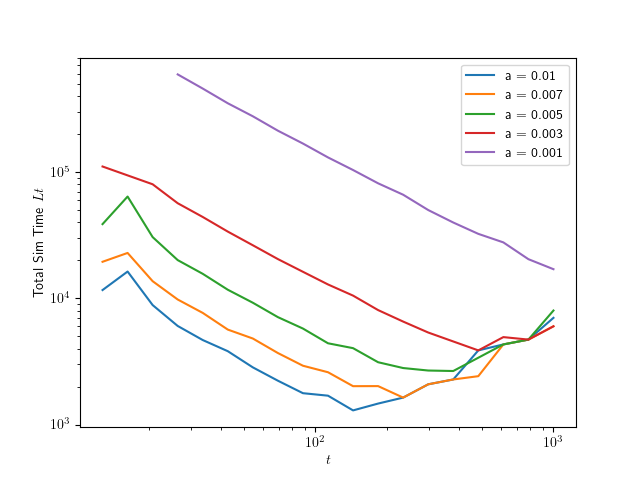
\includegraphics[width=0.75\linewidth]{numerics/data/total_time_vs_time.png}
    \caption{Total simulation time for a single qubit system to reach within trace distance of $0.05$ of the thermal state for $\beta = 4$ as a function of per-interaction simulation time $t$ . Since the total probability mass being moved at a single step is proportional to $(\alpha t)^2$, we see that increasing $\alpha$ and $t$ tend to decrease the overall cost.}\label{fig:tot_time_vs_single_time}
\end{figure}

Theorem \ref{thm:harmonic_oscillator} is helpful for giving an idea of the runtime for very low temperature states, but we cannot extend it to finite $\beta$ due to the special structure of the transition matrix in the $\beta \to \infty$ limit. For generic $\beta$ the structure of the transition matrix is tridiagonal, but it is not quite Toeplitz as the main diagonals deviate in the upper left and bottom right corners. We could try to pull these deviations into a separate matrix and treat them as perturbations to a fully Toeplitz matrix, which we can compute the spectrum of. The issue with this approach is that these deviations are on the order of $\widetilde{\alpha}^2 q(0)$ and $\widetilde{\alpha}^2 q(1)$, which are comparable to the eigenvalues of the resulting Toeplitz matrix. This means the resulting ``perturbation" is actually on the same scale as the unperturbed matrix and perturbation theory breaks down. Analytically computing the spectral gap for $\dim = 3$ reveals a hyperbolic cosecant structure, but these calculations do not scale easily to higher dimension. It seems that we are restricted to probing the runtime for higher dimensions and finite $\beta$ numerically.

Before we look at the $\beta$ dependence of the runtime our first goal will be to verify our analytic derivations and determine how close our Markov chain approximation is to the real dynamics of the channel. To do this we will track the distance to the target thermal state $\norm{\rho(\beta) - \Phi^{\circ L}(\rho(0))}_1$ as a function of $L$ as well as the theoretically computed Markov chain $\norm{\vec{p}_{\beta} - (\identity + T)^L \vec{p}_0}_1 $. This is done in Figure \ref{fig:sho_error_vs_interactions} where we plot the distance to the thermal state as a function of the number of interactions. As our remainder error is controlled by $\alpha t$ and our off-resonance error by $\alpha / \Delta_{\min}$ we include one plot that varies $\alpha$ and keeps $t$ constant and vice versa for the other plot. We find that increasing $\alpha$ for a fixed $t$ will increase the convergence rate at the cost of a higher variance in the error as well as a further deviation from the Markov chain fixed point. For fixed $\alpha$ we observe a similar behavior, as $t$ increases the convergence time reduces but the deviation from the Markov chain dynamics increases.

\begin{figure}
    \centering
    \begin{subfigure}{0.49\textwidth}
        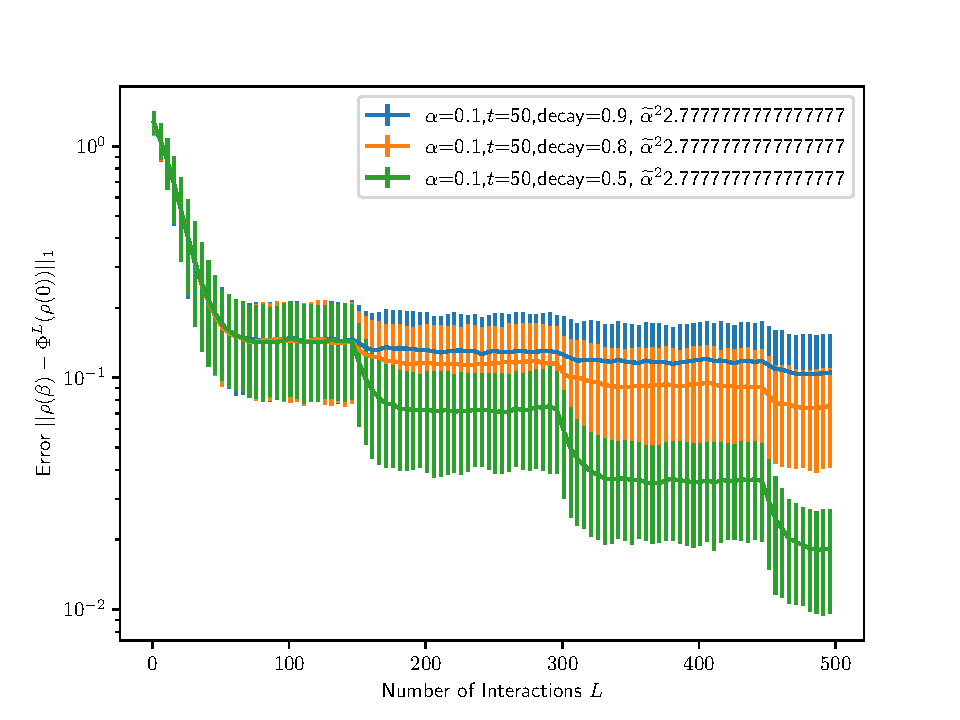
\includegraphics[width=\textwidth]{numerics/data/error_vs_interaction_fixed_time_2.pdf}     
        \caption{Varying $\alpha$ for a fixed $t$.}
    \end{subfigure}
    \begin{subfigure}{0.49\textwidth}
        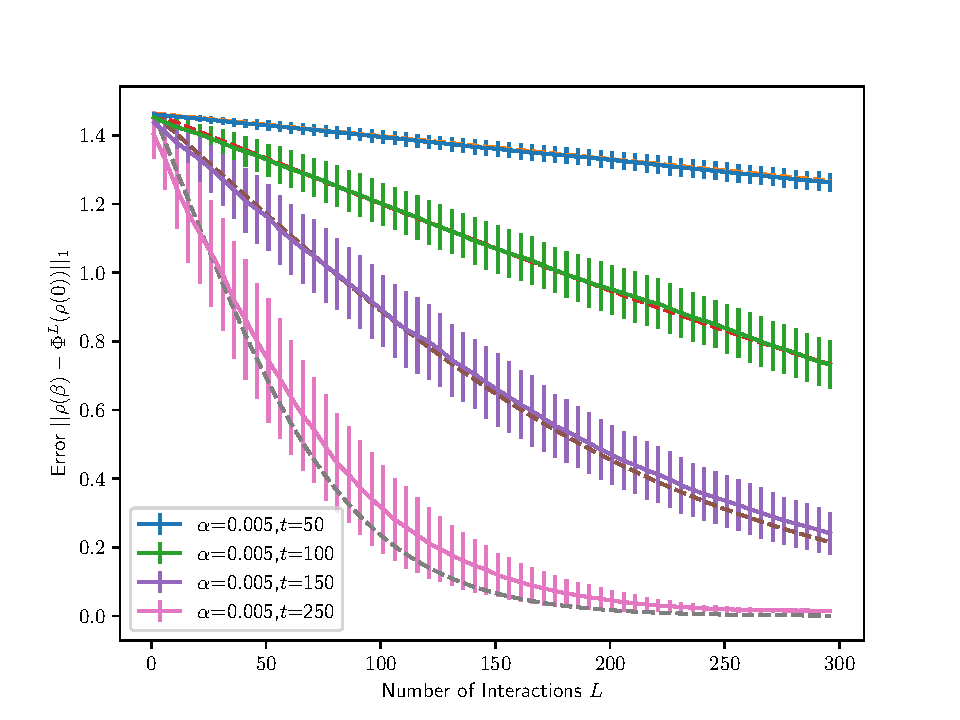
\includegraphics[width=\textwidth]{numerics/data/error_vs_interaction_fixed_time.pdf}    
        \caption{Varying $t$ for a fixed $\alpha$.}
    \end{subfigure}

    \caption{Distance from the thermal state $ \norm{\rho_S(\beta) - \Phi^{\circ L}(\rho_S(0))}_1$ as a function of the number of interactions $L$. The system is a $\dim_S = 4$ truncated harmonic oscillator and $\beta = 8$, so the prepared state has very high overlap with the ground state. We investigate the effects of $\alpha$ and $t$ on the error separately, the top plot keeps $t$ fixed and the bottom keeps $\alpha$ fixed. In both we see that increasing $\alpha$ or $t$ leads to faster convergences. The downside to the faster convergence is a larger deviation from the Markov chain behavior, which is shown in dashed lines for each parameter setting. This could be an issue for very accurate state preparations as $\epsilon \to 0$.}
    \label{fig:sho_error_vs_interactions}
\end{figure}

\begin{figure}[t]
    \centering
    \begin{subfigure}{0.45\textwidth}
    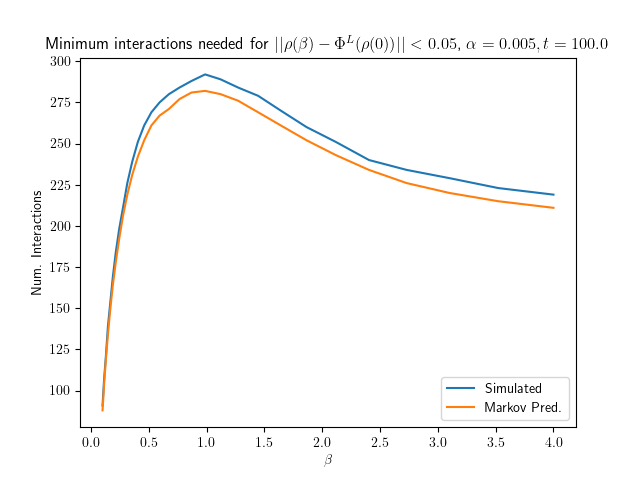
\includegraphics[width=\textwidth]{numerics/data/sho_l_vs_beta.png}
    \caption{Minimum Interactions vs. $\beta$, $\dim = 4$}
    \label{fig:sho_l_vs_beta_dim_4}
    \end{subfigure}
    \begin{subfigure}{0.45\textwidth}
    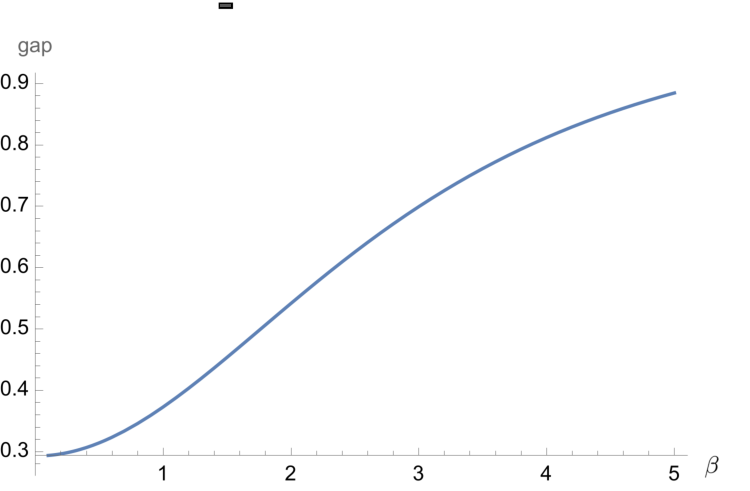
\includegraphics[width=\textwidth]{numerics/data/spec_gap_dim_4.pdf}
    \caption{Spectral Gap $\lambda_\star(\beta)$ vs. $\beta$, $\dim = 4$}
    \label{fig:sho_spectral_gap_vs_beta}
    \end{subfigure}
    \hfill
    \begin{subfigure}{0.5\textwidth}
    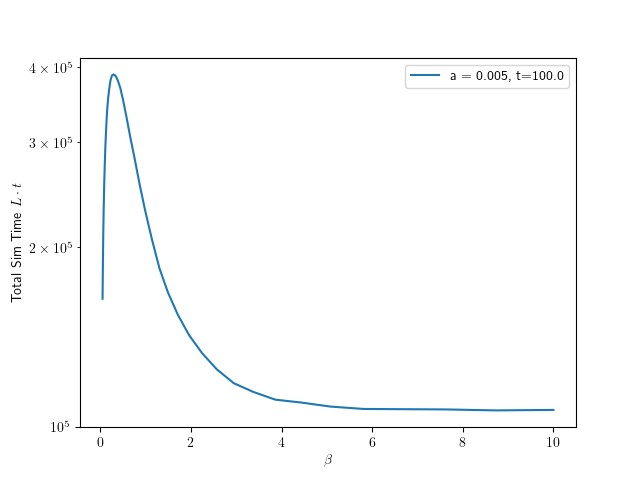
\includegraphics[width=\textwidth]{numerics/data/sho_big_peak.png}
    \caption{Minimum Interactions vs. $\beta$, $\dim = 10$}
    \label{fig:sho_l_vs_beta_dim_10}
    \end{subfigure}
    \caption{Demonstration of $\beta$ dependence of the thermalizing channel $\Phi$ for the truncated harmonic oscillator.}
    \label{fig:sho_total_time_vs_beta}
\end{figure}


Now that we have numerically verified the validity of our channel as a thermalizing channel as well as the $\alpha$ and $t$ behavior of our Markov chain, we turn our attention to the total simulation time as a function of $\beta$. This is important as our runtime results for the single qubit are independent of $\beta$ and the only runtime results we have for the harmonic oscillator is for the ground state $\beta \to \infty$. Our numeric results are contained in Figure \ref{fig:sho_total_time_vs_beta}. The method we used is to start our simulation at $\rho = \frac{\identity}{\dim_S}$, as we need a state that commutes with $H_S$ and is easy to prepare. We then find the smallest number of interactions needed for our state to have an average trace distance of less than 0.05, averaged over 100 samples, using values of $\alpha$ and $t$ found by trial and error. We find that even for systems as small as $\dim_S = 4$ there is a nontrivial dependence of the runtime on $\beta$. The total simulation time increases with $\beta$, as one would initially expect, until it reaches a peak and then decreases, indicating colder temperatures can converge \emph{quicker} than warmer temperatures when starting from an infinite temperature initial state. This bump becomes noticeably more pronounced as the dimension increases, see Figure \ref{fig:sho_total_time_vs_beta}. Our explanation for this phenomena is a temperature dependence of the Markov chain spectral gap that is different than the temperature dependence of the distance between the starting state and the thermal state. 


We first demonstrate the thermalization runtime for the truncated harmonic oscillator, however this time we characterize the runtime needed to thermalize as a function of our knowledge of the spectrum. To parametrize this, as we simulate our repeated interactions channel we sample the environment gaps $\gamma$ from a mixture distribution of Gaussians centered around each eigenvalue difference with a width of $\sigma$. As we vary $\sigma$ from 0 to the maximum eigenvalue difference in the Hamiltonian, we are effectively interpolating our $\gamma$ sampler from perfectly sampling the eigenvalue differences to sampling complete noise. The results in Figure \ref{fig:sho_with_noise} are promising, although we see that having no noise added to the system results in a roughly 10x lower runtime than the completely noisy $\gamma$ samples, the runtime does have a fairly stable plateau. This indicates that the algorithm should work fairly consistently without any knowledge whatsoever of the eigenvalue gaps $\Delta$.

% \begin{figure}
%     \centering
%     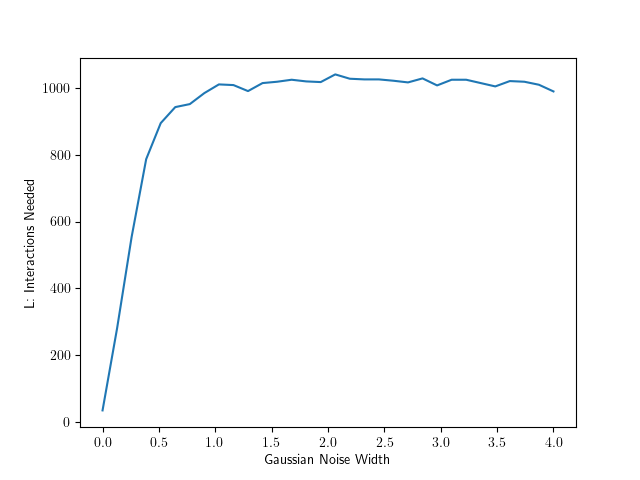
\includegraphics[width=0.5\linewidth]{numerics/data/sho_with_noise_1.png}
%     \caption{Number of interactions needed to reach a trace distance of $0.1$ away from the thermal state with $\beta = 1.0$, for a dimension 5 truncated harmonic oscillator, by sampling from the exact spectrum of the hamiltonian with the amount of added noise indicated by the x-axis. The rightmost limit of the plot is equal to the ``spectral diameter", or the largest eigenvalue minus the smallest. We can see a fairly rapid growth with added noise followed by a fairly stable plateau, indicating that even with minimal to zero knowledge of the spectrum reliable approximation to the thermal state can be prepared. }
%     \label{fig:sho_with_noise}
% \end{figure}

\section{General Systems} \label{sec:general_systems}
 Now that we have studied a single qubit and the harmonic oscillator in as much detail as possible, in this section we explore the behavior of our algorithm for more generic systems. As our algorithm ultimately boils down to a Markov chain over the eigenstates of the Hamiltonian we are unable to make any runtime claims, as that would require bounding the spectral gap of a Markov chain that depends on knowledge of the Hamiltonian eigenvalues. What we do show in this section is three-fold: we first demonstrate that if the environment temperature approaches 0 ($\beta \to \infty$), then the ground state of the system is \emph{a} fixed point, second that if the eigenvalue differences $\set{\lambda(i) - \lambda(j)}_{i, j}$ can be sampled from exactly then choosing $\Delta$ to correspond to these gaps leads the algorithm to yield the thermal state as its unique fixed point. Lastly, we demonstrate numerically that knowledge of eigenvalue gaps is not entirely necessary by preparing low temperature thermal states for Hydrogen chains without any a priori knowledge.


\subsection{Zero Knowledge - DEFCON 4} \label{sec:zero_knowledge}
We now move on to show how our algorithm performs if one has no knowledge about the eigenvalue differences $\Delta_S(i,j)$ apart from a bound on the maximum value of these differences. This is represented by choosing $\gamma$ uniformly from the interval $[0, 4 \norm{H_S}]$, which technically constitutes an upper bound on the largest $\Delta_S(i,j)$, but estimates of $\norm{H_S}$ are often readily attainable from the specification of the Hamiltonian using the triangle inequality.  We also assume that an input state that commutes with the Hamiltonian can be provided.  This is not a substantial restriction because recall that such a state can be attained from either phase estimation or from using a maximally mixed state as an input.

\begin{theorem}[Zero Knowledge Thermal State Prep] \label{thm:zero_knowledge}
    Let $H_S$ be a Hermitian matrix with no degenerate eigenvalues, $\rho$ any input state that commutes with $H_S$, and $\gamma$ a random variable chosen uniformly in the interval $[0, 4 \norm{H_S}]$a and
    let $\rho_{\rm fix}$ denote the unique fixed point of the transition dynamics $\identity + \EE_\gamma \TT_{\on}^{(\gamma)}$. The following statements then hold.
    \begin{enumerate}
\item For finite $\beta$ the thermal state is an approximate fixed point of the thermalizing channel $\EE_\gamma \Phi_\gamma$ with a deviation of
    \begin{equation}
        \norm{\rho_S(\beta) - \EE_\gamma \Phi_\gamma(\rho_S(\beta))}_1 \le \alpha^2 t e^{\beta \delta_{\min}} \norm{H_S}^{-1} \pi + 8 \frac{\alpha^2}{\delta_{\min}} + 16 \sqrt{\frac{\pi}{2}} \dim_S (\alpha t)^3.
    \end{equation}
    \item   The parameter settings
    \begin{align}
        \alpha = \frac{\delta_{\min}^4 \epsilon^{3} \lambda_\star(\beta)^{3}}{\dim_S^7 \norm{H_S}^3}, ~t = \frac{\dim_S^2 \norm{H_S}}{\epsilon \lambda_\star(\beta) \delta_{\min}^2}, \text{ and } L \in \bigotilde{\frac{\dim_S^{14} \norm{H_S}^6}{\epsilon^5 \delta_{\min}^6 \lambda_\star(\beta)^{6} }}
    \end{align}
    are sufficient to guarantee $\norm{\rho_{\rm fix} - \left(\EE_\gamma \Phi_\gamma \right)^{\circ L}(\rho)}_1 \in \bigotilde{\epsilon}$.
    The total experimental time needed is therefore
    \begin{equation}
        L \cdot t \in \bigotilde{\frac{\dim_S^{16} \norm{H_S}^7}{\delta_{\min}^8 \epsilon^6 \lambda_\star(\beta)^7}}.
    \end{equation}
   \item    The fixed point is the ground state In the $\beta \to \infty$ limit and the spectral gap is lower bounded by a constant, giving the two limits
    \begin{equation}
        \lim_{\beta \to \infty} \rho_{\rm fix} = \ketbra{1}{1} \text{ and } \lim_{\beta \to \infty} \lambda_\star(\beta) \ge 2.43.
        \end{equation}
    Substituting this bound on $\lambda_\star(\beta)$ into the choices for $\alpha, t$ and $L$ given for finite $\beta$ is sufficient to guarantee thermalization of $\left(\EE_\gamma \Phi_\gamma \right)^{\circ L}$.
    \end{enumerate}
\end{theorem}
\begin{proof}
    This proof structure will be structurally similar to the proof of Theorem \ref{thm:perfect_knowledge}. We start by understanding the fixed points of $\identity + \EE_\gamma \TT_{\on}^{(\gamma)}$, conditions for the thermal state being fixed are given in Lemma \ref{lem:fixed_point}. As the condition boils down to a detailed balance like condition, we need to compute the off-diagonal transition elements first. Starting with $i > j$ we have
    \begin{align}
        &\EE_\gamma \bra{j} \TT_{\on}^{(\gamma)}(\ketbra{i}{i})\ket{j} \nonumber \\
        &=  \widetilde{\alpha}^2 \EE_{\gamma} \frac{1}{1 + e^{-\beta \gamma}} \mathbf{I}[|\Delta_S(i,j) - \gamma| \le \delta_{\min}]  \sinc^2\left(\frac{(\Delta_S(i,j) - \gamma)t}{2}\right) \\ \nonumber \\
        &~+ \widetilde{\alpha}^2 \EE_{\gamma} \frac{e^{-\beta \gamma}}{1 + e^{-\beta \gamma}} \mathbf{I}[|\Delta_S(i,j) + \gamma| \le \delta_{\min}]  \sinc^2\left(\frac{(\Delta_S(i,j) + \gamma)t}{2}\right) \\
        &= \widetilde{\alpha}^2 \EE_{\gamma} \frac{1}{1 + e^{-\beta \gamma}} \mathbf{I}[|\Delta_S(i,j) - \gamma| \le \delta_{\min}]  \sinc^2\left(\frac{(\Delta_S(i,j) - \gamma)t}{2}\right) \\
        &= \widetilde{\alpha}^2 \frac{1}{4 \norm{H_S}} \int_{0}^{4 \norm{H_S}} \frac{1}{1 + e^{-\beta \gamma}} \mathbf{I}[|\Delta_S(i,j) - \gamma| \le \delta_{\min}]  \sinc^2\left(\frac{(\Delta_S(i,j) - \gamma)t}{2}\right) d\gamma \\
        &=  \frac{\widetilde{\alpha}^2}{4 \norm{H_S}} \int_{\Delta_S(i,j) - \delta_{\min}}^{\Delta_S(i,j) + \delta_{\min}} \frac{1}{1 + e^{-\beta \gamma}}  \sinc^2\left(\frac{(\Delta_S(i,j) - \gamma)t}{2}\right) d\gamma \\
        &= \frac{\widetilde{\alpha}^2}{2 t \norm{H_S}} \int_{-\delta_{\min} t /2}^{\delta_{\min} t / 2} \frac{1}{1 + e^{-\beta (\Delta_S(i, j) - 2 u /t)}} \sinc^2(u) du. \label{eq:zero_knowledge_transition_1}
    \end{align}
    The exact same calculation holds for $i < j$ but with a slightly different integrand
    \begin{align}
        \EE_\gamma \bra{j} \TT_{\on}^{(\gamma)}(\ketbra{i}{i})\ket{j} &= \frac{\widetilde{\alpha}^2}{2 t \norm{H_S}} \int_{-\delta_{\min} t /2}^{\delta_{\min} t / 2} \frac{e^{-\beta (\Delta_S(j,i) - 2 u /t)}}{1 + e^{-\beta (\Delta_S(j,i) - 2 u /t)}} \sinc^2(u) du,\label{eq:zero_knowledge_transition_2}
    \end{align}
    as we pick up a factor of $q(1)$ as opposed to $q(0)$. Note that we have also shown that $\EE_\gamma T_\gamma$ is ergodic, as there is a nonzero probability for any state $\ketbra{i}{i}$ to transition to any other state $\ketbra{j}{j}$ in one iteration.

    For finite $\beta$ the condition for $\rho_S(\beta)$ being a fixed point is given in Eq. \eqref{eq:detailed_balance}, repeated here as
    \begin{equation}
        \sum_{i \neq j} \frac{e^{-\beta \lambda_S(i)}}{\partfun_S(\beta)} e_j^T \EE_\gamma T_\gamma e_i - \frac{e^{-\beta \lambda_S(j)}}{\partfun_S(\beta)}  e_i^T \EE_\gamma T_\gamma e_j = 0,
    \end{equation}
    for all $j$. We can plug in our calculation for the transition coefficients for summands with $i > j$ first
    \begin{align}
        &\frac{e^{-\beta \lambda_S(i)}}{\partfun_S(\beta)} e_j^T \EE_\gamma T_\gamma e_i - \frac{e^{-\beta \lambda_S(j)}}{\partfun_S(\beta)}  e_i^T \EE_\gamma T_\gamma e_j \nonumber \\ 
        &= \frac{e^{-\beta \lambda_S(j)}}{\partfun_S(\beta)} \left( e^{-\beta \Delta_S(i,j)} \EE_\gamma \bra{j} \TT_{\on}^{(\gamma)}(\ketbra{i}{i})\ket{j} - \bra{i} \TT_{\on}^{(\gamma)}(\ketbra{j}{j})\ket{i} \right) \\
        &= \frac{e^{-\beta \lambda_S(j)}}{\partfun_S(\beta)} \frac{\widetilde{\alpha}^2}{2 t \norm{H_S}} e^{-\beta \Delta_S(i,j)} \int_{-\delta_{\min} t /2 }^{\delta_{\min} t/ 2} \frac{1 - e^{\beta 2 u / t}}{1 + e^{-\beta(\Delta_S(i,j) - 2u/t)}} \sinc^2(u) du \\
        &= \frac{e^{-\beta \lambda_S(i)}}{\partfun_S(\beta)} \frac{\widetilde{\alpha}^2}{2 t \norm{H_S}} \int_{-\delta_{\min} t /2 }^{\delta_{\min} t/ 2} \frac{1 - e^{\beta 2 u / t}}{1 + e^{-\beta(\Delta_S(i,j) - 2u/t)}} \sinc^2(u) du. \label{eq:zero_knowledge_tmp_1}
    \end{align}
    For $i < j$ we have the very similar
    \begin{align}
        &\frac{e^{-\beta \lambda_S(i)}}{\partfun_S(\beta)} e_j^T \EE_\gamma T_\gamma e_i - \frac{e^{-\beta \lambda_S(j)}}{\partfun_S(\beta)}  e_i^T \EE_\gamma T_\gamma e_j \nonumber \\ 
        &= \frac{e^{-\beta \lambda_S(j)}}{\partfun_S(\beta)} \frac{\widetilde{\alpha}^2}{2 t \norm{H_S}} \int_{-\delta_{\min} t /2 }^{\delta_{\min} t/ 2} \frac{ e^{\beta 2 u / t} - 1}{1 + e^{-\beta(\Delta_S(j, i) - 2u/t)}} \sinc^2(u) du. \label{eq:zero_knowledge_tmp_2}
    \end{align}
    Unfortunately these integrals are not 0, which can be verified numerically, and it is incredibly unclear how to make the summation over $i \neq j$ equal to 0. 
    
    Our work around this is that instead of showing that the thermal state is exactly the fixed point we can use these results to show that it is an approximate fixed point. There are a few ways we could proceed. The first way could be to compute a Taylor series for the integrand and isolate the limits in which the remainder goes to 0. Unfortunately due to the $\sinc^2(u) = \sin(u)^2 / u^2$ term this means that the overall scaling will go like $1/t$, making the total expression independent of $t$. Instead the route we will take will be to upper bound the norm $\norm{\vec{p}_{\beta} - \EE_\gamma (I + T_\gamma)\vec{p}_\beta}_1 = \norm{\EE_\gamma T_\gamma \vec{p}_\beta}$, as this norm is only 0 if $\vec{p}_\beta$ is a fixed point. We reduce this to computations we have already performed as
    \begin{align}
        \norm{\EE_\gamma T_\gamma \vec{p}_\beta}_1 &= \sum_j \abs{e_j^T \EE_\gamma T_\gamma \vec{p}_\beta } \\
        &= \sum_j \abs{\sum_{i} \frac{e^{-\beta \lambda_S(i)}}{\partfun_S(\beta)} e_j^T \EE_\gamma T_\gamma e_i } \\
        &= \sum_j \abs{\sum_{i \neq j} \frac{e^{-\beta \lambda_S(i)}}{\partfun_S(\beta)} e_j^T \EE_\gamma T_\gamma e_i - \frac{e^{-\beta \lambda_S(j)}}{\partfun_S(\beta)} e_i^T \EE_\gamma T_\gamma e_j}.
    \end{align}
    This is essentially the derivation for the fixed point conditions described in Lemma \ref{lem:fixed_point}. We now plug in Eqs. \eqref{eq:zero_knowledge_tmp_1} and \eqref{eq:zero_knowledge_tmp_2} into the above and upper bound the integral with the most obvious bounds available to get
    \begin{align}
        &\sum_j \abs{\sum_{i \neq j} \frac{e^{-\beta \lambda_S(i)}}{\partfun_S(\beta)} e_j^T \EE_\gamma T_\gamma e_i - \frac{e^{-\beta \lambda_S(j)}}{\partfun_S(\beta)} e_i^T \EE_\gamma T_\gamma e_j} \nonumber \\
        &\le \sum_j \abs{\sum_{i < j} \frac{e^{-\beta \lambda_S(i)}}{\partfun_S(\beta)} e_j^T \EE_\gamma T_\gamma e_i - \frac{e^{-\beta \lambda_S(j)}}{\partfun_S(\beta)} e_i^T \EE_\gamma T_\gamma e_j} + \sum_j  \abs{\sum_{i > j} \frac{e^{-\beta \lambda_S(i)}}{\partfun_S(\beta)} e_j^T \EE_\gamma T_\gamma e_i - \frac{e^{-\beta \lambda_S(j)}}{\partfun_S(\beta)} e_i^T \EE_\gamma T_\gamma e_j} \\
        &= \frac{\widetilde{\alpha}^2}{2 t \norm{H_S}} \sum_j \abs{\sum_{i < j} \frac{e^{-\beta \lambda_S(j)}}{\partfun_S(\beta)} \int_{-\delta_{\min} t /2 }^{\delta_{\min} t/ 2} \frac{ e^{\beta 2 u / t} - 1}{1 + e^{-\beta(\Delta_S(j, i) - 2u/t)}} \sinc^2(u) du} \nonumber \\
        &+ \frac{\widetilde{\alpha}^2}{2 t \norm{H_S}} \sum_j  \abs{\sum_{i > j} \frac{e^{-\beta \lambda_S(i)}}{\partfun_S(\beta)} \int_{-\delta_{\min} t /2 }^{\delta_{\min} t/ 2} \frac{1 - e^{\beta 2 u / t}}{1 + e^{-\beta(\Delta_S(i,j) - 2u/t)}} \sinc^2(u) du} \\
        &\le \frac{\widetilde{\alpha}^2}{2 t \norm{H_S}} \sum_j \sum_{i < j} \frac{e^{-\beta \lambda_S(j)}}{\partfun_S(\beta)} \int_{-\delta_{\min} t /2 }^{\delta_{\min} t/ 2}\abs{ \frac{ e^{\beta 2 u / t} - 1}{1 + e^{-\beta(\Delta_S(j, i) - 2u/t)}}} \sinc^2(u) du \nonumber \\
        &+ \frac{\widetilde{\alpha}^2}{2 t \norm{H_S}} \sum_j  \sum_{i > j} \frac{e^{-\beta \lambda_S(i)}}{\partfun_S(\beta)} \int_{-\delta_{\min} t /2 }^{\delta_{\min} t/ 2} \abs{ \frac{1 - e^{\beta 2 u / t}}{1 + e^{-\beta(\Delta_S(i,j) - 2u/t)}} } \sinc^2(u) du \\
        &\le \frac{\widetilde{\alpha}^2}{2 t \norm{H_S}} e^{\beta \delta_{\min}} \int_{-\delta_{\min}t/2}^{\delta_{\min}t /2} \sinc^2(u) du \left(\sum_j \frac{e^{-\beta \lambda_S(j)}}{\partfun_S(\beta)} \sum_{i < j} 1 + \sum_j \sum_{i > j} \frac{e^{-\beta \lambda_S(i)}}{\partfun_S(\beta)}  \right) \\
        &\le \frac{\widetilde{\alpha}^2 \dim_S}{t \norm{H_S}} e^{\beta \delta_{\min}} \pi \\
        &\le \alpha^2 t e^{\beta \delta_{\min}} \norm{H_S}^{-1} \pi.
    \end{align}
    For this we can have $\alpha t$, which represents the total simulation time for the random interaction $G$ be constant and still take $\alpha \to 0$ to achieve arbitrarily small error.

    Now we turn to bounding the runtime. We will let $\rho_{\rm fix}$ denote the fixed point of the dynamics. As before we break the error into two pieces
    \begin{equation}
        \norm{\rho_{\rm fix} - \left(\EE_\gamma \Phi_\gamma \right)^{\circ L}}_1 \le \norm{\rho_{\rm fix} - \left(\EE_\gamma \identity + \TT_{\on}^{(\gamma)}\right)^{\circ L} (\rho)}_1 + L(\norm{\TT_{\off}}_1 + \norm{R_{\Phi}}_1).
    \end{equation}
    Let $\lambda_\star(\beta)$ denote the spectral gap for the rescaled transition matrix $\EE_\gamma T_\gamma \cdot \left(\frac{2 \norm{H_S} (\dim + 1)}{\alpha^2 t}\right)$, as this is the dimensionful prefactor in front of the transitions derived in Eqs. \eqref{eq:zero_knowledge_transition_1} and \eqref{eq:zero_knowledge_transition_2}. Jerison's Markov Relaxation Theorem \ref{thm:markov_chain_bound} tells us that taking $L$ to satisfy
    \begin{equation}
        L \ge \frac{\dim_S}{\lambda_\star} J \in \bigotilde{\frac{\dim_S^2 \norm{H_S}}{\alpha^2 t \lambda_\star(\beta)}}
    \end{equation}
    is sufficient to guarantee $\norm{\rho_{\rm fix} - \left(\EE_\gamma \identity + \TT_{\on}^{(\gamma)}\right)^{\circ L} (\rho)}_1 \in \bigotilde{\epsilon}$. Now we balance the off-resonance and remainder errors
    \begin{equation}
        \norm{\TT_{\off}}_1 + \norm{R_{\Phi}}_1 \le \frac{8 \alpha^2}{\delta_{\min}^2} + 16 \sqrt{\frac{\pi}{2}} \dim_S (\alpha t)^3 = \frac{\alpha^2}{\delta_{\min}^2} \left( 8 + 16 \sqrt{\frac{\pi}{2}} \dim_S \alpha \delta_{\min}^2 t^3 \right),
    \end{equation}
    and we see setting $\alpha = \frac{1}{\dim_S \delta_{\min}^2 t^3}$ makes the parenthesis a constant.
    To bound the total off-resonance and remainder error we take the product
    \begin{equation}
        L(\norm{\TT_{\off}}_1 + \norm{R_{\Phi}}_1) \in \bigotilde{\frac{\dim_S^2 \norm{H_S}}{\alpha^2 t \lambda_\star(\beta)} \frac{\alpha^2}{\delta_{\min}^2}} = \bigotilde{\frac{\dim_S^2 \norm{H_S}}{ t \delta_{\min}^2 \lambda_\star(\beta)} }.
    \end{equation}
    Observe that setting $t = \frac{\dim_S^2 \norm{H_S}}{\epsilon \delta_{\min}^2 \lambda_\star(\beta)}$ is sufficient to make the above product $L(\norm{\TT_{\off}}_1 + \norm{R_{\Phi}}_1) \in\bigotilde{\epsilon}$. 

    We now turn to the $\beta \to \infty$ limit. For this we note that Lemma \ref{lem:fixed_point} guarantees that the ground state is a fixed point and that $\EE_\gamma T_\gamma$ is upper triangular. We will show the ground state is unique by computing the spectrum of $\EE_\gamma T_\gamma$. For this we take the $\beta \to \infty$ limit of the transitions in Eqs. \eqref{eq:zero_knowledge_transition_1} and \eqref{eq:zero_knowledge_transition_2}, which will give us the diagonal elements and then the spectrum. For $i > j$ we take the $\beta \to \infty$ limit of Eq. \eqref{eq:zero_knowledge_transition_1} to get
    \begin{align}
        \lim_{\beta \to \infty} \EE_\gamma \bra{j} \TT_{\on}^{(\gamma)}(\ketbra{i}{i})\ket{j} &= \frac{\widetilde{\alpha}^2}{2 t \norm{H_S}} \int_{-\delta_{\min}t/2}^{\delta_{\min}t/2} \sinc^2(u) du
    \end{align}
    and for $i < j$ we have
    \begin{equation}
        \lim_{\beta \to \infty} \EE_\gamma \bra{j} \TT_{\on}^{(\gamma)}(\ketbra{i}{i})\ket{j} = 0.
    \end{equation}
    We denote the $\sinc$ integration above as
    \begin{equation}
        I_{\sinc}(t) \coloneqq \int_{-\delta_{\min}t/2}^{\delta_{\min} t/2} \sinc^2(u) du,
    \end{equation}
    and we will show later that this is constant for $\dim_S \ge 3$. Now these transitions allow us to compute the diagonal elements
    \begin{align}
        \lim_{\beta \to \infty} \EE_\gamma \bra{i} \TT_{\on}^{(\gamma)}(\ketbra{i}{i}) \ket{i} &= - \sum_{j \neq i} \lim_{\beta \to \infty} \EE_\gamma \bra{j} \TT_{\on}^{(\gamma)}(\ketbra{i}{i}) \ket{j} \\
        &= - \sum_{j < i} \lim_{\beta \to \infty} \EE_\gamma \bra{j} \TT_{\on}^{(\gamma)}(\ketbra{i}{i}) \ket{j} \\
        &= - \frac{\widetilde{\alpha}^2}{2 t \norm{H_S}} (i - 1) I_{\sinc}(t).
    \end{align}
    This gives a spectrum for $\EE_\gamma T_\gamma$ as 0 and $- \frac{\widetilde{\alpha}^2}{2 t \norm{H_S}} (i - 1) I_{\sinc}(t)$ for $i > 1$. This shows the ground state is the unique fixed point as 0 has multiplicity 1 in the spectrum. Further the spectral gap of the rescaled transition matrix $\lambda_\star(\beta)$ is then given by
    \begin{equation}
        \lim_{\beta \to \infty} \lambda_\star(\beta) = I_{\sinc}(t).
    \end{equation}
    We can repeat the analysis for finding suitable values for $\alpha, t, $ and $L$ to guarantee thermalization and we find that 
    \begin{equation}
        \alpha = \frac{1}{\dim_S \delta_{\min}^2 t^3}, ~ t = \frac{4 \dim_S^2 \norm{H_S}}{\epsilon \delta_{\min}^2}, \text{ and } L \in \bigotilde{\frac{\dim_S^2 \norm{H_S}}{\alpha^2 t}}
    \end{equation}
    are sufficient to guarantee $\norm{\ketbra{1}{1} - \left( \EE_\gamma \Phi_\gamma\right)^{\circ L} (\rho)}_1 \in \bigotilde{\epsilon}$.

    Our final task is to show that our justification of $I_{\sinc}(t)$ as constant is valid. Using the choice of $t$ directly above
    \begin{align}
        I_{\sinc}(t) = \int_{-\delta_{\min} t /2}^{\delta_{\min} t /2}  \sinc^2(u) du = 2 \int_{0}^{ \frac{\dim_S^2 4 \norm{H_S}} {\epsilon \delta_{\min}}} \sinc^2(u) du. \label{eq:zero_knowledge_sinc_integral}
    \end{align}
    Now we note that this integral is monotonic with respect to the upper limit of integration with a final value of $\lim_{t \to \infty} I_{\sinc}(t) = \pi$. We note that we can capture a significant amount of this integral by just requiring the upper limit to be greater than the first zero of sinc located at $\frac{\pi}{2}$, which is true if $\epsilon \le \frac{4 \dim_S^2 \norm{H_S}}{\pi \delta_{\min}}$. This value can be computed as $2 \int_0^{\pi / 2} \sinc^2(u) du \ge 2.43$. This can be guaranteed by noting that $\epsilon$ can be at most 2, so the upper limit in Eq. \eqref{eq:zero_knowledge_sinc_integral} is satisfied if
    \begin{align}
    \epsilon \le 2 \le \frac{3^2}{\pi} \le \frac{\dim_S^2}{\pi} \le \frac{\dim_S^2 4 \norm{H_S}}{\pi \delta_{\min}},
\end{align}
as $\delta_{\min} \le 4 \norm{H_S}$. This shows that for our choice of $t$ then $|I_{\sinc}(t) - \pi| \le 0.71$, rendering it asymptotically constant.
\end{proof}

% As we have now shown that for ground state preparation our Markov transition matrix is upper triangular we can take advantage of this to compute the spectral properties of $I + T$. This is essentially the framework for the following two theorems in which we explore how much simulation time and how many interactions are sufficient, but not necessary, for our thermalizing channel to leave the system $\epsilon$ close to the ground state. In Theorem \ref{thm:ground_state} we find that  having zero knowledge of the eigenvalue differences of the system does not prevent one from preparing the ground state; this makes intuitive sense as we are able to cool even quantum systems to very low temperatures without tuning our refrigerators to the spectrum of each sample being cooled. In Theorem \ref{thm:ground_state_prep_perfect} we demonstrate how turning ignorance of the eigenvalue differences into perfect knowledge of the differences does make an asymptotically significant reduction in the total simulation time.
% \begin{theorem}[Zero Knowledge Ground State Preparation] \label{thm:ground_state}
%     Let $H_S$ be a non-degenerate Hamiltonian acting on a Hilbert space with dimension $\dim_S \ge 3$, $\rho$ any input state such that $[\rho, H_S] = 0$, $\delta_{\min}$ as defined in Eq. \eqref{eq:delta_min_def}, and $\gamma$ a random variable chosen uniformly in the interval $[0, 4 \norm{H_S}]$. In the limit as $\beta \to \infty$ the output of the expected thermalizing channel $\EE_\gamma \Phi_\gamma$ repeated $L$ times is $\epsilon$ close to the ground state
%     \begin{equation}
%         \lim_{\beta \to \infty} \norm{\rho_S(\beta) - (\EE_\gamma \Phi_\gamma)^{\circ L} (\rho)}_1 \in \widetilde{O}(\epsilon).
%     \end{equation}
%     To achieve this error it is sufficient to use the following parameters for $\Phi_{\gamma}$
%     \begin{align}
%         \alpha = \frac{\epsilon^3 \delta_{\min}}{\dim_S^7 \norm{H_S}^3 }, \quad t = \frac{\dim_S^2 \norm{H_S}}{\epsilon \delta_{\min}},
%     \end{align}
%     and at least 
%     \begin{equation}
%         L \in \widetilde{O} \left( \frac{\dim_S^2 \norm{H_S}}{\alpha^2 t}\right)
%     \end{equation}
%     applications of the expected channel.
%     Therefore, the total simulation time required to prepare the ground state is
%     \begin{equation}
%         Lt \in \widetilde{O}\left( \frac{\dim_S^{16} \norm{H_S}^7}{\epsilon^{6} \delta_{\min}^8} \right).
%     \end{equation}
% \end{theorem}
% \begin{proof}
%     This proof will proceed in a few stages: first we will break down the distance of the output of the repeated channel into a Markovian error and a remainder term error, second we then compute the expected diagonal elements which gives us the spectrum, third we use this to compute the number of interactions needed for the Markovian error to be less than $\epsilon$, and lastly we use this value of $L$ to choose $\alpha$ and $t$ that make the remainder and off-resonance error less than $\bigotilde{\epsilon}$. This then will give the final runtime.
    
%     We will denote the channel for a given value of $\gamma$ as $\Phi_{\gamma}$ and the on-resonance map $\mathcal{T}_{\gamma}^{(\on)}$. A further simplification we will make is we will assume a $\beta \to \infty$ limit throughout. We start by splitting our error into two parts, the distance to the fixed point of the Markov chain and the off-resonance and remainder errors
% \begin{align}
%     \norm{\rho_S(\infty) - \EE_\gamma \left[\Phi_{\gamma}\right]^{\circ L} (\rho)}_1 \le \norm{\rho_S(\infty) - \left(\EE_{\gamma}\left[  \identity + \mathcal{T}_\gamma^{(\on)}  \right] \right)^{\circ L}(\rho)}_1 + L \left(\norm{\mathcal{T}_{\off}}_1 + \norm{R_{\Phi}}_1\right),
% \end{align}
% where we do not include the $\gamma$ averaging for the error terms as they are independent of the choice of $\gamma$.

% Using Lemma \ref{lem:fixed_point} we know that $\EE_\gamma T_\gamma$ is upper triangular and that $e_1$ is a fixed point. As Lemma \ref{lem:fixed_point} holds for arbitrary $\gamma$ it also holds for the expected transition matrix. We now need to compute what the diagonal entries are exactly, as these directly encode the spectrum of the Markov chain. As Lemma \ref{lem:fixed_point} shows that $\EE_\gamma e_1^T T_\gamma e_1 = 0$ we can compute the $i > 1$ diagonal entries as
% \begin{align}
%     \EE_\gamma \lim_{\beta \to \infty} e_i^T T_\gamma e_i &= \EE_\gamma \lim_{\beta \to \infty} \bra{i} \TT_\gamma^{(\on)}(\ketbra{i}{i}) \ket{i} \\
%     &= - \EE_\gamma \lim_{\beta \to \infty} \sum_{j \neq i} \bra{j} \TT_\gamma^{(\on)}(\ketbra{i}{i}) \ket{j} \\
%     &= - \EE_\gamma \lim_{\beta \to \infty} \sum_{j < i} \widetilde{\alpha}^2 \frac{1}{1 + e^{-\beta \gamma}} \mathbf{I}[|\Delta_S(i,j) - \gamma| \le \delta_{\min}] \sinc^2 \left( \frac{(\Delta_S(i, j) - \gamma) t}{2} \right) \nonumber \\
%     &\quad - \EE_\gamma \lim_{\beta \to \infty} \sum_{j > i} \widetilde{\alpha}^2 \frac{e^{-\beta \gamma}}{1 + e^{-\beta \gamma}} \mathbf{I}[|\Delta_S(i, j) + \gamma| \le \delta_{\min}] \sinc^2 \left( \frac{(\Delta_S(i, j) + \gamma) t}{2} \right) \\
%     &= - \EE_\gamma  \sum_{j < i} \widetilde{\alpha}^2  \mathbf{I}[|\Delta_S(i,j) - \gamma| \le \delta_{\min}] \sinc^2 \left( \frac{(\Delta_S(i, j) - \gamma) t}{2} \right) \lim_{\beta \to \infty} \frac{1}{1 + e^{-\beta \gamma}} \nonumber \\
%     &\quad - \EE_\gamma \sum_{j > i} \widetilde{\alpha}^2 \mathbf{I}[|\Delta_S(i, j) + \gamma| \le \delta_{\min}] \sinc^2 \left( \frac{(\Delta_S(i, j) + \gamma) t}{2} \right) \lim_{\beta \to \infty} \frac{e^{-\beta \gamma}}{1 + e^{-\beta \gamma}} \\
%     &= -   \sum_{j < i} \widetilde{\alpha}^2 \EE_\gamma \mathbf{I}[|\Delta_S(i,j) - \gamma| \le \delta_{\min}] \sinc^2 \left( \frac{(\Delta_S(i, j) - \gamma) t}{2} \right). \label{eq:ground_state_tmp_1}
% \end{align}

% Now we compute the $\gamma$ expectation value. We will choose a uniform distribution for $\gamma$ from 0 to $4 \norm{H_S}$. The rationale for this is that we would like for every $\sinc$ integral in the above to evaluate to the same quantity. This means $\gamma$ needs to be uniformly distributed within $\pm \delta_{\min}$ of each value of $\Delta_S(i,j)$. The lower limit $\gamma$ must take is $\min |\Delta(i,j)| - \delta_{\min}$. As $\delta_{\min} \le \min |\Delta_S(i,j)|$ this lower limit is 0. The upper range that $\gamma$ can take will be $\max |\Delta_S(i,j)| + \delta_{\min}$, which $\max |\Delta_S(i,j)| \le 2 \norm{H_S}$, and we can upper bound $\delta_{\min} \le 2 \norm{H_S}$ as well. This gives the upper range of the required value of $\gamma$ as $4 \norm{H_S}$. As we are assuming no knowledge of the eigenvalue differences we then sample $\gamma$ uniformly within $[0, 4 \norm{H_S}]$.


% Using this distribution of $\gamma$ allows us to compute the expectation values as
% \begin{align}
%     &\EE_\gamma \mathbf{I}[|\Delta_S(i,j) - \gamma| \le \delta_{\min}] \sinc^2 \left( \frac{(\Delta_S(i, j) - \gamma) t}{2} \right) \nonumber \\
%     &= \int_0^{4 \norm{H_S}} \mathbf{I}[|\Delta_S(i,j) - \gamma| \le \delta_{\min}] \sinc^2 \left( \frac{(\Delta_S(i, j) - \gamma) t}{2} \right) \frac{1}{4 \norm{H_S}} d\gamma \\
%     &= \frac{1}{4 \norm{H_S}} \int_{\Delta_S(i,j) - \delta_{\min}}^{\Delta_S(i,j) + \delta_{\min}} \sinc^2 \left( \frac{(\Delta_S(i, j) - \gamma) t}{2} \right) d\gamma \\
%     &= \frac{1}{4 \norm{H_S}} \int_{-\delta_{\min}}^{\delta_{\min}} \sinc^2 \left( \frac{\widetilde{\gamma} t}{2} \right) d\widetilde{\gamma} \\
%     &= \frac{1}{2 \norm{H_S} t} \int_{-\delta_{\min} t/2}^{\delta_{\min} t/2} \sinc^2 (u) du ,\label{eq:ground_state_expect_gamma_1}
% \end{align}
% where we label the last integral with
% \begin{equation}
%     I_{\sinc}(t) \coloneqq  \int_{-\delta_{\min} t/2}^{\delta_{\min} t/2} \sinc^2 (u) du  . \label{eq:ground_state_prep_sinc_integral}
% \end{equation}
% For now we claim that $I_{\sinc}(t) \in \widetilde{\Theta}(1)$ without proof and will therefore drop it from asymptotic expressions. We show that this is valid at the end of the proof.

% Plugging Eq. \eqref{eq:ground_state_expect_gamma_1} into Eq. \eqref{eq:ground_state_tmp_1} we arrive at the final expression for the expected diagonal elements
% \begin{align}
%     \EE_\gamma \lim_{\beta \to \infty} e_i^T T_\gamma e_i &= -   \sum_{j < i}  \frac{\widetilde{\alpha}^2}{2 \norm{H_S} t} I_{\sinc}(t) = - \frac{\widetilde{\alpha}^2 (i - 1)}{2 \norm{H_S} t} I_{\sinc}(t)
% \end{align}
% For the remainder of the proof we will not write the $\beta \to \infty$ limit and take it as implicit. Now we can compute the characteristic polynomial $p_T(x) = \det(x I - \EE_\gamma T_\gamma)$, the roots of which are the eigenvalues of $\EE_\gamma T_\gamma$. Since the determinant of an upper triangular matrix is the product of the diagonals we have
% \begin{align}
%     p_T(x) &= \det(x I - \EE_\gamma T_\gamma) \\
%     &= e_1^T(x I - \EE_\gamma T_\gamma)e_1 \prod_{i = 2}^{\dim_S} e_i^T (x I - \EE_\gamma T_\gamma) e_i \\
%     &= x \prod_{i = 2}^{\dim_S} \left( x + \frac{\widetilde{\alpha}^2 (i - 1)}{2 \norm{H_S} t} I_{\sinc}(t)\right). \label{eq:ground_state_characteristic_poly}
% \end{align}
% As this polynomial is already factored the roots are $x = 0$ and $x = - \frac{\widetilde{\alpha}^2 (i - 1)}{2 \norm{H_S} t} I_{\sinc}(t)$, giving a gap of 
% \begin{equation}
%     \lambda_\star = \frac{\widetilde{\alpha}^2}{2 \norm{H_S} t} I_{\sinc}(t). \label{eq:ground_state_spectral_gap}
% \end{equation}
% Further, we see that 0 is an eigenvalue with multiplicity 1. This confirms that the ground state is the unique fixed point of $\EE_\gamma (\identity + \TT_\gamma^{(\on)})$.

% The spectral gap $\lambda_\star$ now allows us to compute the asymptotic runtime of our algorithm. Using Jerison's Markov mixing Theorem \ref{thm:markov_chain_bound} we see that the following value of $L$
% \begin{align}
%     L &\ge \frac{\dim_S}{\lambda_\star} \left( 2\log \frac{1}{\lambda_{\star}} + 4(1 + \log 2)+ \frac{1}{\dim_S} (2 \log \left( \frac{1}{\epsilon} \right) - 1)\right) \\
%     L &\in \widetilde{\Omega} \left( \frac{\dim_S t \norm{H_S}}{\widetilde{\alpha}^2 } \right) \\
%     &= \widetilde{\Omega} \left( \frac{\dim_S^2 \norm{H_S}}{\alpha^2 t }\right)
% \end{align}
% is sufficient to guarantee that $\norm{\ketbra{1}{1} - \left(\EE_\gamma \lim_{\beta \to \infty} \identity + \TT_\gamma^{(\on)}\right)^{\circ L}(\rho)}_1 \le \epsilon$.


% Our penultimate task is to bound the off-resonance and remainder error term, given in Theorems \ref{thm:second_order_transition} and \ref{thm:remainder_bound} as
% \begin{align}
%     \norm{\TT_{\off}}_1 + \norm{R_{\Phi}}_1 &\le \frac{8 \alpha^2}{\delta_{\min}^2} + 16 \sqrt{\frac{\pi}{2}} \dim_S (\alpha t)^3 = \frac{\alpha^2}{\delta_{\min}^2} \left(8 + 16 \sqrt{\frac{\pi}{2}} \dim_S \alpha t^3 \delta_{\min}^2 \right).
% \end{align}
% Now we choose $\alpha = \frac{1}{\dim_S t^3 \delta_{\min}^2}$ to make the contributions within the parenthesis $\widetilde{\Theta}(1)$. Our last task is to guarantee that $L(\norm{\TT_{\off}}_1  + \norm{R_{\Phi}}_1) \in \widetilde{O}(\epsilon)$.
% Reducing the asymptotic expressions to isolate the effects of $t$ we find
% \begin{align}
%     L(\norm{\TT_{\off}}_1  + \norm{R_{\Phi}}_1) &\in \widetilde{O}\parens{\frac{\dim_S t\norm{H_S} \alpha^2}{\widetilde{\alpha}^2 \delta_{\min}^2 }} = \widetilde{O}\parens{\frac{\dim_S^2 \norm{H_S}}{t \delta_{\min}^2 }}.
% \end{align}
% We can make this expression $\widetilde{O}(\epsilon)$ by setting
% \begin{equation}
%     t = \frac{\dim_S^2 8 \norm{H_S}}{\epsilon \delta_{\min}^2}.\label{eq:ground_state_prep_time}
% \end{equation}
% This then gives a final runtime of
% \begin{align}
%     Lt &\in \widetilde{O} \parens{\frac{\dim_S^2 \norm{H_S}}{\alpha^2}} = \widetilde{O} \parens{\dim_S^4 t^6 \delta_{\min}^4 \norm{H_S}} = \widetilde{O} \parens{\frac{\dim_S^{16} \norm{H_S}^7}{\epsilon^{6} \delta_{\min}^8}}.
% \end{align}

% We now verify that $I_{\sinc}(t) \in \widetilde{\Theta}(1)$ given our chosen value of $t$. By substituting Eq. \eqref{eq:ground_state_prep_time} into the definition in Eq. \eqref{eq:ground_state_prep_sinc_integral} we get
% \begin{equation}
%     I_{\sinc}(t) = \int_{-\delta_{\min} t/2}^{\delta_{\min} t/2} \sinc^2 (u) du = 2 \int_{0}^{\frac{\dim_S^2 4 \norm{H_S}}{\epsilon \delta_{\min}}} \sinc^2 (u) du .
% \end{equation}
% We first remark that because $\sinc^2 \ge 0$ this integral is monotonic with respect to the upper limit. We note that the asymptotic value of the expression is $\lim_{t \to \infty} I_{\sinc}(t) = \pi$. By requiring that the upper limit be larger than the first zero of $\sinc^2$, located at $\pi / 2$, we have $2 \int_{0}^{\pi / 2} \sinc^2(u) du \ge 2.43 $. This gives us that requiring 
% \begin{equation}
%     \epsilon \le \frac{\dim_S^2 4 \norm{H_S}}{\pi \delta_{\min}}
% \end{equation}
% guarantees that $|I_{\sinc}(t) - \pi| \le 0.72 $, which is clearly $\widetilde{\Theta}(1)$. We show that this inequality is always satisfied for $\dim_S \ge 3$, as trace distances between quantum states are always less than 2 we can write
% \begin{align}
%     \epsilon \le 2 \le \frac{3^2}{\pi} \le \frac{\dim_S^2}{\pi} \le \frac{\dim_S^2 4 \norm{H_S}}{\pi \delta_{\min}},
% \end{align}
% as $\delta_{\min} \le 4 \norm{H_S}$.
% \end{proof}
 
This poor scaling is a byproduct of a few loose bounds. First, the number of interactions needed for the Markov chain to converge, from Jerison's Theorem \ref{thm:markov_chain_bound}, is incredibly loose. This is due to the guarantee of convergence for an arbitrary input state, it is unclear if this bound could be improved if promises of overlap with the ground state on the input state are provided. Second, the lack of knowledge of the eigenvalue differences introduces an incredibly costly $1 / t$ factor into the spectral gap. This then propagates through $L$ to make the runtime significantly worse. Third, we suspect that the remainder bound could potentially be improved to $\bigo{\alpha^4}$. This could be shown by utilizing the fact that the eigenvalues of $G$ are Gaussian, meaning their third moment is 0. The computation of the $G$ eigenvalue moments is what shows the $\bigo{\alpha}$ term in the weak expansion is 0 and could show that the order correction is potentially 0 as well. This would allow for $\alpha$ to scale as $1 / t^2$ as opposed to $1 / t^3$ and could lead to significant asymptotic improvements. A further conjecture, explored in Section \ref{sec:numeric_experiments}, is that the product $\alpha t$ which represents the total time evolution of the random matrix $G$, should remain \emph{constant} with respect to $t$. This would then lead to $1/\epsilon$ scaling, which we explore numerically in Section \ref{sec:numeric_experiments}.

\subsection{Perfect Knowledge of $\Delta_S(i,j)$ - DEFCON 4} \label{sec:perfect_knowledge}

Now we move on to study a scenario when finite $\beta$ thermal states are the unique fixed point of the Markov dynamics. For this we assume sample access to the eigenvalue differences $\Delta(i,j) = \lambda(i) - \lambda(j)$, meaning if there are $\chi(i,j)$ pairs of eigenvalues with positive differences $\Delta(k,l) = \Delta(i,j) \ge 0$ then the probability we receive $\Delta(i,j)$ is $\prob{\gamma = \Delta(i,j)} = \chi(i,j) \frac{2}{\dim_S(\dim_S - 1)}$. One simplifying assumption we will make is that there are no degeneracies in the Hamiltonian and for all $i,j$ we have $\Delta(i,j) > 0$.  This assumption can be relaxed by choosing our eigenbasis such that the matrix element between any two elements within a degenerate eigenspace is zero as is typically done in degenerate perturbation theory.  Further, by taking $t$ larger than the smallest difference between eigenvalue differences we can ensure that the probability of an on-resonance transition occurring between states $i$ and $j$ is $\chi(i,j) \frac{2}{\dim_S(\dim_S - 1)}$. We can, in other words, use the definition of $\delta_{\min}$ from Eq. \eqref{eq:delta_min_def} and take $t \ge 1/ \delta_{\min}$ so that we can use Lemma \ref{lem:sinc_poly_approx} to argue that the only contribution to $\bra{j} \mathcal{T}_{\on}(\ketbra{i}{i}) \ket{j}$ is from $\gamma = \Delta(i,j)$. As $\gamma$ is a random variable this makes the transition coefficient a random variable as well. 

\begin{theorem}[Perfect Knowledge Thermal State Prep] \label{thm:perfect_knowledge}
    Let $H_S$ be a Hermitian matrix with no degenerate eigenvalues, $\rho$ any input state that commutes with $H_S$ , and let $\gamma$ be a random variable with distribution $\prob{\gamma = \Delta(i,j)} = \frac{\eta_\Delta(i,j)}{\binom{\dim_S}{2}}$. For arbitrary $\beta$ the thermal state can be prepared with controllable error
    \begin{equation}
        \norm{\rho_S(\beta) - \left(\EE_\gamma \Phi_\gamma \right)^{\circ L}(\rho)}_1 \in \bigotilde{\epsilon}
    \end{equation}
     with the following parameter settings
     \begin{align}
         \alpha &= \frac{\delta_{\min} \epsilon^{1.5} \lambda_\star(\beta)^{1.5}}{\dim_S^7}, t = \frac{\dim_S^2}{\delta_{\min} \epsilon^{0.5} \lambda_\star(\beta)^{0.5}},\text{ and } L \in \bigotilde{\frac{\dim_S^{14}}{\epsilon^2 \lambda_\star(\beta)^3}},
     \end{align}
     where $\lambda_\star(\beta)$ is the spectral gap of the rescaled transition matrix $\EE_\gamma T_\gamma  \cdot \frac{\binom{\dim_S}{2}}{\widetilde{\alpha}^2}$. 
     This gives the total simulation time required as
     \begin{equation}
         L \cdot t \in \bigotilde{\frac{\dim_S^{16}}{\delta_{\min} \epsilon^{2.5} \lambda_\star(\beta)^{3.5}}}.
     \end{equation}
     All of the above conditions hold in the ground state limit as $\beta \to \infty$ and further we can compute a lower bound on the spectral gap as
     \begin{equation}
         \lim_{\beta \to \infty} \lambda_\star(\beta) = \min_{i > 1} \sum_{j < i} \eta_\Delta(i,j) \ge 1,
     \end{equation}
     which gives fully explicit worst-case runtime bounds for ground state preparation.
\end{theorem}
\begin{proof}
To show that the thermal state is the fixed point we will need to compute transition factors of the form $\EE_\gamma \bra{j}\TT_{\on}^{(\gamma)}(\ketbra{i}{i})\ket{j}$ for use in Lemma \ref{lem:fixed_point}. Using the on-resonance definition in Eq. \eqref{eq:on_resonance} we have for $i > j$
\begin{align}
    &\EE_\gamma \bra{j} \TT_{\on}^{(\gamma)}(\ketbra{i}{i})\ket{j} \nonumber \\
    &=  \widetilde{\alpha}^2 \EE_{\gamma} \frac{1}{1 + e^{-\beta \gamma}} \mathbf{I}[|\Delta_S(i,j) - \gamma| \le \delta_{\min}]  \sinc^2\left(\frac{(\Delta_S(i,j) - \gamma)t}{2}\right) \nonumber \\
    &~+ \widetilde{\alpha}^2 \EE_{\gamma} \frac{e^{-\beta \gamma}}{1 + e^{-\beta \gamma}} \mathbf{I}[|\Delta_S(i,j) + \gamma| \le \delta_{\min}]  \sinc^2\left(\frac{(\Delta_S(i,j) + \gamma)t}{2}\right) \\
    &= \widetilde{\alpha}^2 \sum_{\Delta_S(k,l)} \prob{\gamma = \Delta_S(k,l)} \frac{\mathbf{I}[|\Delta_S(i,j) - \Delta_S(k,l)| \le \delta_{\min}]}{1 + e^{-\beta \Delta_S(k,l)}}   \sinc^2\left(\frac{(\Delta_S(i,j) - \Delta_S(k,l)t}{2}\right) \\
    &= \widetilde{\alpha}^2 \frac{\eta_\Delta(i,j)}{\binom{\dim_S}{2}} \frac{1}{1 + e^{-\beta \Delta_S(i,j)}}.
\end{align}
$i < j$ can be computed similarly as
\begin{equation}
    \EE_\gamma \bra{j} \TT_{\on}^{(\gamma)}(\ketbra{i}{i})\ket{j} = \widetilde{\alpha}^2 \frac{\eta_\Delta(i,j)}{\binom{\dim_S}{2}} \frac{e^{-\beta \Delta_S(k,l)}}{1 + e^{-\beta \Delta_S(k,l)}}.
\end{equation}
This allows us to compute the detailed-balance like condition in Eq. \eqref{eq:detailed_balance} for $i > j$
\begin{align}
    &\frac{e^{-\beta \lambda_S(i)}}{\partfun_S(\beta)} \EE_\gamma \bra{j} \TT_{\on}^{(\gamma)}(\ketbra{i}{i}) \ket{j} - \frac{e^{-\beta \lambda_S(j)}}{\partfun_S(\beta)} \bra{i} \TT_{\on}^{(\gamma)}(\ketbra{j}{j}) \ket{i} \nonumber \\
    &= \frac{e^{-\beta \lambda_S(i)}}{\partfun_S(\beta)} \widetilde{\alpha}^2 \frac{\eta_\Delta(i,j)}{\binom{dim_S}{2}} \frac{1}{1 + e^{-\beta \Delta_S(i,j)}} - \frac{e^{-\beta \lambda_S(j)}}{\partfun_S(\beta)} \widetilde{\alpha}^2 \frac{\eta_\Delta(i,j)}{\binom{dim_S}{2}} \frac{e^{-\beta \Delta_S(i,j)}}{1 + e^{-\beta \Delta_S(i,j)}} \\
    &= \frac{\widetilde{\alpha}^2}{\partfun_S(\beta)} \frac{\eta_\Delta(i,j)}{\binom{\dim_S}{2}} \left(\frac{e^{-\beta \lambda_S(i)}}{1 + e^{-\beta \Delta_S(i,j)}} - e^{-\beta \lambda_S(j)} \frac{e^{-\beta \Delta_S(i,j)}}{1 + e^{-\beta \Delta_S(i,j)} } \right) \\
    &= 0.
\end{align}
For $i < j$ the same calculation holds
\begin{align}
    &\frac{e^{-\beta \lambda_S(i)}}{\partfun_S(\beta)} \EE_\gamma \bra{j} \TT_{\on}^{(\gamma)}(\ketbra{i}{i}) \ket{j} - \frac{e^{-\beta \lambda_S(j)}}{\partfun_S(\beta)} \bra{i} \TT_{\on}^{(\gamma)}(\ketbra{j}{j}) \ket{i} \nonumber \\
    &= \frac{e^{-\beta \lambda_S(i)}}{\partfun_S(\beta)} \widetilde{\alpha}^2 \frac{\eta_\Delta(i,j)}{\binom{dim_S}{2}} \frac{e^{-\beta \Delta_S(j, i)}}{1 + e^{-\beta \Delta_S(j, i)}} - \frac{e^{-\beta \lambda_S(j)}}{\partfun_S(\beta)} \widetilde{\alpha}^2 \frac{\eta_\Delta(i,j)}{\binom{dim_S}{2}} \frac{1}{1 + e^{-\beta \Delta_S(j, i)}} \\
    &= \frac{\widetilde{\alpha}^2}{\partfun_S(\beta)} \frac{\eta_\Delta(i,j)}{\binom{\dim_S}{2}} \left(\frac{e^{-\beta \lambda_S(j)}}{1 + e^{-\beta \Delta_S(j, i)}} - \frac{e^{-\beta \lambda_S(j)}}{1 + e^{-\beta \Delta_S(j, i)} } \right) \\
    &= 0.
\end{align}
This is sufficient to show that the thermal state $\rho_S(\beta)$ is a fixed point via Lemma \ref{lem:fixed_point}. As we have also shown that the probability of transitioning from any state $\ketbra{i}{i}$ to any other state $\ketbra{j}{j}$ is nonzero this gives a nonzero expected hitting time for any pair of states. This implies the Markov chain is ergodic and that $\rho_S(\beta)$ is the \emph{unique} fixed point.

Next we bound the runtime of the algorithm. For reasons similar to the harmonic oscillator in Section \ref{sec:harmonic_oscillator} we are unable to compute the spectral gap of the Markov matrix. We start the analysis in a similar manner by using the decomposition
\begin{equation}
    \norm{\rho_S(\beta) - \left(\EE_\gamma \Phi_\gamma\right)^{\circ L}(\rho)}_1 \le \norm{\rho_S(\beta) - \left(\EE_\gamma \identity + \TT_{\on}^{(\gamma)}\right)^{\circ L}(\rho)}_1 + L(\norm{\TT_{\off}}_1 + \norm{R_{\Phi}}_1 ).
\end{equation}
We bound the Markov error via Theorem \ref{thm:markov_chain_bound}. This theorem guarantees that choosing $L$ to satisfy
\begin{align}
    L \ge \frac{\dim_S \binom{\dim_S}{2}}{\widetilde{\alpha}^2 \lambda_\star(\beta)} J \in \bigotilde{\frac{\dim_S^4}{\alpha^2 t^2 \lambda_\star(\beta)}},
\end{align}
where $\lambda_\star(\beta)$ is the spectral gap of the rescaled transition matrix $\EE_\gamma T_\gamma \cdot \frac{\binom{\dim_S}{2}}{\widetilde{\alpha}^2}$, is sufficient for $\norm{\rho_S(\beta) - \left(\EE_\gamma \identity + \TT_{\on}^{(\gamma)}\right)^{\circ L}(\rho)}_1 \in \bigotilde{\epsilon}$. We now use this to bound the total off-resonance and remainder error after balancing the two contributions asymptotically
\begin{align}
    \norm{\TT_{\off}}_1 + \norm{R_{\Phi}}_1 \le \frac{8\alpha^2}{\delta_{\min}^2} + 16 \sqrt{\frac{\pi}{2}} \dim_S (\alpha t)^3 = \frac{\alpha^2}{\delta_{\min}^2} \left( + 16 \sqrt{\frac{\pi}{2}}  \alpha \dim_S \delta_{\min}^2 t^3\right).
\end{align}
Setting $\alpha = \frac{1}{\dim_S \delta_{\min}^2 t^3}$ is sufficient to make the parenthesis a constant. Lastly to get the total error in $\bigotilde{\epsilon}$ we multiply the above by the $L$ chosen before
\begin{align}
    L (\norm{\TT_{\off}}_1 + \norm{R_{\Phi}}_1) \in \bigotilde{\frac{\dim_S^4}{\alpha^2 t^2 \lambda_\star(\beta)} \frac{\alpha^2}{\delta_{\min}^2}} = \bigotilde{\frac{\dim_S^4}{ t^2 \delta_{\min}^2 \lambda_\star(\beta)} }.
\end{align}
Choosing
\begin{equation}
    t = \frac{\dim_S^2}{\delta_{\min} \sqrt{\epsilon \lambda_\star(\beta)}} 
\end{equation}
is sufficient to guarantee $L (\norm{\TT_{\off}}_1 + \norm{R_{\Phi}}_1) \in \bigotilde{\epsilon}$ and that the total error $\norm{\rho_S(\beta) - \left( \EE_\gamma \Phi_\gamma \right)^{\circ L}(\rho)}_1 \in \bigotilde{\epsilon}$. Combining the above results for $\alpha, L$ and $t$ yields the theorem statement for finite $\beta$. 

We now show how to calculate $\lambda_\star(\beta)$ in the $\beta \to \infty$ limit. From Lemma \ref{lem:fixed_point} we know that $\EE_\gamma T_\gamma$ will be upper triangular, meaning we can compute the spectrum if we can compute the diagonals. Using our computation of the off-diagonals from before we have for $i > 1$
\begin{align}
    \lim_{\beta \to \infty} \EE_\gamma \bra{i} \TT_{\on}^{(\gamma)}(\ketbra{i}{i}) \ket{i} &= - \lim_{\beta \to \infty} \sum_{j \neq i} \bra{j} \TT_{\on}^{(\gamma)}(\ketbra{i}{i}) \ket{j} \\
    &= - \lim_{\beta \to \infty} \sum_{j < i} \widetilde{\alpha}^2 \frac{\eta_\Delta(i,j)}{\binom{\dim_S}{2}} \frac{1}{1 + e^{-\beta \Delta_S(i,j)}} - \lim_{\beta \to \infty} \sum_{j > i} \widetilde{\alpha}^2 \frac{\eta_\Delta(i,j)}{\binom{\dim_S}{2}} \frac{e^{-\beta \Delta_S(j, i)}}{1 + e^{-\beta \Delta_S(j, i)}} \\
    &= - \frac{\widetilde{\alpha}^2}{\binom{\dim_S}{2}} \sum_{j < i} \eta_\Delta(i,j).
\end{align}
For $i = 1$ as we know the ground state is fixed we have $\lim_{\beta \to \infty} \EE_\gamma \bra{1} \TT_{\on}^{(\gamma)}(\ketbra{1}{1}) \ket{1} = 0$. This gives the spectrum of $\EE_\gamma T_\gamma$ as 0 and $- \frac{\widetilde{\alpha}^2}{\binom{\dim_S}{2}} \sum_{j < i} \eta_\Delta(i,j)$ for all $i > 1$. From this spectrum we can conclude that the ground state is the \emph{unique} fixed point as 0 has multiplicity 1 in the spectrum and further that the spectral gap can be bounded from below as
\begin{align}
    \lim_{\beta \to \infty} \lambda_\star(\beta) = \min_{i > 1} \sum_{j < i} \eta_\Delta(i,j) \ge 1.
\end{align}
\end{proof}




\subsection{Numerics - DEFCON 3} \label{sec:numeric_experiments}



We now have a rigorous understanding of the correctness of our algorithm: for a single qubit system we have a complete characterization of the knowledge needed for the spectral gap $\Delta$ to prepare a thermal state, for harmonic oscillators we were able to prove that the thermal state is the unique fixed point given the oscillator gap $\Delta$ along with runtime bounds for preparing the ground state, and finally for general systems we showed that the ground state is \emph{always} a fixed point of the dynamics and if sample access to the spectral differences of the Hamiltonian is available then the thermal state is the unique fixed point. As we have seen throughout these proofs rely on computing fixed points and spectral gaps of Markov chains, a notoriously challenging problem. As a result of the difficulty of analyzing generic Markov chains analytically we are forced to rely on numerics to assess the runtime of the algorithm for various benchmark systems. It remains an open question if theoretically derived bounds on the spectral gaps of the Markov chain dynamics can be produced without knowledge of the spectral differences of the Hamiltonian. 


We now move on to more realistic benchmark systems, Hydrogen chains. These Hamiltonians are constructed via an active space computation of either 2 or 3 Hydrogen nuclei spaced equally apart with a reduced active space calculation for the electrons. The Coulomb Hamiltonian is then computed using OpenFermion~\cite{mcclean2020openfermion}. We first demonstrate that our algorithm works with very naive guesses for $\gamma$, at first we sample $\gamma$ from a Gaussian centered about the average energy level $\trace{H_S} / \dim_S$ with a standard deviation of $2 \norm{H_S}$. We plot the trace distance to the thermal state as a function of the number of interactions in Figure \ref{fig:h_chain_error}. This figure shows that the algorithm is able to achieve very accurate approximations to the thermal state for modest choices of parameters. 

\begin{figure}
    \centering
    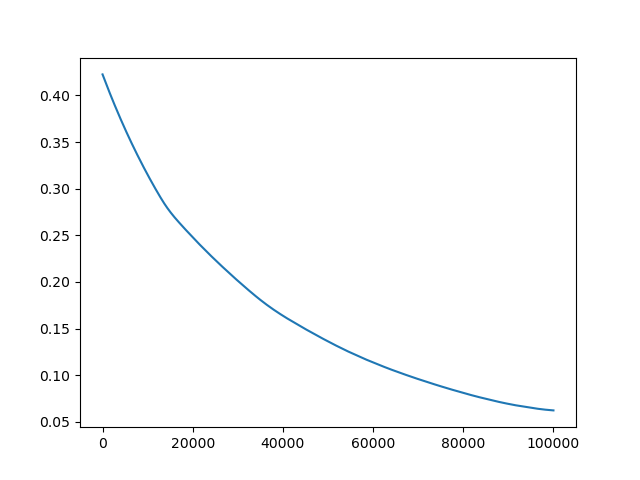
\includegraphics[width=0.45\linewidth]{numerics/data/h2_chain_2.png}
    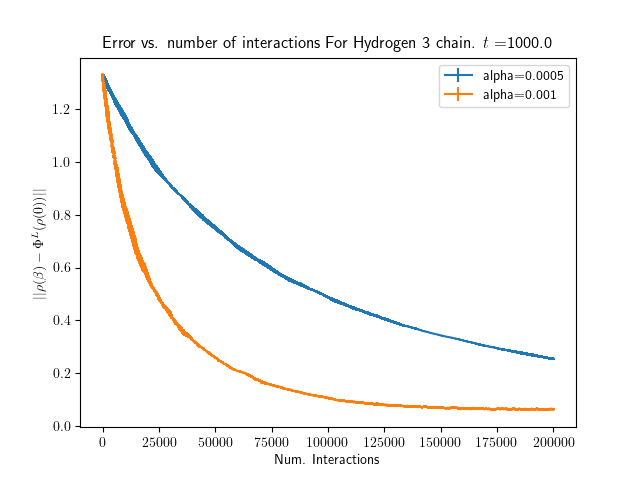
\includegraphics[width = 0.45\linewidth]{numerics/data/h3_chain_7.png}
    \caption{Hydrogen-2 and Hydrogen-3 chain distance to thermal state vs number of interactions. YES THIS IS A BAD PLOT IT NEEDS TO BE RERAN WITH LABELS.}
    \label{fig:h_chain_error}
\end{figure}

To provide further evidence that our algorithm should be able to work with bad or noisy guesses for the environment gaps $\gamma$ we repeat our noise added experiment from the simple harmonic oscillator. As our Hamiltonians are still relatively small we can compute the eigenvalue spectrum exactly and use this to sample values of $\gamma$. By adding in noise to these samples until the noise added is on the same magnitude as the spectral diameter we can study how important it is to have clean samples of $\gamma$ from the eigenvalue spectrum. Our results demonstrate that not only are clean samples not necessary, but they seem to provide less of an advantage for the larger system of the Hydrogen-3 chain compared to the Hydrogen-2 chain, and much less of an advantage than for the Harmonic Oscillator. It seems so long as one can provide an upper and lower bound on the eigenvalues for $H_S$, even random sampling for $\gamma$ should be sufficient to prepare high accuracy thermal state approximations. It remains an open problem if this can be guaranteed analytically by constructing a $\gamma$-averaged Markov chain transition matrix.

\begin{figure}
    \centering
    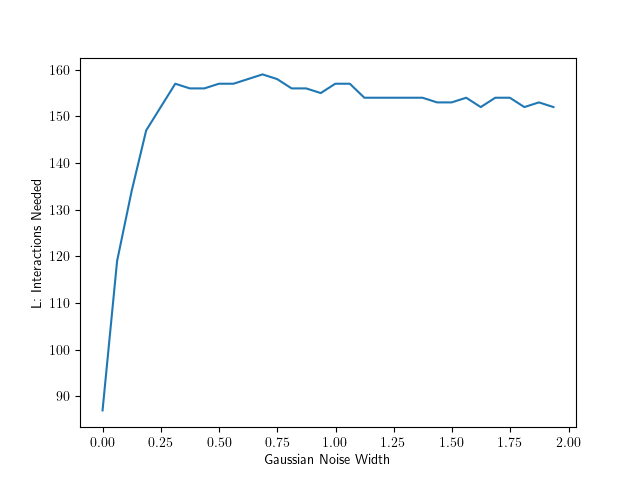
\includegraphics[width=0.475\linewidth]{numerics/data/h_chain_with_noise_1.png}
    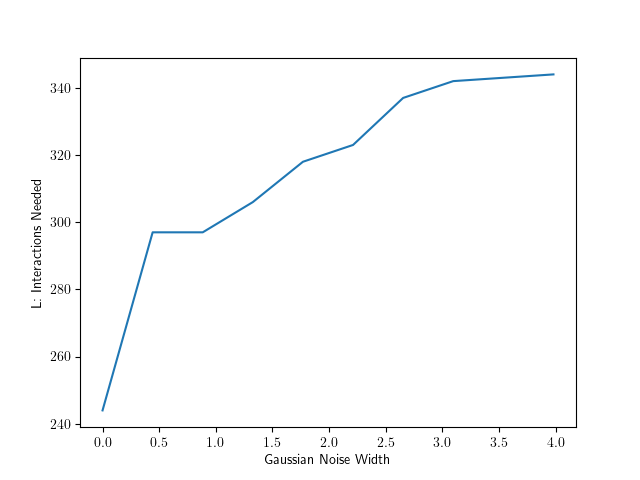
\includegraphics[width=0.475\linewidth]{numerics/data/h_chain_3_with_noise_2.png}
    \caption{Effects of noise added to exact spectrum sampling for Hydrogen chains, H2 on left and H3 on right. As we can see both tend to increase and then plateau. The parameters of these plots are $\beta = 1.0$, $\alpha = 0.01$, and $t = 150$ for H2 and $t = 200$ for H3.}
    \label{fig:h_chain_with_noise}
\end{figure}

\section{Conclusion - DEFCON 4} \label{sec:conclusion}

Thermal state preparation is likely to be a crucial preparation step for the simulation of quantum systems on digital quantum computers. We have presented an algorithm for this task that has an optimally minimal number of overhead ancilla qubits and compiles to remarkably simple circuits of just time independent Hamiltonian evolution of the unprocessed system Hamiltonian with no complicated filtering or rejection steps and no Fourier weighted jump operators of Linbladians. Our algorithm is based on relatively recent classical Monte Carlo techniques, specifically Hamiltonian Monte Carlo \cite{hoffman2011nouturnsampleradaptivelysetting} and the end result bears striking resemblance to the Repeated Interactions framework in open quantum systems \cite{prositto2025equilibrium}. In Hamiltonian Monte Carlo thermal states over a position coordinate $q$ is prepared by sampling momentum $p$ from the Boltzmann distribution for Gaussians $e^{-\beta p^2/2m}$ followed by time evolution. Classical Hamiltonian dynamics is enough to couple the position and momentum, leading to the Boltzmann distribution over $q$ with enough time and samples.

Our algorithm extends this procedure to quantum computers. Instead of adding in momentum variables, which is difficult to define for discrete quantum systems, we add in a single ancilla qubit prepared in the thermal state at the desired inverse temperature $\beta$. We do not have the luxury of classical Hamiltonian dynamics that would couple these two registers, so we add in a randomized interaction term to the Hamiltonian. After simulating the time dynamics of this system-ancilla pair and repeating multiple times we are able to thermalize the system to the same $\beta$.

In the classical regime it is well known that sharp gradients in the Hamiltonian require longer simulation time and more samples to converge. Our quantum algorithm has a much more subtle dependence on the structure of the Hamiltonian. As our single ancilla qubit only has one energy difference $\gamma$, we have to tune this energy difference to allow for energy to be siphoned off from the system into the ancilla. This would present a conundrum, as knowing spectral gaps is just as difficult as preparing ground states of arbitrary quantum Hamiltonians, but we are able to prove that our algorithm is robust to complete ignorance of these differences. We show that this ignorance comes at an asymptotic cost in the amount of resources needed to prepare the thermal state. We numerically verify this and show that as we add noise to the sampled eigenvalue differences the total runtime needed to thermalize increases. We posit that this behavior serves as a crucial entry point for heuristics about Hamiltonian spectra into thermal state preparation algorithms that has not been explicitly demonstrated in prior algorithms. It was our hope to analytically quantify the speedups gained as a function of the relative entropy between a heuristic guess for the eigenvalue differences and the true spectra, but our numeric evidence will have to suffice until future work can clarify this dependence.

We would like to make a few remarks on potential improvements for the analysis of this algorithm. As we have demonstrated numerically, our guaranteed analytic values of $\alpha$ and $t$ that lead to thermalization are drastically overestimated. We conjecture that this is due to our truncation of the weak-coupling expansion and demonstrate that taking $\alpha \propto 1/t$ and $t \propto 1/ \sqrt{\epsilon}$ drastically outperforms our analytically derived bounds of $\alpha \propto 1/t^3$. It is unclear to us how this may be shown analytically. It is also an open question of whether dynamically chosen values of $\alpha$ and $t$, such as having strong coupling and low time at the beginning and gradually decreasing $\alpha$ and increasing $t$, can outperform static $\alpha$ and $t$. We also suspect that the Markov relaxation theorem we used greatly overestimates the number of interactions needed. It remains to be seen if better Markov theory is needed or if the convergence time could be characterized based on the overlap of the initial state with the thermal state, which is a property that a few ground state preparation algorithms demonstrate. Our last remark for potential avenues for improving the analysis of this algorithm is whether different randomized interactions or even eigenvector heuristics can be beneficial. For example, in the harmonic oscillator if one has knowledge of the creation and annihilation operators $a^\dagger$ and $a$, could one simply use the interaction $a^\dagger \otimes (X + i Y) + a \otimes (X - i Y)$ instead of involving a randomized $G$ that relies on a Haar average? The last potential improvement to analyze this algorithm is to extend our spectral gap computations using perturbation theory. We are only able to compute the spectral gaps $\lambda_\star(\beta)$ in the limit of $\beta \to \infty$ but it should be possible to compute a perturbation on the order of $1/\beta$. This would give the runtime needed to prepare low-temperature thermal states as opposed to zero-temperature states.

Lastly we would like to speculate on possible applications of this routine to other quantum information processing tasks. The first question that arises is if this algorithm could be used in the training of quantum Boltzmann machines, which are essentially thermal states. It is an open question if our thermalizing techniques could be used to either train models or to generate output samples from an already trained model. Through the process of demonstrating that this algorithm prepares the system in the thermal state we have calculated the output of our channel for both the system and the environment registers, and for much larger environments than single qubits. We can turn this protocol on it's head and ask how much information about the system are these ancilla qubits carrying away with them? Preliminary explorations not included in this manuscript suggests that given knowledge about eigenvalue gaps one can use transition statistics in the ancilla qubits to infer what the inverse temperature $\beta$ is of the system, assuming the system is in a thermal state. Could this thermalizing procedure instead be used to develop a Bayesian model to update beliefs about Hamiltonian spectra and system temperatures? This would represent an interaction agnostic model for performing quantum thermometry or spectroscopy, which to our knowledge has not been developed yet. 

\bibliographystyle{unsrt}
\bibliography{bib}

\appendix 


\section{Technical Proofs - DEFCON 5} \label{sec:appendix}
\subsection{Sinc Bounds} \label{sec:appendix_sinc}

\begin{lemma}[Sinc Function Bounds] \label{lem:sinc_poly_approx}
    For $\sinc^2\left( \frac{x t}{2} \right)$ and $\delta_{\min}$ as defined in Eq. \eqref{eq:delta_min_def}, we will make significant use of the following bounds:
    \begin{align}
        |x| \ge \delta_{\min} \implies \sinc^2 \left( \frac{x t}{2} \right) &\le \frac{4}{\delta_{\min}^2 t^2} \label{eq:sinc_upper_bound} \\
        |x| \le \frac{\sqrt{2}}{t} \implies \sinc^2\left(\frac{x t}{2} \right) &\ge 1 - \frac{|x|^2 t^2}{2}. \label{eq:sinc_lower_bound}
\end{align}

\end{lemma}
\begin{proof}
    The first inequality is rather trivial
    \begin{align}
        \sinc^2 \left( \frac{x t}{2} \right) &= \frac{\sin^2 (x t /2)}{(x t / 2)^2} \le \frac{4}{x^2 t^2} \le \frac{4}{\delta_{\min}^2 t^2}.
    \end{align}
    The second involves a Taylor Series for $\sinc^2$, which we compute using the expression of $\sinc$ as $\sinc(x t/ 2) = \frac{\sin xt /2}{xt/2} = \int_0^1 \cos(sxt/2) ds$.  The first two derivatives can then be computed easily
    \begin{align}
        \frac{d \sinc^2(x t /2)}{dx} &= - t \int_0^1 \sin(sx) s ds \int_0^1 \cos(sx) ds \\
        \frac{d^2 \sinc^2(x t /2)}{dx^2} &= -t^2 / 2 \int_0^1 \cos(sx)s^2 ds \int_0^1 \cos(sx) ds + t^2 / 2 \int_0^1 \sin(sx) s ~ds \int_0^1 \sin(sx) s ~ds.
    \end{align}
    We can evaluate each of these derivatives about the origin using continuity of the derivatives along with the limits $\lim_{x \to 0} \cos(sx) = 1$ and $\lim_{x \to 0} \sin(sx) = 0$. We can now compute the mean-value version Taylor series as
    \begin{align}
        \sinc^2 \left(\frac{x t}{2} \right) &= \sinc^2(0) + x \frac{d}{dx} \sinc^2 \left(\frac{x t}{2} \right) \bigg|_{x = 0} + \frac{x^2}{2!} \frac{d^2}{dx^2} \sinc^2 \left(\frac{x t}{2} \right) \bigg|_{x = x_{\star}},
    \end{align}
    where $x_{\star} \in [0,1]$. 
    Plugging in $\sinc^2(0) = 1$ and $\frac{d\sinc^2(x t /2)}{dx}\big|_{x = 0} = 0$ then yields $|\sinc^2(xt/2) - 1| = \frac{|x|^2}{2} \abs{\frac{d^2\sinc^2(x t / 2)}{dx^2}\big|_{x = x_{\star}}}$. We make use of the rather simplistic bound
    \begin{align}
        \abs{\frac{d^2\sinc^2(sxt/2)}{dx^2}\bigg|_{x = x_{\star}} } &\leq t^2 / 2 \abs{\int_0^1 \cos(sx_{\star} t/ 2) s^2 ds \int_0^1 \cos(sx_{\star} t/ 2) ds} + t^2 /2 \abs{\int_0^1 \sin(sx_{\star} t/ 2) s ds \int_0^1 \sin(sx_{\star} t/ 2) s ds} \\
        &\leq t^2 / 2 \int_0^1 \abs{\cos(sx_{\star} t/2)} s^2 ds \int_0^1 \abs{\cos(sx_{\star} t /2 )} ds + t^2 / 2 \parens{\int_0^1 \abs{\sin(sx_{\star} t /2)} |s| ds}^2 \\
        &\leq t^2 / 2 \int_0^1 s^2 ds + t^2 / 2 \parens{\int_0^1 s ds}^2 \\
        &\leq t^2.
    \end{align}
    This yields the final inequality $|\sinc^2(x t /2 ) - 1| \leq \frac{|x|^2 t^2}{2}$ which yields Eq. \eqref{eq:sinc_lower_bound}.
\end{proof}


\subsection{Haar Integral Proofs} \label{sec:haar_integral_appendix}

In this section we present the more technical work needed to state our results in Section \ref{sec:weak_coupling}. Lemmas \ref{lem:two_heisenberg_interactions} and \ref{lem:sandwiched_interaction} are used to compute the effects of the randomized interactions in a form that are usable in the main result of Lemma \ref{lem:big_one}. Lemma \ref{lem:haar_two_moment} can be derived from Appendix C in \cite{brandao2021complexity}.
\begin{restatable}{lemma}{haar_two_moment} \label{lem:haar_two_moment}
    Let $\int (\cdot) dU$ denote the average distributed according to the Haar measure over $\dim$-dimensional unitary matrices $U$. Then for $\ket{i_1},\ket{i_2},\ldots,\ket{k_2}$ drawn from an orthonormal basis
    \begin{align}
        &\int \bra{i_1} U \ket{j_1} \bra{i_2} U \ket{j_2} \bra{k_1} U^\dagger \ket{l_1} ~ \bra{k_2} U^\dagger \ket{l_2} dU \nonumber \\
        &= ~\frac{1}{\dim^2 - 1} \parens{\delta_{i_1, l_1} \delta_{j_1, k_1} \delta_{i_2, l_2} \delta_{j_2, k_2} + \delta_{i_1, l_2} \delta_{j_1, k_2} \delta_{i_2, l_1} \delta_{j_2, k_1}} \nonumber \\
        &\quad - \frac{1}{\dim(\dim^2 - 1)} \parens{\delta_{i_1, l_2} \delta_{j_1, k_1} \delta_{i_2, l_1} \delta_{j_2, k_2} + \delta_{i_1, l_1} \delta_{j_1, k_2} \delta_{i_2, l_2} \delta_{j_2, k_1}}. \label{eq:haar_two_moment_integral}
    \end{align}
\end{restatable}

\begin{lemma} \label{lem:two_heisenberg_interactions}
    Let $G(t)$ denote the Heisenberg evolved random interaction $G(t) = e^{iHt} G e^{-iHt}$ for a total Hamiltonian $H$. After averaging over the interaction measure the product $G(x) G(y)$ can be computed as
    \begin{equation}
        \int G(x) G(y) dG = \frac{1}{\dim + 1} \parens{\sum_{(i,j),(k,l)} e^{i \Delta(i,j|k,l) (x-y)} \ketbra{i,j}{i,j} + \identity}.
    \end{equation}
\end{lemma}
\begin{proof}
The overall structure of this proof is to evaluate the product in the Hamiltonian eigenbasis and split the product into three factors: a phase contribution from the time evolution, a Haar integral from the eigenvalues of the random interaction, and the eigenvalue contribution of the random interaction. Since this involves the use of multiple indices, it will greatly simplify the proof to use a single index over the total Hilbert space $\hilb$ as opposed to two indices over $\hilb_S \otimes \hilb_E$. For example, the index $a$ should be thought of as a pair $(a_s, a_e)$, and functions $\lambda(a)$ should be thought of as $\lambda(a_s, a_e)$. Once the final form of the expression is reached we will substitute in pairs of indices for easier use of the lemma in other places.
    \begin{align}
        \int G(x) G(y) dG &= \int e^{+i H x} U_G D U_G^\dagger e^{-i H x} e^{+i H y} U_G D U_G^\dagger e^{-i H y} dU_G ~dD \\
        &= \int \bigg[\sum_a e^{+i \lambda(a)x}\ketbra{a}{a}  U_G \sum_b D(b)\ketbra{b}{b} U_G^\dagger \nonumber \\
        &\quad \sum_c e^{-i \lambda(c) (x - y)} \ketbra{c}{c} U_G \sum_d D(d)\ketbra{d}{d} U_G^\dagger \sum_e e^{-i \lambda(e) y} \ketbra{e}{e} \bigg] dU_G ~dD\\
        &=\sum_{a,b,c,d,e} \ketbra{a}{e} e^{-i (\lambda(c) - \lambda(a))x} e^{-i (\lambda(e) - \lambda(c))y} \nonumber \\
        &\quad \times \int \bra{a} U_G \ket{b} \bra{c} U_G \ket{d} \bra{b} U_G^{\dagger} \ket{c} \bra{d} U_G^\dagger \ket{e} dU_G \int D(b) D(d) dD \\
        &=  \sum_{a, b, c, d, e} \delta_{bd} \ketbra{a}{e} e^{-i (\lambda(c) - \lambda(a))x} e^{-i (\lambda(e) - \lambda(c))y} \nonumber \\
        &\quad \times \int \bra{a} U_G \ket{b} \bra{c} U_G \ket{d} \bra{b} U_G^{\dagger} \ket{c} \bra{d} U_G^\dagger \ket{e} dU_G. \\
    \end{align}
    Now the summation over $d$ fixes $d=b$ and we use Lemma \ref{lem:haar_two_moment} to compute the Haar integral, which simplifies greatly due to the repeated $b$ index. Plugging the result into the above yields the following
    \begin{align}
        &= \frac{1}{\dim^2 - 1} \sum_{a, b, c, e} \ketbra{a}{e} e^{-i (\lambda(c) - \lambda(a))x} e^{-i (\lambda(e) - \lambda(c))y} \parens{\delta_{ac} \delta_{ce} + \delta_{ae} - \frac{1}{\dim} \parens{\delta_{ac} \delta_{ce} + \delta_{ae}}}  \\
        &= \frac{1}{\dim^2 - 1} \parens{1 - \frac{1}{\dim}} \sum_{a, b, c, e} \ketbra{a}{e} e^{-i (\lambda(c) - \lambda(a))x} e^{-i (\lambda(e) - \lambda(c))y} \delta_{ae} (1 + \delta_{ac}) \\
        &= \frac{1}{\dim^2 - 1} \parens{1 - \frac{1}{\dim}} \sum_{a, b, c} \ketbra{a}{a} e^{i (\lambda(a) - \lambda(c))(x-y)} (1 + \delta_{ac}) \\
        &= \frac{1 \parens{\dim - 1}}{\dim^2 - 1} \sum_{a,c} \ketbra{a}{a} e^{i (\lambda(a) - \lambda(c))(x - y)} (1 + \delta_{ac}) \\
        &= \frac{1}{\dim + 1} \parens{\sum_{a,c} e^{i (\lambda(a) - \lambda(c))(x-y)} \ketbra{a}{a} + \identity}.
    \end{align}
    Reindexing by $a \mapsto i,j$, $c \mapsto k,l$, and plugging in the definition of $\Delta$ yields the statement of the lemma.
\end{proof}


\begin{lemma} \label{lem:sandwiched_interaction}
    Given two Heisenberg evolved random interactions, $G(x)$ and $G(y)$, we compute their action on an outer-product $\ketbra{i,j}{k,l}$ as
    \begin{equation}
        \int G(x) \ketbra{i,j}{k,l} G(y) ~dG = \frac{1}{\dim + 1} \parens{\ketbra{i,j}{k,l} + \braket{i,j}{k,l} \sum_{m,n} e^{i \Delta(m,n | i,j) (x-y)} \ketbra{m,n}{m,n}}
    \end{equation}
\end{lemma}
\begin{proof}
This proof is structured the same as Lemma \ref{lem:two_heisenberg_interactions} and similarly we will use a single index of the total Hilbert space $\hilb$ and switch to two indices to match the rest of the exposition.
    \begin{align}
        \int G(x) \ketbra{a}{b} G(y) dG &=  \int e^{i H x} U_G D U_G^{\dagger} e^{-i H x} \ketbra{a}{b} e^{i H y} U_G D U_G^\dagger e^{-i H y} ~dG \\
        &= \sum_{c, d, e, f} e^{i (\lambda(c) - \lambda(a))x} e^{i (\lambda(b) - \lambda(f))y} \nonumber \\
        &\quad \times \int \ketbra{c}{c} U_G D(d) \ketbra{d}{d} U_G^\dagger \ketbra{a}{b} U_G D(e) \ketbra{e}{e} U_G^\dagger \ketbra{f}{f} dG \\
        &= \sum_{c, d, e, f}  e^{i (\lambda(c) - \lambda(a))x} e^{i (\lambda(b) - \lambda(f))y} \ketbra{c}{f} \nonumber \\
        &\quad \times \int D(d) D(e) dD \int \bra{c} U_G \ket{d} \bra{b} U_G \ket{e} \bra{d} U_G^\dagger \ket{a} \bra{e} U_G^\dagger \ket{f} dU_G \\
        &=  \sum_{c,d,f} e^{i (\lambda(c) - \lambda(a))x} e^{i (\lambda(b) - \lambda(f))y} \ketbra{c}{f} \nonumber \\ 
        &\quad \times \int \bra{c} U_G \ket{d} \bra{b} U_G \ket{d} \bra{a} \overline{U_G} \ket{d} \bra{f} \overline{U_G} \ket{d} dU_G \\
        &= \frac{1}{\dim^2 - 1} \sum_{c,d,f} e^{i (\lambda(c) - \lambda(a))x} e^{i (\lambda(b) - \lambda(f))y} \ketbra{c}{f} (\delta_{ca} \delta_{bf} + \delta_{cf}\delta_{ab})\parens{1 - \frac{1}{\dim}} \\
        &= \frac{1}{\dim + 1} \sum_{c,f} e^{i (\lambda(c) - \lambda(a))x} e^{i (\lambda(b) - \lambda(f))y} \ketbra{c}{f} (\delta_{ca} \delta_{bf} + \delta_{cf}\delta_{ab}) \\
        &= \frac{1}{\dim + 1} \parens{\ketbra{a}{b} + \delta_{ab} \sum_{c} e^{i(\lambda(c) - \lambda(a))(x-y)} \ketbra{c}{c} }.
    \end{align}
    Now re-indexing by $a \mapsto (i,j)$, $b \mapsto (k,l)$ and $c \mapsto (m,n)$ results in the expression given in the statement of the lemma.
\end{proof}


\secondOrderChannelHaar*
\begin{proof}
To start we would like to note that we will use a single index notation to refer to the joint system-environment eigenbasis during this proof to help shorten the already lengthy expressions. We will convert back to a double index notation to match the statement of the theorem. We start from the expression for the first derivative of the channel $\frac{\partial}{\partial \alpha} \Phi_G(\rho_S)$ given by Eq. \eqref{eq:first_order_alpha_derivative}. To take the second derivative there are six factors involving $\alpha$, so we will end up with six terms. We repeat Eq. \eqref{eq:first_order_alpha_derivative} below, add a derivative, and label each factor containing an $\alpha$ for easier computation
\begin{align}
    \frac{\partial^2}{\partial \alpha^2} \Phi_G(\rho_S) =& \frac{\partial}{\partial \alpha} \parens{\int_{0}^{1} \underset{\substack{\downarrow \\ (A)}}{e^{i s (H+\alpha G)t}} (i t G) \underset{\substack{\downarrow \\ (B)}}{e^{i (1-s) (H+\alpha G)t}} ds ~ \rho \underset{\substack{\downarrow \\ (C)}}{e^{-i(H+\alpha G)t}} } \nonumber \\
    &~ ~+\frac{\partial}{\partial \alpha} \parens{ \underset{\substack{\downarrow \\ (D)} }{e^{i(H+\alpha G)t}} \rho \int_{0}^1 \underset{\substack{\downarrow \\ (E)} }{e^{-i s (H+\alpha G) t} } (- i t G) \underset{\substack{\downarrow \\ (F)}}{e^{-i (1-s) (H+\alpha G)t}} ds }. \label{eq:second_derivative_labels}
\end{align}
Our goal is to get each of these terms in a form in which we can use either Lemma \ref{lem:two_heisenberg_interactions} or \ref{lem:sandwiched_interaction}. 
\begin{align}
    (A) &=i t\int_0^1 \parens{\frac{\partial}{\partial \alpha} e^{i s_1 (H+ \alpha G)t}} G e^{i(1-s_1)(H+\alpha G)t} ds_1 \rho e^{-i (H+\alpha G)t} \bigg|_{\alpha=0} \\
    &= (it)^2 \int_0^1 \parens{\int_0^1 e^{i s_1 s_2 (H+\alpha G)t} s_1 G e^{i s_1 (1-s_2) (H+\alpha G)t} ds_2} G e^{i(1-s_1) (H+\alpha G)t} ds_1 \rho e^{-i(H+\alpha G) t} \bigg|_{\alpha=0} \label{eq:second_order_deriv_intermediate_a}\\
    &= -t^2 \int_0^1 \int_0^1 e^{i s_1 s_2 H t} G e^{-i s_1 s_2 H t} e^{i s_1 H t} G e^{-i s_1 H t} s_1 ds_1 ds_2 e^{i H t} \rho e^{-i H t} \\
    &= -t^2 \int_0^1 \int_0^1 G(s_1 s_2 t) G(s_1 t) s_1 ds_1 ds_2 \rho(t). \label{eq:second_deriv_alpha_first_term}
\end{align}

\begin{align}
    (B) &= it \int_0^1 e^{i s_1 (H + \alpha G)t} G \frac{\partial}{\partial \alpha}\parens{e^{i(1-s_1)(H + \alpha G)t}} ds_1 \rho e^{-i(H + \alpha G) t} \bigg|_{\alpha = 0} \\
    &= (it)^2 \int_0^1 e^{i s_1 (H + \alpha G)t} G \parens{\int_0^1 e^{i(1-s_1)s_2 (H + \alpha G)t} (1-s_1) G e^{i(1 - s_1)(1 - s_2)(H + \alpha G)t} ds_2} ds_1 ~ \rho e^{-i ( H + \alpha G)t} \bigg|_{\alpha = 0} \\
    &= -t^2 \int_0^1 \int_0^1 e^{i s_1 H t} G e^{i(1-s_1)s_2 H t} G e^{i(1-s_1)(1-s_2) H t} (1-s_1) ds_1 ds_2 ~ \rho e^{-i H t}\\ 
    &= -t^2 \int_0^1 \int_0^1 e^{i s_1 H t} G e^{-i s_1 H t} e^{i(s_1 + s_2 - s_1 s_2) H t} G e^{-i (s_1 + s_2 - s_1 s_2) H t} (1-s_1) ds_1 ds_2 ~ \rho(t) \\
    &= -t^2 \int_0^1 \int_0^1 G(s_1 t) G((s_1 + s_2 - s_1 s_2)t) (1-s_1) ds_1 ds_2 ~ \rho(t)
\end{align}

\begin{align}
    (C) &= it \int_0^1 e^{i s (H + \alpha G)t} G e^{i(1-s) (H + \alpha G) t} ds ~\rho ~ \frac{\partial}{\partial \alpha} \parens{ e^{-i (H + \alpha G) t} } \bigg|_{\alpha = 0} \\
    &= (i t) (-it) \int_0^1 e^{i s (H + \alpha G)t} G e^{i (1 - s) (H + \alpha G)t} ds ~ \rho ~ \parens{ \int_0^1 e^{-i s (H + \alpha G)t} G e^{-i (1- s) ( H + \alpha G)t } ds}\bigg|_{\alpha = 0} \\
    &= + t^2 \parens{\int_0^1 e^{i s H t} G e^{-i s H t} ds} e^{i H t} \rho e^{-i H t} \parens{\int_0^1 e^{i (1-s) H t} G e^{-i (1-s) H t} ds} \\
    &= + t^2 \int_0^1 G(st) ds ~ \rho(t) \int_0^1 G((1-s)t) ds
\end{align}

\begin{align}
    (D) &= (-it) \frac{\partial}{\partial \alpha} \parens{e^{i(H + \alpha G)t}} \rho \int_0^1 e^{-i s (H + \alpha G)t} G e^{-i (1-s)(H + \alpha G)t} ds \bigg|_{\alpha = 0} \\
    &= t^2 \parens{\int_0^1 e^{i s (H+ \alpha G)t} G e^{i (1-s) (H + \alpha G)t}ds} \rho \int_0^1 e^{-i s (H + \alpha G)t} G e^{-i (1-s)(H + \alpha G)t} ds \bigg|_{\alpha = 0} \\
    &=  t^2 \int_0^1 e^{i s H t} G e^{-i s H t} ds ~\rho(t) \int_0^1 e^{i (1-s) H t} G e^{-i (1-s) H t} ds \\
    &= t^2 \int_0^1 G(st) ds ~ \rho(t) ~ \int_0^1 G((1-s)t) ds
\end{align}

\begin{align}
    (E) &= (-it) e^{i (H+ \alpha G) t} ~ \rho ~\int_0^1 \frac{\partial}{\partial \alpha} \parens{e^{-i s_1 (H + \alpha G)t}} G e^{-i (1-s_1)(H + \alpha G)t} ds_1 \bigg|_{\alpha = 0} \\
    &= - t^2 e^{i(H + \alpha G)t} ~ \rho ~\int_0^1 \parens{\int_0^1 e^{-i s_1 s_2 (H + \alpha G) t} (s_1 G) e^{-i s_1 (1-s_2) (H + \alpha G)t} ds_2} G e^{-i(1-s_1)(H + \alpha G)t} ds_1 \bigg|_{\alpha = 0} \\
    &= -t^2 e^{i H t} \rho e^{-i H t} \int_0^1 \int_0^1 e^{i (1 - s_1 s_2) H t} G e^{-i (s_1 - s_1 s_2)H t} G e^{-i (1-s_1)H t} s_1 ds_1 ds_2 \\
    &= -t^2 \rho(t) \int_0^1 \int_0^1 G((1- s_1 s_2) t) G((1-s_1)t) s_1 ds_1 ds_2
\end{align}

\begin{align}
    (F) &= (-it) e^{i(H + \alpha G) t} \rho \int_0^1 e^{-i s_1 ( H + \alpha G) t} G \frac{\partial}{\partial \alpha} \parens{ e^{-i (1-s_1) ( H +\alpha G)t}} ds_1 \bigg|_{\alpha = 0} \\
    &= (-it)^2 e^{i (H + \alpha G)t} \rho \int_0^1 e^{-i s_1 (H + \alpha G)t} G \parens{\int_0^1 e^{-i(1-s_1) s_2 (H + \alpha G)t} (1-s_1) G e^{-i(1-s_1) (1-s_2) (H + \alpha G) t} ds_2} ds_1 \bigg|_{\alpha = 0} \\
    &= -t^2 e^{-i H t} \rho e^{-i H t} \int_0^1 \int_0^1 e^{i (1- s_1) H t} G e^{-i (1-s_1) H t} e^{i (1-s_1)(1-s_2) H t} G e^{-i(1-s_1)(1-s_2) H t} (1-s_1) ds_1 ds_2 \\
    &= -t^2 \rho(t) \int_0^1 \int_0^1 G((1-s_1)t) G((1-s_1)(1 - s_2) t) (1-s_1)ds_1 ds_2
\end{align}

Now our goal is to compute the effects of averaging over the interaction $G$ on the above terms, starting with $(A)$. As this involves a lot of index manipulations, similarly to the proofs of Lemmas \ref{lem:two_heisenberg_interactions} and \ref{lem:sandwiched_interaction} we will use a single index for the total system-environment Hilbert space and switch back to a double index to state the results. We will make heavy use of Lemma \ref{lem:two_heisenberg_interactions}.
\begin{align}
    \int (A) dG &= -t^2 \int_0^1 \int_0^1 \int G(s_1 s_2 t) G(s_1 t) dG s_1 ds_1 ds_2 \rho(t) \\
    &= \frac{-t^2 }{\dim + 1} \int_0^1 \int_0^1 \parens{\sum_{i,j} e^{i (\lambda(i) - \lambda(j)) (s_1 s_2 t - s_1 t)} \ketbra{i}{i} + \identity} s_1 ds_1 ds_2 \rho(t) \\
    &= \frac{- t^2 }{\dim + 1} \parens{\sum_{i} \sum_{j : \lambda(i) \neq \lambda(j)} \int_0^1 \int_0^1 e^{i(\lambda(i) - \lambda(j))t (s_1 s_2 - s_1)} s_1 ds_1 ds_2 \ketbra{i}{i} + \sum_{i} \sum_{j : \lambda(i) = \lambda(j)}\frac{1}{2} \ketbra{i}{i} + \frac{1}{2} \identity} \rho(t) \\
    &= \frac{- t^2 }{\dim + 1} \parens{\sum_i \sum_{j : \lambda(i) \neq \lambda(j)} \frac{1 - i (\lambda(i) - \lambda(j))t - e^{-i (\lambda(i) - \lambda(j))t}}{t^2 (\lambda(i) - \lambda(j))^2} \ketbra{i}{i} + \frac{1}{2} \sum_{i} (\eta(i) + 1) \ketbra{i}{i} } \rho(t) \\
    &= \frac{- 1}{\dim + 1}\parens{\sum_{i} \sum_{j: \Delta_{ij} \neq 0} \frac{1 - i \Delta_{ij}t - e^{-i \Delta_{ij} t}}{\Delta_{ij}^2} \ketbra{i}{i} + \frac{t^2}{2} \sum_{i} (\eta(i) + 1)\ketbra{i}{i} } \rho(t)
\end{align}

We can similarly compute the averaged $(B)$ term:
\begin{align}
    \int (B) dG &= -t^2 \int_0^1 \int_0^1 \int G(s_1 t) G((s_1 + s_2 - s_1 s_2) t) dG (1-s_1) ds_1 ds_2 ~ \rho(t) \\
    &= \frac{- t^2 }{\dim + 1} \int_0^1 \int_0^1 \parens{\sum_{i,j} e^{i (\lambda(i) - \lambda(j))(s_1 s_2 - s_2) t} \ketbra{i}{i} + \identity} (1 -s_1) ds_1 ds_2 \rho \\
    &= \frac{- t^2 }{\dim + 1} \parens{\sum_{i} \sum_{j : \lambda(i) \neq \lambda(j)} \int_0^1 \int_0^1 e^{i(\lambda(i) - \lambda(j))t (s_1 s_2 - s_2)} (1 - s_1) ds_1 ds_2 \ketbra{i}{i} + \sum_{i} \sum_{j : \lambda(i) = \lambda(j)}\frac{1}{2} \ketbra{i}{i} + \frac{1}{2} \identity} \rho(t) \\
    &= \frac{- t^2 }{\dim + 1} \parens{\sum_i \sum_{j : \lambda(i) \neq \lambda(j)} \frac{1 - i (\lambda(i) - \lambda(j))t - e^{-i (\lambda(i) - \lambda(j))t}}{t^2 (\lambda(i) - \lambda(j))^2} \ketbra{i}{i} + \frac{1}{2} \sum_{i} (\eta(i) + 1) \ketbra{i}{i} } \rho(t) \\
    &= \frac{-1}{\dim + 1}\parens{\sum_{i} \sum_{j: \Delta_{ij} \neq 0} \frac{1 - i \Delta_{ij}t - e^{-i \Delta_{ij} t}}{\Delta_{ij}^2} \ketbra{i}{i} + \frac{t^2}{2} \sum_{i} (\eta(i) + 1)\ketbra{i}{i} } \rho(t),
\end{align}
which we note is identical to $\int (A) dG$. As terms $(C)$ and $(D)$ involve a different method of computation we skip them for now and compute $(E)$ and $(F)$. 
\begin{align}
    \int (E) dG &= -t^2 \rho(t) \int_0^1 \int_0^1 \int G((1- s_1 s_2) t) G((1-s_1)t) dG s_1 ds_1 ds_2 \\
    &= \frac{- t^2}{\dim + 1} \rho(t) \int_0^1 \int_0^1 \parens{\sum_{i,j} e^{i(\lambda(i) - \lambda(j)) t (s_1 - s_1 s_2)} \ketbra{i}{i} + \identity } s_1 ds_1 ds_2 \\
    &= \frac{- t^2}{\dim + 1} \rho(t) \parens{\sum_i \sum_{j : \lambda(i) \neq \lambda(j)} \frac{1 + i (\lambda(i) - \lambda(j))t - e^{i(\lambda(i) - \lambda(j))t}}{t^2 (\lambda(i) - \lambda(j))^2}\ketbra{i}{i} + \frac{1}{2} \sum_{i} (\eta(i) + 1 )\ketbra{i}{i}} \\
    &= \frac{- 1}{\dim + 1} \rho(t) \parens{\sum_i \sum_{j: (\Delta_{ij} \neq 0)} \frac{1 + i \Delta_{ij}t - e^{i\Delta_{ij}t}}{\Delta_{ij}^2} \ketbra{i}{i} + \frac{t^2}{2}\sum_i (\eta(i) + 1) \ketbra{i}{i}}.
\end{align}
Computing $(F)$ yields
\begin{align}
    \int (F) dG &= -t^2 \rho(t) \int_0^1 \int_0^1 \int G((1-s_1)t) G((1-s_1)(1 - s_2) t) dG (1-s_1)ds_1 ds_2 \\
    &= \frac{- t^2 \sigma ^2}{\dim + 1} \rho(t) \int_0^1 \int_0^1 \parens{\sum_{i,j} e^{i(\lambda(i) - \lambda(j))t (s_2 - s_1 s_2)}\ketbra{i}{i} + \identity} (1-s_1) ds_1 ds_2 \\
    &= \frac{- t^2 }{\dim + 1} \rho(t) \parens{\sum_{i} \sum_{j : \lambda(i) \neq \lambda(j)} \frac{1 + i (\lambda(i) - \lambda(j))t - e^{i (\lambda(i) - \lambda(j))t}}{t^2 (\lambda(i) - \lambda(j))^2} \ketbra{i}{i} +\frac{1}{2} \sum_{i} (\eta(i) + 1) \ketbra{i}{i}} \\
    &= \frac{- 1}{\dim + 1} \rho(t) \parens{\sum_i \sum_{j: (\Delta_{ij} \neq 0)} \frac{1 + i \Delta_{ij}t - e^{i\Delta_{ij}t}}{\Delta_{ij}^2} \ketbra{i}{i} + \frac{t^2}{2}\sum_i (\eta(i) + 1) \ketbra{i}{i}}
\end{align}
 which is identical to $\int (E) dG$.

 The last two terms $(C) = (D)$ are computed as follows:
 \begin{align}
     \int (C) dG &= t^2 \int_0^1 \int_0^1 \int G(s_1 t) \rho(t) G((1-s_2)t) ~dG ~ ds_1 ds_2 \\
     &= t^2 \sum_{i,j} \rho_{ij} e^{i(\lambda(i) - \lambda(j))t} \int_0^1 \int_0^1 \int G(s_1 t) \ketbra{i}{j} G((1-s_2)t) ~ dG ~ ds_1 ds_2 \\
     &= \frac{ t^2}{\dim + 1} \sum_{i,j} \rho_{ij} e^{i(\lambda(i) - \lambda(j))t} \parens{ \ketbra{i}{j} + \delta_{ij} \sum_{a} \int_0^1 \int_0^1 e^{i(\lambda(a) - \lambda(i))(s_1 + s_2 - 1)t} ds_1 ds_2 \ketbra{a}{a}} \\
     &= \frac{ t^2}{\dim + 1} \sum_{i,j} \rho_{ij} e^{i \Delta_{ij} t} \parens{\ketbra{i}{j} + \delta_{ij} \sum_{a : \Delta_{ai} \neq 0} \frac{2( 1- \cos (\Delta_{ai} t))}{\Delta_{ai}^2 t^2} \ketbra{a}{a} + \delta_{ij} \sum_{a : \Delta_{ai} = 0} \ketbra{a}{a}}
 \end{align}

 We can now combine each of these terms to offer the full picture of the output of the channel to second order. We make two modifications to the results from each sum: first, we will switch to double index notation to make for easier use in other areas, and secondly we let $\rho = \ketbra{i,j}{k,l}$. We note that the first term in the following equation is provided by $(A) + (B)$, the second through $(E) + (F)$, and the last two through $(C) + (D)$. 
 \begin{align}
     &\int \frac{\partial^2}{\partial \alpha^2} \Phi_G(\ketbra{i,j}{k,l})\bigg|_{\alpha = 0} dG \\
     &= -\frac{2  e^{i \Delta(i,j|k,l) t}}{\dim + 1} \bigg(\sum_{(a,b): \Delta(i,j|a,b) \neq 0} \frac{1 - i \Delta(i,j|a,b)t - e^{-i \Delta(i,j|a,b) t}}{\Delta(i,j|a,b)^2} \nonumber \\
     &~+ \sum_{(a,b): \Delta(k,l|a,b) \neq 0} \frac{1 + i \Delta(k,l|a,b) t - e^{i \Delta(k,l|a,b) t}}{\Delta(k,l|a,b)^2} + \frac{t^2}{2}(\eta(i,j) + \eta(k,l)) \bigg) \ketbra{i,j}{k,l} \nonumber \\
    &~ +\delta_{i,k} \delta_{j,l} \frac{2 e^{i \Delta(i,j|k,l)t}}{\dim+1} \parens{ \sum_{(a,b): \Delta(i,j|a,b) \neq 0 } \frac{2(1- \cos (\Delta(i,j|a,b)t))}{\Delta(i,j|a,b)^2} \ketbra{a,b}{a,b} + t^2 \sum_{(a,b) : \Delta(i,j|a,b) = 0} \ketbra{a,b}{a,b}} \label{eq:second_order_output}
 \end{align}
The last step we need is to use the half angle formula to change the cosine to a sine
\begin{align}
    \frac{2(1 - \cos(\Delta(i,j| a,b)t)}{\Delta(i,j|a,b)^2} &= \frac{2\left( 1 - \left(1 - 2 \sin^2\left(\frac{\Delta(i,j|a,b)t}{2} \right) \right) \right)}{\Delta(i,j|a,b)^2} \label{eq:trig_start} \\
    &= t^2 \frac{\sin^2 \left(\frac{\Delta(i,j|a,b) t}{2} \right)}{\frac{\Delta(i,j|a,b)^2 t^2}{4}} \\
    &= t^2 \sinc^2 \left(\frac{\Delta(i,j|a,b) t}{2 } \right), \label{eq:trig_end}
\end{align}
which yields the statement.


We can compute these by plugging in to Eq. \eqref{eq:el_gigante} again, which yields
\begin{align}s
&\int \bra{i', j'} \mathcal{T} \left( \ketbra{i, j}{i, j} \right) \ket{i', j'} ~dG = \begin{cases}        
\widetilde{\alpha}^2 \sinc^2(\Delta(i,j | i', j') t /2) & (i, j) \neq (i', j') \\
            - \widetilde{\alpha}^2 \sum_{(a,b) \neq (i, j)} \sinc^2(\Delta(a,b|i,j) t / 2) & (i,j) = (i', j')
        \end{cases}. \label{eq:system_environment_transitions}
    \end{align}
    The $(i, j) \neq (i', j')$ case should be apparent, the first term with the coherence factors $\chi$ are zero and the second term is what remains. The $(i,j) = (i', j')$ case can be seen as follows. For the first term we have
    \begin{align}
        - \frac{\alpha^2 e^{i \Delta(i,j| i,j) t}}{\dim + 1}\left(\chi(i,j) + \chi(i,j)^* + \frac{t^2}{2}(\eta(i,j) + \eta(i,j) \right) \ketbra{i,j}{i,j}.
    \end{align}
    We first compute the sum $\chi(i,j) + \chi(i,j)^*$ as
    \begin{align}
        \chi(i,j) + \chi(i,j)^* &= \sum_{a,b: \Delta(i,j,|a,b) \neq 0} \frac{1 - i \Delta(i,j|a,b)t - e^{-i \Delta(i,j|a,b) t}}{\Delta(i,j|a,b)^2} \nonumber\\
&\quad+ \sum_{a,b: \Delta(i,j,|a,b) \neq 0} \frac{1 + i \Delta(i,j|a,b)t - e^{+i \Delta(i,j|a,b) t}}{\Delta(i,j|a,b)^2} \\
    &= \sum_{a,b: \Delta(i,j| a,b) \neq 0} \frac{2 - e^{-i \Delta(i,j| a,b) t} - e^{+i \Delta(i,j| a,b) t}}{\Delta(i,j|a,b)^2} \\
    &= \sum_{a,b: \Delta(i,j| a,b) \neq 0} t^2 \sinc^2 \left( \frac{\Delta(i,j| a,b) t}{2} \right),
    \end{align}
    where the last step follows from a trigonometric identity (see Eqs. \eqref{eq:trig_start} - \eqref{eq:trig_end} in Appendix \ref{sec:haar_integral_appendix} for details). Since $\sinc(0) = 1$ the $\eta(i,j)$ term can be expressed as $\eta(i,j) = \sum_{a,b : \Delta(i,j|a,b) = 0} \sinc^2 \left( \frac{\Delta(i,j| a,b) t}{2} \right)$. Plugging this into Eq. \eqref{eq:el_gigante} gives
    \begin{align}
        &\int \bra{i,j} \mathcal{T} (\ketbra{i,j}{i,j}) \ket{i,j} dG \\
        &= \bra{i,j} \left(-\frac{\alpha^2 t^2}{\dim + 1} \sum_{a,b} \sinc^2 \left( \frac{\Delta(i,j| a,b) t}{2} \right) \ketbra{i,j}{i,j} + \sum_{a,b} \sinc^2\left( \frac{\Delta(i,j | a,b)t}{2} \right) \ketbra{a,b}{a,b} \right) \ket{i,j} \\
        &= -\frac{\alpha^2 t^2}{\dim + 1} \sum_{(a,b) \neq (i,j)} \sinc^2 \left( \frac{\Delta(i,j| a,b) t}{2} \right).
    \end{align}
    As a by-product of this computation we have just shown that $\trace{\mathcal{T}(\rho)} = 0$ and that our mapping is trace preserving to $\bigo{\alpha^2}$.
\end{proof}

\subsection{Weak-Coupling Remainder Bound} \label{sec:weak_coupling_remainder_bound}

\begin{proof}[Proof of Theorem~\ref{thm:remainder_bound}]
First we note that although $R_{\Phi}(\rho) = \frac{\alpha^3}{6} \partial_{\alpha}^3 \Phi(\rho)\big|_{\alpha = \alpha_{\star}}$ for a specific $ \alpha_{\star} > 0$ our proof will hold for any $\alpha_{\star}$. To compute the trace norm we will use the triangle inequality, unitary invariance of the Sch\"{a}tten norms, and submultiplicativity. To start,
\begin{align}
    \|\partial_\alpha^3 \Phi(\rho) \|_1 &= \left\| \frac{\partial^3}{\partial \alpha^3} {\rm Tr}_{H_E} \int e^{i(H+\alpha G)t} \rho_S \otimes \rho_E e^{-i(H+\alpha G)t} dG \bigg|_{\alpha = \alpha_{\star}} \right\|_1 \nonumber\\
    &= \left\| \frac{\partial^3}{\partial \alpha^3} {\rm Tr}_{H_E} \int e^{i(H+\alpha G)t} \rho_S \otimes \rho_E e^{-i(H+\alpha G)t} dG \bigg|_{\alpha = \alpha_{\star}} \right\|_1 \nonumber\\
    &\le    \int \left\|{\rm Tr}_{H_E}\frac{\partial^3}{\partial \alpha^3}\left( e^{i(H+\alpha G)t} \rho_S \otimes \rho_E e^{-i(H+\alpha G)t}\right) \bigg|_{\alpha = \alpha_{\star}} \right\|_1 dG.\label{eq:3derivBd}
\end{align}
To proceed, Proposition 1 of \cite{rastegin2012relations} allows us to eliminate the partial trace using the relation
$\norm{\partrace{\hilb_E}{X}}_{1} \le \norm{X}_{\dim_E} \le \norm{X}_1$. Further we use the decomposition of the second derivatives from the proof of Lemma \ref{lem:big_one}, specifically  Eq. \eqref{eq:second_derivative_labels} for the definition of each term, as $\partial_{\alpha}^2 \Phi_G = (A) + (B) + (C) + (D) +(E) + (F)$. This gives the following 
\begin{align}
    \norm{R_{\Phi}}_1 \le \frac{\alpha^3}{6} &\int \norm{\partial_{\alpha}((A) + (B) + (C) + (D) +(E) + (F)) \big|_{\alpha = \alpha_{\star}} }_1 dG \\
    &\le \frac{\alpha^3}{6} \int \norm{\partial_{\alpha}(A)\big|_{\alpha = \alpha_{\star}} }_1 + \norm{\partial_{\alpha}(B) \big|_{\alpha = \alpha_{\star}} }_1 + \ldots + \norm{\partial_{\alpha}(F) \big|_{\alpha = \alpha_{\star}} }_1 dG
\end{align}
We will demonstrate how this can be computed for the first term $\partial_{\alpha}(A)$. Using Eq. \ref{eq:second_deriv_alpha_first_term}
\begin{align}
\partial_{\alpha} (A) &= -t^2 \partial_{\alpha} \int_0^1 \int_0^1 e^{i s_1 s_2 (H+\alpha G)t} G e^{i s_1 (1-s_2) (H+\alpha G)t} G e^{i(1-s_1) (H+\alpha G)t} \rho e^{-i(H+\alpha G) t}   s_1 ~ds_1 ds_2.
\end{align}
Due to the multiplication rule the resulting derivative will have 4 terms that each need one application of Duhamel's formula. We will show one of these terms, starting with the leftmost one
\begin{align}
    -t^2  &\int_0^1 \int_0^1 \partial_{\alpha} \left( e^{i s_1 s_2 (H+\alpha G)t} \right) G e^{i s_1 (1-s_2) (H+\alpha G)t} G e^{i(1-s_1) (H+\alpha G)t} \rho e^{-i(H+\alpha G) t}   s_1 ~ds_1 ds_2 \\
    = - i t^3  &\int_0^1 \int_0^1 \int_0^1 \left( e^{i s_1 s_2 s_3 (H+\alpha G)t} G e^{i s_1 s_2 (1 - s_3) (H+\alpha G)t} \right)\nonumber\\
    &\qquad\times G e^{i s_1 (1-s_2) (H+\alpha G)t} G e^{i(1-s_1) (H+\alpha G)t} \rho e^{-i(H+\alpha G) t}   s_1^2 s_2 ~ds_1 ds_2 ds_3.
\end{align}
Our goal is to compute the 1-norm of the above expression at $\alpha = \alpha_{\star}$. We can do so using the triangle inequality to move the norm of the matrices in the integrand. To proceed we will set $\alpha = \alpha_{\star}$ and reduce the norm of the matrices in the integrand using submultiplicativity and unitary invariance of the Sch\"{a}tten 1-norm as 
\begin{align}
    &\norm{\left( e^{i s_1 s_2 s_3 (H+\alpha_{\star} G)t} G e^{i s_1 s_2 (1 - s_3) (H+\alpha_{\star} G)t} \right) G e^{i s_1 (1-s_2) (H+\alpha_{\star} G)t} G e^{i(1-s_1) (H+\alpha_{\star} G)t} \rho e^{-i(H+\alpha_{\star} G) t}}_1 \\
    \le &\norm{e^{i s_1 s_2 s_3 (H+\alpha_{\star} G)t} G}_1 \norm{e^{i s_1 s_2 (1 - s_3) (H+\alpha_{\star} G)t} G}_1 \norm{e^{i s_1 (1-s_2) (H+\alpha_{\star} G)t} G}_1 \norm{e^{i(1-s_1) (H+\alpha_{\star} G)t} \rho e^{-i(H+\alpha_{\star} G) t}}_1 \\
    \le &\norm{G}_1^3 \norm{\rho}_1 = \norm{G}_1^3 .
\end{align}
Similar computations can be carried out for the other three terms for the derivative acting on $(A)$ which yields the inequality
\begin{align}
    \frac{\alpha^3}{6} \int \norm{\partial_{\alpha} (A)}_1 dG &\le \frac{\alpha^3 t^3}{6} \int \int_0^1 \int_0^1 \int_0^1 \norm{G}_1^3 (s_1^2 s_2 + s_1^2 (1 - s_2) + s_1(1-s_1) + s_1) ~ds_1 ds_2 ds_3 dG \\
    &\le \frac{4}{6} (\alpha t)^3 \int \norm{G}_1^3 dG . \label{eq:remainder_bound_on_A}
\end{align}

Now that we have computed the norm of the derivative acting on term $(A)$ we only have terms $(B)$ through $(F)$ to compute. These can all be checked to satisfy the same bound on $(A)$ from Eq. \eqref{eq:remainder_bound_on_A}, and as there are six terms in total we have the inequality
\begin{align}
    \norm{R_{\Phi}(\rho)}_1 &\le 4 (\alpha t)^3 \int \norm{G}_1^3 dG,
\end{align}
which we note holds for all inputs $\rho$. Therefore our last problem is to compute the expected norm of our interaction to the third power. We will decompose $G = U_{\text{Haar}} D U_{\text{Haar}}^\dagger $ to get
\begin{align}
    \int \norm{G}_1^3 dG &= \int \norm{D}_1^3 ~ dU_{\text{Haar}} dD = \sum_{i = 1}^{2 \dim_S} \int \abs{d_i}^3 dd_i = 2 \dim_S \mathbb{E}(\abs{y}^3),
\end{align}
%\matt{I don't necessarily like the use of $g$ for eigenvalue integration part, need to set a consistent notation in the prelims. Also this notation is only used in the Haar integral appendix.} 
where $y$ is a normal Gaussian random variable. This straightforwardly evaluates to $\mathbb{E}( |y|^3) = 2\sqrt{ \frac{2}{\pi}}$, yielding the final inequality
\begin{align}
    \norm{R_{\Phi}(\rho)}_1 \le 16 \sqrt{\frac{2}{\pi}} \dim_S (\alpha t)^3 ,
\end{align}
thus completing the proof.
\end{proof}




\end{document}